\documentclass[11pt]{amsart}
\usepackage[T1]{fontenc}
\usepackage{lmodern,amsmath,amssymb,amsthm,mathtools,microtype,booktabs,array,longtable}
\usepackage[margin=1.06in]{geometry}
\usepackage{tikz}
\usepackage[hidelinks]{hyperref}
\hypersetup{pdftitle={Finite-Use Geometry of Ordered Binary Quantum Measurements},pdfauthor={Qian Qi}}
\emergencystretch=2em
\numberwithin{equation}{section}
\newtheorem{theorem}{Theorem}[section]
\newtheorem{lemma}[theorem]{Lemma}
\newtheorem{proposition}[theorem]{Proposition}
\newtheorem{corollary}[theorem]{Corollary}
\theoremstyle{definition}\newtheorem{definition}[theorem]{Definition}
\theoremstyle{remark}\newtheorem{remark}[theorem]{Remark}
\newcommand{\Q}{\mathbb Q}\newcommand{\R}{\mathbb R}\newcommand{\C}{\mathbb C}\newcommand{\N}{\mathbb N}\newcommand{\Z}{\mathbb Z}\newcommand{\E}{\mathbb E}
\newcommand{\ip}[2]{\langle #1,#2\rangle}\newcommand{\norm}[1]{\lVert #1\rVert}
\newcommand{\epsc}{\varepsilon_{\mathrm c}}
\DeclareMathOperator{\osc}{osc}\DeclareMathOperator{\spanop}{span}\DeclareMathOperator{\End}{End}\DeclareMathOperator{\diag}{diag}\DeclareMathOperator{\tr}{tr}\DeclareMathOperator{\rad}{rad}\DeclareMathOperator{\TV}{TV}
\title[Finite-use measurement geometry]{Finite-Use Geometry of Ordered Binary Quantum Measurements}
\author{Qian Qi}
\date{4 October 2026}
\subjclass[2020]{Primary 81P15, 81P47; Secondary 94A17, 81P70}
\begin{document}
\raggedbottom
\begin{abstract}
We determine the finite-use geometry of the full body of ordered binary
quantum measurements with classical output and no residual quantum
output, in every fixed input dimension. A regularized
Sylvester form at the midpoint of two effects is uniformly comparable
to their reference-assisted adaptive distance. A horizontal measurement
dilation gives the upper estimate, and one- and two-dimensional
nonadaptive experiments give the converse, including every spectral
rank and multiplicity. In input dimension $d$, the covering number is
comparable to
\mbox{$N^{d^2/2}[\log(N+2)]^{\lfloor d/2\rfloor}\delta^{-d^2}$}
for all horizons $N\ge1$ and all sufficiently small errors $\delta$,
with constants depending only on $d$. Uniform volume bounds for actual
operational balls reduce the entropy calculation to a spectral integral;
balanced endpoint prefixes account for each logarithm.
For an unknown binary qubit measurement, a common learner attains and
requires order $N\delta^{-2}\log(1/\eta)$ training calls for error
$\delta$ in the future-$N$ adaptive distance with failure probability
at most $\eta$, for sufficiently small $\delta$ and
$0<\eta\le1/8$. Randomized entangled blocks remove unknown bias and
choose their noise scale from observations. An exact rational code
converts the estimate into one reusable description. The detailed
qubit boundary geometry and the supporting instrument, preparation,
coherent, and readout description theorems are retained with full proofs.
\end{abstract}
\maketitle
\section{Introduction}
The repeated use of a measurement distinguishes perturbations that have
the same one-use size. Near a projection, a change of eigenspace can be
resolved on a scale of order $N^{-1}$, while an interior spectral
perturbation has scale $N^{-1/2}$. These scales meet at singular effects
and at repeated eigenvalues. We determine their joint geometry for the
entire body of ordered binary measurements in every fixed finite input
dimension, and derive the resulting description entropy.

Let
\[
 \mathfrak E_d=\{E=E^*:0\preceq E\preceq I_d\},\qquad
 \mathcal M_E(\rho)=\operatorname{tr}(E\rho)|1\rangle\langle1|
       +\operatorname{tr}((I_d-E)\rho)|0\rangle\langle0|.
\]
The output labels are ordered and the device has no residual quantum
output. For two such memoryless devices, $d_N$ is the supremum of the
unhalved trace distance between the final joint states of a common
experiment using at most $N$ calls. The experiment may retain an
arbitrary reference, entangle inputs across calls, use feedback, and
stop publicly. In particular $0\le d_N\le2$. The one-use identity
$d_1(\mathcal M_E,\mathcal M_F)=2\|E-F\|_{\rm op}$ is known
\cite[Lemmas III.7--III.8]{MB67}. We write $d_N^{\rm na}$ for the
restriction to nonadaptive experiments with the same reference access.

\subsection{The matrix comparison}
For $M=(E+F)/2$, $H=F-E$, and $V=M(I_d-M)$, define
\[
 Q_N(E,F)^2
   =N\langle H,(L_V+R_V+N^{-1}\operatorname{Id})^{-1}H
                      \rangle_{\rm HS},
\]
where $L_V(X)=VX$ and $R_V(X)=XV$. The inverse acts on the real
Hilbert space of Hermitian matrices. Our first main result is
Theorem~\ref{thm:matrixmetric76}:
\[
 \frac{\min\{1,Q_N(E,F)\}}{8192d}
 \le d_N^{\rm na}(\mathcal M_E,\mathcal M_F)
 \le d_N(\mathcal M_E,\mathcal M_F)
 \le\min\{2,8Q_N(E,F)\}.
\]
This comparison is uniform in $N$, in the effects, and in their
spectral multiplicities. It gives a horizon-independent comparison
between adaptive and nonadaptive discrimination at each fixed $d$;
it does not assert equality of their optimum values. The expression
$Q_N$ is an intrinsic comparison modulus, with no asserted triangle
inequality.

The upper bound uses a horizontal dilation of a binary measurement.
A regularized Sylvester equation splits an arbitrary matrix tangent
into a horizontal part and a remainder controlled by the hybrid
inequality. Operator concavity of $G(I_d-G)$ then integrates the
tangent estimate into the displayed midpoint formula on the closed
body. The lower bound uses one-dimensional Bernoulli tests and
two-dimensional compressions, whose full biased geometry is proved
in Section~\ref{sec:biasedmetric75}. This argument retains both
spectral endpoints and does not choose coordinates on a singular
eigenvector chart.

\subsection{Entropy and nested support scales}
Theorem~\ref{thm:matrixcover76} gives, for every fixed $d\ge1$,
\[
 \mathcal C_N(\mathfrak E_d,\delta)
 \asymp_d
 N^{d^2/2}[\log(N+2)]^{\lfloor d/2\rfloor}\delta^{-d^2},
 \qquad N\ge1,\quad0<\delta\le\delta_d.
\]
Here centres are arbitrary legal memoryless devices of the same
ordered binary interface; rational centres attain the same order.
The constant $\delta_d>0$ and both comparison constants depend only
on $d$. The corresponding fixed-length payload is
\[
 \frac{d^2}{2}\log_2N+\lfloor d/2\rfloor\log_2\log(N+2)
                +d^2\log_2(1/\delta)+O_d(1).
\]
The factor $[\log(N+2)]^{\lfloor d/2\rfloor}$ comes from nested
pairs of eigenvalues approaching zero and one. In the spectral
integral, the cumulative exponent of each ordered endpoint sector
is one half of the square of its signed prefix sum. Each balanced
prefix contributes a logarithm. The argument first bounds the
weighted volume of actual operational balls uniformly at every
boundary point; the spectral integral is used only after that
metric step has been established.

\subsection{A common learner and exact descriptions}
For an unknown effect in $\mathfrak E_2$, there is also a single
learning experiment with the uniform guarantee
\[
 \sup_{E\in\mathfrak E_2}
 \Pr_E\{d_N(\mathcal M_E,\mathcal M_{\widehat E})>\delta\}
 \le\eta.
\]
Theorem~\ref{thm:commonlearn76} proves that the optimum worst-case
training call count has order
$N\delta^{-2}\log(1/\eta)$ for small $\delta$ and
$0<\eta\le1/8$. Here $N$ is the future horizon in the loss.
Every entangled training block has length at most $N$.
Variance-sensitive product observations handle small contrast;
randomized GHZ experiments remove unknown bias and select their
block length from the data when the contrast is large. Fresh
endpoint observations complete the estimate, including at zero
eigenvalues. A scalar Bernoulli subfamily supplies the converse.

The rational code of Theorem~\ref{thm:biasedcodec75} converts this
estimate into one reusable word without additional device calls.
Its payload charges bias, contrast, and direction together. The
call bound, the payload length, and the classical cost of finding
the word are distinct resources. The arbitrary-dimensional
rational covering theorem asserts existence of optimal-order
codebooks; the implemented exact joint encoder treats qubits.

\subsection{Relation to prior work and organization}
Horizontal Kraus gauges and channel-extension metrology have
established antecedents \cite{FI76,DKG67,DM76,KGAD76}; integrating
channel distinguishability along a parameter path also predates
this work \cite{YF76,SD76}. Our matrix theorem provides the explicit
binary variance form, its uniform finite-horizon midpoint
comparison, and a matching nonadaptive lower bound. The spectral
volume calculation uses classical matrix integration
\cite{Dittmann76,SZGeom76}; its balanced-prefix accumulation gives
the logarithmic multiplicity above.

Finite-use measurement discrimination with entangled references
is developed in \cite{PPKKO72,KPP76,DBSA76}. The differing numbers
of outcomes and ancillary interfaces are compared in
Section~\ref{sec:matrixcomparison76}. The common learner uses
multiscale phase ideas \cite{HB76,KLY76} in a fully unknown biased
measurement experiment. Its future-horizon loss is distinct from
the one-use tomography guarantees of \cite{MB67,ZRK76}.

Sections~\ref{sec:matrixmetric76} and~\ref{sec:matrixentropy76}
prove the matrix comparison and entropy law. The common learning
theorem follows before the detailed qubit geometry and exact code.
The appendices retain the supporting instrument, preparation,
coherent, readout, and unbiased-boundary developments with their
complete proofs. The structural companion and the complete
research edition retain the stochastic-realization theory and
its arithmetic, profinite, and causal-process refinements.

\section{Matrix geometry in arbitrary input dimension}
\label{sec:matrixmetric76}

The binary effect body has a finite-use description that does not
require eigenvector coordinates.  Its regularization is the same at
every spectral rank, and two-dimensional compressions supply lower
witnesses for the full matrix problem.  Throughout this section
$d,N\ge1$ are integers and
\begin{equation}\label{eq:matrixbody76}
 \mathfrak E_d=\{E\in\End(\C^d):E=E^*,\ 0\preceq E\preceq I_d\}.
\end{equation}
The measurement $\mathcal M_E$ has the ordered effects $E,I_d-E$
and no residual quantum output.  The distance $d_N$ has the same
reference-assisted adaptive meaning as in
Theorem~\ref{thm:biasedmetric75}.  Write $d_N^{\rm na}$ for its
restriction to nonadaptive experiments, allowing entanglement across
the calls and a retained reference.  These experiments may depend on
the known pair of hypotheses.

Put $\tau=N^{-1}$ and $V_E=E(I_d-E)$.  On the real Hilbert space
of Hermitian matrices with Hilbert--Schmidt inner product, define
\begin{align}
 \mathcal A_E(H)&=V_EH+HV_E+\tau H,
                                      \label{eq:matrixoperator76}\\
 g_{N,E}(H)^2&=N\ip{H}{\mathcal A_E^{-1}(H)}_{\rm HS}.
                                      \label{eq:matrixform76}
\end{align}
The operator $\mathcal A_E$ is strictly positive, including at a
singular effect.  For a pair $E,F$ set
\begin{equation}\label{eq:matrixmodulus76}
 M=\tfrac12(E+F),\qquad H=F-E,\qquad
 Q_N(E,F)=g_{N,M}(H).
\end{equation}
In any orthonormal eigenbasis of $M$, with eigenvalues $m_i$ and
$v_i=m_i(1-m_i)$, this is
\begin{equation}\label{eq:matrixcoordinates76}
 Q_N(E,F)^2=N\sum_{i,j=1}^d
                \frac{|H_{ij}|^2}{v_i+v_j+N^{-1}}.
\end{equation}
Definition~\eqref{eq:matrixmodulus76} makes the expression independent
of all choices at repeated eigenvalues.  We use it as a comparison
modulus; a triangle inequality for $Q_N$ is not required.

The inverse Sylvester operator is familiar from the Bures metric
$g^{\rm B}$ on the positive definite cone \cite{Dittmann76}.
Its normalization gives the algebraic identity
\[
 g_{N,E}(H)^2=2N\,g^{\rm B}_{V_E+\tau I_d/2}(H,H).
\]
Here $H$ remains the effect tangent; the differential of the
variance map $E\mapsto V_E$ is $H-EH-HE$.

\begin{theorem}[Finite-use geometry of the matrix effect body]
\label{thm:matrixmetric76}
For every $E,F\in\mathfrak E_d$,
\begin{equation}\label{eq:matrixmetric76}
 \frac1{8192d}\min\{1,Q_N(E,F)\}
 \le d_N^{\rm na}(\mathcal M_E,\mathcal M_F)
 \le d_N(\mathcal M_E,\mathcal M_F)
 \le\min\{2,8Q_N(E,F)\}.
\end{equation}
The constants are uniform in the horizon and in both effects,
without a spectral margin or a condition on eigenvalue multiplicities.
The adaptive upper bound permits arbitrary retained references,
common feedback, and bounded public stopping.  Each lower witness
uses inputs in one fixed subspace of dimension at most two.  Moreover,
\begin{equation}\label{eq:matrixoneuse76}
 d_1(\mathcal M_E,\mathcal M_F)=2\|E-F\|_{\rm op}.
\end{equation}
\end{theorem}

The theorem includes every rank of projection and all of the
intermediate singular strata.  The variance $E(I_d-E)$, rather than
the smallest eigenvalue of either outcome, determines the matrix
weights.  The factor $N^{-1}$ makes the formula finite on the entire
closed body.  The proof first establishes a path inequality valid for
every common adaptive tester, and then obtains the converse from
one- and two-dimensional experiments.

\subsection{A horizontal measurement dilation}

Kraus-gauge bounds for channel estimation were developed in
\cite{FI76,DKG67,DM76}.  Their integration along channel paths
appears in \cite[Section~III, equation~(26)]{YF76} and, with
general adaptive bounds, in \cite[Section~IV.A]{SD76}.  We use an
explicit horizontal lift for binary effects and control the
finite-horizon regularization by a trace-norm remainder.

\begin{lemma}[Horizontal derivative and regularized path bound]
\label{lem:matrixpath76}
Every continuously differentiable path $G:[0,1]\to\mathfrak E_d$
satisfies
\begin{equation}\label{eq:matrixpath76}
 d_N(\mathcal M_{G(0)},\mathcal M_{G(1)})
       \le4\int_0^1 g_{N,G(t)}(G'(t))\,dt.
\end{equation}
\end{lemma}
\begin{proof}
We begin with an interior effect $G$, so that $G$ and $I_d-G$
are invertible.  Set $S=\sqrt{G(I_d-G)}$.  For a Hermitian matrix
$K$ put $H_0=SK+KS$.  At the two factors
$A_1=\sqrt G$, $A_0=\sqrt{I_d-G}$ prescribe derivatives
\begin{equation}\label{eq:horizontalderivatives76}
 B_1=\sqrt{I_d-G}\,K,\qquad B_0=-\sqrt G\,K.
\end{equation}
They obey
\begin{align}
 A_1^*B_1+B_1^*A_1&=H_0,&
 A_0^*B_0+B_0^*A_0&=-H_0,\notag\\
 \sum_{y=0}^1 A_y^*B_y&=0,&
 \sum_{y=0}^1 B_y^*B_y&=K^2.
                                      \label{eq:horizontalidentities76}
\end{align}

These tangent equations can be realized by genuine dilations.
Let $G_1(s)=G+sH_0$, $G_0(s)=I_d-G-sH_0$ for $s$ in a
sufficiently small open interval, and put $R_y(s)=\sqrt{G_y(s)}$.
The first line of \eqref{eq:horizontalidentities76} implies that
\[
 T_y=(B_y-R_y'(0))R_y(0)^{-1}
\]
is anti-Hermitian.  Indeed, multiplying $T_y+T_y^*$ on the left
and right by $R_y(0)$ gives zero by differentiating
$R_y(s)^2=G_y(s)$.  Thus
$\widetilde A_y(s)=\exp(sT_y)R_y(s)$ has derivative $B_y$ at
zero and satisfies
$\widetilde A_y(s)^*\widetilde A_y(s)=G_y(s)$ exactly.  A measurement
isometry is
\[
 W(s)\psi=\sum_{y=0}^1
              |y\rangle_C|y\rangle_L\widetilde A_y(s)\psi.
\]
Here $C$ is the observed outcome, and $L$ and the factor space of
$\widetilde A_y$ are environments.  Tracing the environments
implements $\mathcal M_{G(s)}$, also on inputs entangled with a
reference.  At zero, \eqref{eq:horizontalidentities76} gives
\begin{equation}\label{eq:horizontaloverlap76}
 W^*\dot W=0,\qquad \dot W^*\dot W=K^2.
\end{equation}

Fix a common tester with $N$ slots.  Purify its initial state and
all intervening operations, and retain the measurement environments
only for this comparison.  The derivative of its final purification
in the direction $H_0$ is the sum of $N$ terms, each having one
differentiated occurrence of $W$.  The terms are mutually orthogonal.
For two different differentiated slots, cancel the common isometries
after the later slot; the remaining overlap contains
$W^*\dot W\otimes I=0$.  Each term has norm at most
$\|\dot W\|_{\rm op}=\|K\|_{\rm op}$, independently of the
reference and memory dimensions.  Hence the derivative of the
purification has norm at most $\sqrt N\|K\|_{\rm op}$.
The pure-state trace-norm derivative bound, followed by contraction
under the partial trace, bounds the observed output derivative by
\begin{equation}\label{eq:horizontaltangent76}
 2\sqrt N\|K\|_{\rm op}.
\end{equation}
A publicly stopped tester is padded to $N$ slots by calls on fixed
dummy inputs, whose outputs are discarded.  The same purification
argument then applies to its original output.  Classical feedback is
included by purifying the common controlled operations.

Now let $H$ be an arbitrary Hermitian tangent at $G$, and set
$\kappa=N^{-1/2}$.  There is a unique Hermitian solution of
\begin{equation}\label{eq:regularizedsylvester76}
 SK+KS+\kappa K=H.
\end{equation}
Write $H=H_0+R$, with $H_0=SK+KS$ and $R=\kappa K$.
Both are legitimate tangents at the interior effect $G$.  The
derivative of a fixed tester's output is linear in the inserted
channel tangent.  The part arising from $H_0$ is bounded by
\eqref{eq:horizontaltangent76}.  The part arising from $R$ is
bounded by $2N\|R\|_{\rm op}$.  To verify the latter bound,
the one-call tangent has two opposite reference blocks
\[
 B_\rho=\tr_A[(R\otimes I)\rho],\qquad -B_\rho.
\]
Duality against Hermitian contractions gives
$\|B_\rho\|_1\le\|R\|_{\rm op}$ for every input state.
Insert this tangent into each of the $N$ slots in turn; all
subsequent common channels contract the Hermitian trace norm.
This proves the bound for its sum.  Thus the actual tangent $H$
has output derivative bounded by
\begin{equation}\label{eq:regularizedtangent76}
 2\sqrt N\|K\|_{\rm op}+2N\|R\|_{\rm op}
                         =4\sqrt N\|K\|_{\rm op}.
\end{equation}
The splitting is used only for the differential at an interior
effect; it does not postulate a physical mixture realizing the
entire path.

In an eigenbasis of $G$, with $v_i=g_i(1-g_i)$, equation
\eqref{eq:regularizedsylvester76} reads
\[
 K_{ij}=\frac{H_{ij}}{\sqrt{v_i}+\sqrt{v_j}+\kappa}.
\]
Since $(\sqrt{v_i}+\sqrt{v_j}+\kappa)^2\ge v_i+v_j+\tau$,
\begin{equation}\label{eq:regularizedformbound76}
 \sqrt N\|K\|_{\rm op}
 \le\sqrt N\|K\|_{\rm HS}
 \le g_{N,G}(H).
\end{equation}
For an interior path, integrate the resulting output derivative
bound for each fixed tester, and then take the supremum.  This
proves \eqref{eq:matrixpath76} without exchanging a supremum
with a derivative.

For a path in the closed body, apply the result to
$G_\epsilon(t)=(1-2\epsilon)G(t)+\epsilon I_d$, where
$0<\epsilon<1/2$.  At fixed $N$, the form
$g_{N,G}(H)$ is continuous on the whole body and bounded above
by $N\|H\|_{\rm HS}$.  The integrals therefore converge as
$\epsilon\downarrow0$.  The hybrid inequality
$d_N(\mathcal M_E,\mathcal M_F)\le2N\|E-F\|_{\rm op}$
gives continuity of the distances at both endpoints.  Passing to
the limit proves the asserted closed-body statement.
\end{proof}

\subsection{The midpoint comparison}

\begin{proof}[Proof of Theorem~\ref{thm:matrixmetric76}]
For the upper bound use $G(t)=(1-t)E+tF$.  The map
$G\mapsto V_G=G-G^2$ is operator concave.  For $0<t\le1/2$,
write $G(t)=(1-2t)E+2tM$ and discard the positive multiple of
$V_E$ in the concavity inequality.  Applying the same argument
from the other endpoint gives
\begin{equation}\label{eq:midpointvariance76}
 V_{G(t)}\succeq a(t)V_M,\qquad
             a(t)=2\min\{t,1-t\}.
\end{equation}
Left and right multiplication preserve this order as quadratic
forms on Hermitian matrices.  Since $a(t)\le1$,
$\mathcal A_{G(t)}\succeq a(t)\mathcal A_M$.
Inverting positive operators reverses their order, whence
\[
 g_{N,G(t)}(H)\le a(t)^{-1/2}Q_N(E,F).
\]
The scalar factor has integral $2$ on $[0,1]$.
Lemma~\ref{lem:matrixpath76} yields $d_N\le8Q_N$;
the trace-norm bound $d_N\le2$ gives the stated upper estimate.

For the lower bound choose any orthonormal eigenbasis $e_i$ of
$M$ and put
\begin{equation}\label{eq:matrixentries76}
 q_{ij}=|H_{ij}|\sqrt{\frac N{v_i+v_j+\tau}},
                 \qquad Q_N^2=\sum_{i,j}q_{ij}^2.
\end{equation}
Repeated input $e_i$ gives Bernoulli probabilities
$s=m_i-H_{ii}/2$, $t=m_i+H_{ii}/2$.  Their variances satisfy
\[
 \max\{s(1-s),t(1-t)\}
 \le s(1-s)+t(1-t)\le2m_i(1-m_i).
\]
Lemma~\ref{lem:bernoulliproduct75} therefore gives
\begin{equation}\label{eq:matrixdiagonallower76}
 d_N^{\rm na}(\mathcal M_E,\mathcal M_F)
                            \ge\tfrac1{64}\min\{1,q_{ii}\}.
\end{equation}

For $i\ne j$, restrict each input to
$\mathcal S=\spanop\{e_i,e_j\}$.  The resulting channels have
the compressed effects $E_{\mathcal S},F_{\mathcal S}$, including
on inputs entangled with a retained reference.  Their midpoint is
$M_{\mathcal S}=\diag(m_i,m_j)$.  Write their spectral data as
$(p,q,u)$ and $(p',q',v)$ in the notation of
Section~\ref{sec:biasedmetric75}, with gaps $r,r'$ and angle $h$
when both gaps are positive.  Put
\[
 V_E^{\mathcal S}=p(1-p)+q(1-q),\qquad
 V_F^{\mathcal S}=p'(1-p')+q'(1-q').
\]
For the compressed matrices the exact identity
\[
 V_{M_{\mathcal S}}=\tfrac12V_{E_{\mathcal S}}
              +\tfrac12V_{F_{\mathcal S}}
              +\tfrac14(F_{\mathcal S}-E_{\mathcal S})^2
\]
shows, on taking traces, that
\begin{equation}\label{eq:compressionvariance76}
 v_i+v_j+\tau\ge\tfrac12(V_E^{\mathcal S}+\tau),
 \qquad
 v_i+v_j+\tau\ge\tfrac12(V_F^{\mathcal S}+\tau).
\end{equation}
The scalar part of $F_{\mathcal S}-E_{\mathcal S}$ has zero
off-diagonal entry.  Its traceless part has operator norm
$|ru-r'v|/2$.  Decomposing this vector along the smaller radius
gives
\begin{align}
 |H_{ij}|&\le\tfrac12|r-r'|+\min\{r,r'\}\sin(h/2)\notag\\
 &\le\tfrac12\bigl(|p-p'|+|q-q'|+\min\{r,r'\}h\bigr).
                                      \label{eq:compressionoffdiagonal76}
\end{align}
When one radius is zero, the angular term is zero and the same
inequality holds without choosing its direction.  Each endpoint
variance is bounded by the appropriate $V_E^{\mathcal S}$ or
$V_F^{\mathcal S}$.  Equations
\eqref{eq:compressionvariance76}--\eqref{eq:compressionoffdiagonal76}
therefore imply
\begin{equation}\label{eq:compressionmodulus76}
 q_{ij}\le\frac1{\sqrt2}
 \left(T_N(p,p')+T_N(q,q')
       +\min\{K_N(p,q),K_N(p',q')\}h\right).
\end{equation}
The nonadaptive assertion of Theorem~\ref{thm:biasedmetric75}
applied to this compressed pair yields
\begin{equation}\label{eq:matrixoffdiagonallower76}
 d_N^{\rm na}(\mathcal M_E,\mathcal M_F)
                         \ge\tfrac1{8192}\min\{1,q_{ij}\}.
\end{equation}
Every such witness is a legitimate experiment for the original
effects by a fixed isometric embedding of $\mathcal S$.
Since $\max_{i,j}q_{ij}\ge Q_N/d$, taking the strongest of
\eqref{eq:matrixdiagonallower76} and
\eqref{eq:matrixoffdiagonallower76} proves the lower bound.
For $d=1$ only the diagonal argument is needed.

Finally, a one-use reference-assisted difference has output blocks
$B_\rho$ and $-B_\rho$, with
$B_\rho=\tr_A[((E-F)\otimes I)\rho]$.  Trace-norm duality
against Hermitian contractions gives
$\|B_\rho\|_1\le\|E-F\|_{\rm op}$.  An eigenstate of
$E-F$ at an extremal eigenvalue attains equality.  This proves
\eqref{eq:matrixoneuse76}.
\end{proof}

\begin{corollary}[Uniform comparison with nonadaptive experiments]
\label{cor:matrixadaptivity76}
For all $E,F\in\mathfrak E_d$ and all $N\ge1$,
\begin{equation}\label{eq:matrixadaptivity76}
 d_N(\mathcal M_E,\mathcal M_F)
           \le65536d\,d_N^{\rm na}(\mathcal M_E,\mathcal M_F).
\end{equation}
\end{corollary}
\begin{proof}
If $Q_N\le1$, divide the upper estimate $8Q_N$ by the lower
estimate $Q_N/(8192d)$.  If $Q_N\ge1$, the upper estimate is
$2$ and the lower estimate is $1/(8192d)$, which gives a smaller
constant.  The identical pair needs no division.
\end{proof}

\subsection{All spectral ranks and local forms}

\begin{lemma}[Spectral noncancellation in every rank]
\label{lem:matrixspectral76}
Let $\lambda_1(E)\ge\cdots\ge\lambda_d(E)$ and
$\lambda_1(F)\ge\cdots\ge\lambda_d(F)$ be the ordered spectra.
For every $1\le k\le d$,
\begin{equation}\label{eq:matrixspectrallower76}
 B_N(\lambda_k(E),\lambda_k(F))
                   \le d_N^{\rm na}(\mathcal M_E,\mathcal M_F).
\end{equation}
For effects diagonal in the same ordered orthonormal basis,
\begin{equation}\label{eq:matrixspectralupper76}
 d_N(\mathcal M_E,\mathcal M_F)
       \le\sum_{k=1}^d B_N(\lambda_k(E),\lambda_k(F)).
\end{equation}
\end{lemma}
\begin{proof}
Suppose $\lambda_k(E)\ge\lambda_k(F)$.  The span of the first
$k$ eigenvectors of $E$ intersects the orthogonal complement of
the first $k-1$ eigenvectors of $F$ in a nonzero subspace.  A unit
vector in that intersection has success probabilities
$s\ge\lambda_k(E)\ge\lambda_k(F)\ge t$ under the two
hypotheses.  The monotonicity in
Lemma~\ref{lem:bernoulliproduct75} implies
$B_N(s,t)\ge B_N(\lambda_k(E),\lambda_k(F))$.
Repeated use of this vector proves the first assertion; reverse
the hypotheses for the opposite ordering.  Multiplicities cause
no change in the dimension argument.

For the upper bound, first measure the common eigenbasis and then
produce a bit whose success probability is its corresponding
eigenvalue.  Supply $N$ independent bits in each of the $d$ rows
before the experiment.  Every common adaptive tester is a common
channel of these row arrays, including its reference blocks and
all publicly stopped histories.  The tensor-product triangle
inequality gives \eqref{eq:matrixspectralupper76}; unused row
bits are discarded.
\end{proof}

The following local comparison will permit volume estimates at
every boundary stratum.  It concerns matrices themselves and
does not require a coordinate chart for eigenvectors.

\begin{lemma}[Uniform local comparison of the variance forms]
\label{lem:matrixlocal76}
Set $W_G=G(I_d-G)+\tau I_d/2$.  For a Hermitian $H$, put
$q=g_{N,G}(H)$.  Then
\begin{equation}\label{eq:matrixrelative76}
 \|W_G^{-1/2}HW_G^{-1/2}\|_{\rm HS}\le2q.
\end{equation}
For either sign for which $G\pm H/2\in\mathfrak E_d$, one has
\begin{equation}\label{eq:matrixlocalperturbation76}
 \bigl\|W_G^{-1/2}(W_{G\pm H/2}-W_G)W_G^{-1/2}\bigr\|_{\rm op}
                       \le q+\tfrac34q^2.
\end{equation}
In particular, for $q\le1/4$,
\begin{equation}\label{eq:matrixlocalorder76}
 \tfrac12W_G\preceq W_{G\pm H/2}\preceq2W_G.
\end{equation}
Thus, if either $Q_N(E,F)\le1/4$ or
$g_{N,E}(F-E)\le1/4$, the midpoint and the fixed-endpoint
quadratic forms are comparable within factors $2$.
\end{lemma}
\begin{proof}
In an eigenbasis of $W_G$, with eigenvalues $w_i\ge\tau/2$,
\[
 \frac{w_i+w_j}{Nw_iw_j}\le4.
\]
Multiplying this inequality by
$N|H_{ij}|^2/(w_i+w_j)$ and summing proves
\eqref{eq:matrixrelative76}.  Put
$Z=W_G^{-1/2}HW_G^{-1/2}$.  The exact expansion
\[
 W_{G\pm H/2}-W_G
            =\pm\tfrac12(H-GH-HG)-\tfrac14H^2
\]
has normalized linear part
$\pm((I_d-2G)Z+Z(I_d-2G))/4$, since $G$ commutes with
$W_G$.  Its operator norm is at most $\|Z\|_{\rm op}/2\le q$.
The normalized quadratic part is $-ZW_GZ/4$.
Since $\tau\le1$, one has $\|W_G\|_{\rm op}\le3/4$, and
its norm is at most $3q^2/4$.  This proves
\eqref{eq:matrixlocalperturbation76} and hence
\eqref{eq:matrixlocalorder76}.  The same order holds for left
plus right multiplication, and inversion gives the quadratic-form
comparison.  Apply it first at $G=M$ or at $G=E$, respectively,
to obtain the final assertion.
\end{proof}

\section{Description entropy in arbitrary matrix dimension}
\label{sec:matrixentropy76}
The intrinsic comparison of Theorem~\ref{thm:matrixmetric76} permits
the full effect body to be treated without choosing eigenvector
coordinates near repeated spectra. Throughout this section the input
dimension $d\ge1$ is fixed. Constants may depend on $d$, but not on the
integer horizon $N\ge1$ or on the accuracy parameter.

Write $\mathcal C_N(\mathfrak E_d,\delta)$ for the covering number under
$d_N$, with centres in the same legal memoryless ordered binary
interface, and write $\mathcal C_N^{\mathrm{rat}}$ when the real and
imaginary parts of every matrix entry of each centre are rational.

\begin{theorem}[Entropy of the full effect body]\label{thm:matrixcover76}
For every integer $d\ge1$ there are constants $c_d,C_d,\delta_d>0$
such that, for all integers $N\ge1$ and all $0<\delta\le\delta_d$,
\begin{equation}\label{eq:matrixcover76}
\begin{split}
 c_d N^{d^2/2}[\log(N+2)]^{\lfloor d/2\rfloor}\delta^{-d^2}
 &\le \mathcal C_N(\mathfrak E_d,\delta)\\
 &\le \mathcal C_N^{\mathrm{rat}}(\mathfrak E_d,\delta)\\
 &\le C_d N^{d^2/2}[\log(N+2)]^{\lfloor d/2\rfloor}\delta^{-d^2}.
\end{split}
\end{equation}
Consequently the optimum fixed-length reusable description has length
\begin{equation}\label{eq:matrixbits76}
 \frac{d^2}{2}\log_2N
 +\lfloor d/2\rfloor\log_2\log(N+2)
 +d^2\log_2(1/\delta)+O_d(1).
\end{equation}
The estimates include all support and spectral multiplicities. The
rational-centre assertion is an existence statement in every dimension;
Theorem~\ref{thm:biasedcodec75} gives the separate exact encoder in
dimension two.
\end{theorem}

For $d=1$, the result is the Bernoulli covering law
$N^{1/2}\delta^{-1}$. For $d=2$, it recovers
Theorem~\ref{thm:biasedcover75}. The next two cases have orders
$N^{9/2}\log(N+2)\delta^{-9}$ and
$N^8[\log(N+2)]^2\delta^{-16}$. The logarithmic power counts independent
nested approaches of paired eigenvalues to the two support endpoints.
We first establish a uniform measure estimate for actual operational
balls, and then evaluate the total measure.

\subsection{Operational balls and a regularized volume form}
Set $n=d^2$, $\tau=N^{-1}$ and
\[
 W_E=E(I-E)+\frac\tau2 I.
\]
As in Section~\ref{sec:matrixmetric76}, let
\begin{equation}\label{eq:matrixfixedform76}
 g_{N,E}(H)^2
 =N\langle H,(L_{W_E}+R_{W_E})^{-1}H\rangle_{\mathrm{HS}}
\end{equation}
on the real Hilbert space of Hermitian matrices. Let $G_{N,E}$ denote
this positive quadratic form in Hilbert--Schmidt orthonormal
coordinates, and define
\begin{equation}\label{eq:matrixmeasure76}
 \rho_N(E)=\sqrt{\det G_{N,E}},\qquad
 d\mu_N(E)=\rho_N(E)\,dE,
\end{equation}
where $dE$ is Lebesgue measure in those coordinates. The cutoff makes
$\rho_N$ positive and continuous on the whole closed body for each
$N$.

\begin{lemma}[Uniform volume of operational balls]\label{lem:matrixball76}
For fixed $d$ there are $a_d,A_d,r_d>0$ such that
\begin{equation}\label{eq:matrixball76}
 a_dr^{d^2}\le
 \mu_N\bigl(B_{d_N}(E,r)\bigr)
 \le A_dr^{d^2}
\end{equation}
for every $N\ge1$, every $E\in\mathfrak E_d$, and every
$0<r\le r_d$. Balls are taken inside $\mathfrak E_d$.
\end{lemma}
\begin{proof}
We make explicit the two local consequences of
Lemma~\ref{lem:matrixlocal76} that will be used. If $H$ is Hermitian and
$q=g_{N,E}(H)$, diagonalizing $W_E$ gives
\begin{equation}\label{eq:matrixnormalized76}
 \|W_E^{-1/2}HW_E^{-1/2}\|_{\mathrm{HS}}^2
 \le4q^2,
\end{equation}
since its eigenvalues $w_i$ are at least $\tau/2$ and
\[
 \frac{w_i+w_j}{Nw_iw_j}
                  =\tau(w_i^{-1}+w_j^{-1})\le4.
\]
For any legal $E+tH$, direct expansion yields
\[
 W_{E+tH}-W_E
 =\frac t2\bigl((I-2E)H+H(I-2E)\bigr)-t^2H^2.
\]
The matrices $E$ and $W_E$ commute, $\|I-2E\|_{\rm op}\le1$, and
$\|W_E\|_{\rm op}\le3/4$. Thus the norm of the normalized difference
is at most $2|t|q+3t^2q^2$. For $|t|\le1$ and $q$ below an absolute
constant, it follows that
\begin{equation}\label{eq:matrixvariancecomparison76}
 \tfrac12W_E\preceq W_{E+tH}\preceq2W_E.
\end{equation}
Loewner comparison passes to $L_W+R_W$ and, by inversion, to the
quadratic forms. It also gives
\begin{equation}\label{eq:matrixdensitycomparison76}
 2^{-n/2}\rho_N(E)\le\rho_N(E+tH)\le2^{n/2}\rho_N(E).
\end{equation}

Apply this comparison from an endpoint to the midpoint and from the
midpoint to either endpoint. Theorem~\ref{thm:matrixmetric76} then
provides constants $A,B,r_0>0$, depending only on $d$, such that
\begin{align}
 d_N(E,F)\le r&\ \Longrightarrow\
       g_{N,E}(F-E)\le Ar,\label{eq:matrixballupperellipse76}\\
 g_{N,E}(F-E)\le Br&\ \Longrightarrow\
       d_N(E,F)\le r,\label{eq:matrixballlowerellipse76}
\end{align}
for legal $E,F$ and $0<r\le r_0$. Decrease $r_0$ so that $Ar_0$
lies in the small-form range of \eqref{eq:matrixvariancecomparison76}.

Let $\omega_n$ be the Euclidean volume of the unit ball in $\R^n$.
The ellipsoid $g_{N,E}(H)\le u$ has Lebesgue volume
$\omega_nu^n/\rho_N(E)$. Equations
\eqref{eq:matrixballupperellipse76} and
\eqref{eq:matrixdensitycomparison76} therefore imply
\[
 \mu_N\bigl(B_{d_N}(E,r)\bigr)
                  \le2^{n/2}\omega_n(Ar)^n.
\]

For the lower bound we construct a full legal ellipsoid, including
when $E$ lies on a support boundary. Choose a small constant $a>0$
depending only on $d$, set $s=ar\tau$, and move towards the scalar
interior point:
\begin{equation}\label{eq:matrixinwardshift76}
 E_s=(1-2s)E+sI.
\end{equation}
Take $r_0$ sufficiently small that $s\le1/4$. Then
$sI\preceq E_s\preceq(1-s)I$. Since the displacement commutes with
$E$, its form is bounded by
\[
 g_{N,E}(E_s-E)^2
 =N\sum_i\frac{s^2(1-2\lambda_i)^2}
                    {2\lambda_i(1-\lambda_i)+\tau}
 \le d\frac{s^2}{\tau^2}=da^2r^2.
\]
Choose $a\sqrt d\le B/4$. By
\eqref{eq:matrixballlowerellipse76},
$d_N(E,E_s)\le r/4$.

Let $X=X^*$ satisfy $g_{N,E_s}(X)\le br$, with $b>0$ to be chosen.
Write $\ell_i$ for the eigenvalues of $E_s$ and
$w_i=\ell_i(1-\ell_i)+\tau/2$. Since $\ell_i\ge s$ and
$w_i\le\ell_i+\tau/2$, we have
\begin{align*}
 \|E_s^{-1/2}XE_s^{-1/2}\|_{\mathrm{HS}}^2
 &\le g_{N,E_s}(X)^2
       \max_{i,j}\frac{w_i+w_j}{N\ell_i\ell_j}\\
 &\le b^2r^2\left(\frac{2\tau}{s}
                         +\frac{\tau^2}{s^2}\right)
   =b^2\left(\frac{2r}{a}+\frac1{a^2}\right).
\end{align*}
The same bound holds with $I-E_s$ in place of $E_s$, because
$1-\ell_i\ge s$ and $w_i\le1-\ell_i+\tau/2$. Taking
$b\le a/4$ and $ar_0\le1$ makes both operator norms at most $1/2$.
Consequently every point of the entire ellipsoid
\[
 \mathcal A_s=\{E_s+X:g_{N,E_s}(X)\le br\}
\]
is a legal effect. Choose also $b\le B/4$. Equation
\eqref{eq:matrixballlowerellipse76} and the triangle inequality give
$\mathcal A_s\subset B_{d_N}(E,r)$. The density comparison about
$E_s$ and the exact ellipsoid volume now imply
\[
 \mu_N\bigl(B_{d_N}(E,r)\bigr)
           \ge2^{-n/2}\omega_n(br)^n.
\]
All choices depend only on $d$. This proves the assertion on every
boundary stratum as well as in the interior.
\end{proof}

\subsection{The total regularized volume}
\begin{proposition}[Nested endpoint accumulation]\label{prop:matrixvolume76}
For fixed $d\ge1$, uniformly over $N\ge1$,
\begin{equation}\label{eq:matrixvolume76}
 \mu_N(\mathfrak E_d)
       \asymp_d N^{d^2/2}[\log(N+2)]^{\lfloor d/2\rfloor}.
\end{equation}
\end{proposition}
\begin{proof}
In a spectral basis, the quadratic form has weight $N/(2w_i)$ on
the $i$th diagonal direction and weight $N/(w_i+w_j)$ on each of
the two Hilbert--Schmidt orthonormal real directions belonging to
$i<j$. Hence
\begin{equation}\label{eq:matrixdeterminant76}
 \rho_N(E)=2^{-d/2}N^{d^2/2}
       \prod_iw_i^{-1/2}\prod_{i<j}(w_i+w_j)^{-1}.
\end{equation}
We use the classical spectral change of variables
\cite{SZGeom76}. For a simple spectrum, differentiation of
$E=U\operatorname{diag}(\lambda)U^*$ gives
\[
 U^*(dE)U=d\operatorname{diag}(\lambda)
       +[U^*dU,\operatorname{diag}(\lambda)].
\]
Each complex off-diagonal pair therefore contributes
$(\lambda_i-\lambda_j)^2$ to the real Jacobian. Integration over
the compact unitary orbit and over permutations supplies a positive
constant depending only on $d$. The repeated-spectrum set is
Lebesgue null. This spectral change of variables, together with
\eqref{eq:matrixdeterminant76}, yields
\begin{equation}\label{eq:matrixspectralintegral76}
 \mu_N(\mathfrak E_d)\asymp_d N^{d^2/2}I_d(\tau),
\end{equation}
where
\begin{equation}\label{eq:matrixId76}
 I_d(\tau)=\int_{[0,1]^d}
 \prod_i(v_i+\tau)^{-1/2}
 \prod_{i<j}\frac{(\lambda_i-\lambda_j)^2}{v_i+v_j+\tau}
 \,d\lambda,\qquad v_i=\lambda_i(1-\lambda_i).
\end{equation}
Replacing $v_i+\tau/2$ by $v_i+\tau$ in the single-coordinate
factors changes the integral by a factor between fixed positive
constants depending only on $d$.

We prove
\begin{equation}\label{eq:matrixintegralasymptotic76}
 I_d(\tau)\asymp_d
       [\log(2+\tau^{-1})]^{\lfloor d/2\rfloor},
                       \qquad0<\tau\le1.
\end{equation}
For the upper bound, partition each coordinate into
$[0,1/4]$, $[1/4,3/4]$, and $[3/4,1]$.
Factors involving an eigenvalue in the middle interval are bounded
above by constants, so these coordinates can be integrated out.
For each of the remaining $l\le d$ coordinates put $x_i=\lambda_i$
near zero and $x_i=1-\lambda_i$ near one. On a sector
$0\le x_1\le\cdots\le x_l\le1/4$, let
$\epsilon_i\in\{1,-1\}$ record the endpoint and put
\[
 S_j=\sum_{i=1}^j\epsilon_i,\qquad S_0=0,\qquad y_j=x_j+\tau.
\]
The individual factor is at most $Cy_j^{-1/2}$. For $i<j$, a
same-endpoint pair factor is at most $Cy_j$, whereas an
opposite-endpoint factor is at most $C/y_j$. The sector integrand
is consequently bounded by
\begin{equation}\label{eq:matrixsector76}
 C_d\prod_{j=1}^ly_j^{a_j-1},\qquad
 a_j=\frac12+\epsilon_jS_{j-1}
              =\frac{S_j^2-S_{j-1}^2}{2}.
\end{equation}
Its cumulative exponents satisfy
\begin{equation}\label{eq:matrixprefix76}
 A_j=\sum_{i=1}^ja_i=\frac{S_j^2}{2}\ge0.
\end{equation}

Set $T=1/4+\tau$ and $L=\log(T/\tau)$. Substitute
$y_j=T\exp(-z_j)$, where $z_1\ge\cdots\ge z_l\ge0$,
and then $u_j=z_j-z_{j+1}$ for $j<l$, $u_l=z_l$.
The sector integral is bounded by
\begin{equation}\label{eq:matrixprefixintegral76}
 C_d\int_{u_j\ge0,\,\sum_j u_j\le L}
              \exp\left(-\sum_jA_ju_j\right)du.
\end{equation}
The omitted factor $T^{A_l}$ is bounded above uniformly in
$0<\tau\le1$. Each $A_j>0$ is at least $1/2$, so its variable has
an integrable exponential tail. Each vanishing $A_j$ contributes
at most one factor $1+L$. A vanishing prefix sum requires an even
$j$, and there are at most $\lfloor l/2\rfloor$ such indices.
Summing the finitely many sectors proves the upper estimate in
\eqref{eq:matrixintegralasymptotic76}. The case $l=0$ contributes
only a bounded constant.

For the lower bound let $m=\lfloor d/2\rfloor$. Choose scales
\begin{equation}\label{eq:matrixnestedscales76}
 \tau\le t_1,\qquad 8t_j\le t_{j+1}\ (j<m),
                 \qquad t_m\le1/32,
\end{equation}
and restrict $2m$ eigenvalues in pairs by
\begin{equation}\label{eq:matrixpairedboxes76}
 \lambda_j^-=a_j\in[t_j,2t_j],\qquad
 \lambda_j^+=1-b_j,\quad b_j\in[t_j,2t_j],
                         \quad1\le j\le m.
\end{equation}
If $d$ is odd, restrict the remaining eigenvalue to $[3/8,5/8]$;
all its factors are bounded above and below by positive constants.
For one pair the two individual spectral factors and its
opposite-endpoint factor have product comparable to $t_j^{-2}$.
For two pairs at scales $t_i\le t_j/8$, the two same-endpoint
factors are comparable to $t_j$ and the two opposite-endpoint
factors to $t_j^{-1}$. Their product is therefore bounded above
and below by fixed constants. Thus the integrand on the box is
comparable to $\prod_jt_j^{-2}$ and its volume to
$\prod_jt_j^2$. Each box contributes at least $c_d>0$.

Take the scales from $\tau,8\tau,8^2\tau,\ldots$ up to $1/32$.
The boxes for distinct increasing $m$-tuples are disjoint.
Their number is a binomial coefficient bounded below by
$c_d[\log(\tau^{-1})]^m$ once $\log(\tau^{-1})$ is sufficiently
large depending on $d$. In the remaining bounded range, a fixed
box of distinct eigenvalues strictly inside $(0,1)$ has a
positive uniform integral and supplies the lower estimate.
For $m=0$ this interior argument suffices on the full range.
This proves \eqref{eq:matrixintegralasymptotic76} and, by
\eqref{eq:matrixspectralintegral76}, the proposition.
\end{proof}

The balanced-prefix identity \eqref{eq:matrixprefix76} accounts for
all nested endpoint scales. A simultaneous approach of all eigenvalues
to the endpoints detects only one possible critical scaling; the
separated pairs in \eqref{eq:matrixpairedboxes76} show why the
logarithmic multiplicity can be larger.

\subsection{Covering, rational centres, and description length}
\begin{proof}[Proof of Theorem~\ref{thm:matrixcover76}]
Choose $\delta_d$ smaller than the radius in
Lemma~\ref{lem:matrixball76}. A cover by $L$ balls of radius
$\delta$ satisfies
\[
 \mu_N(\mathfrak E_d)\le LA_d\delta^{d^2},
\]
which gives the required lower bound. Conversely, take a maximal
$\delta$-separated subset of $\mathfrak E_d$. Its balls of radius
$\delta/3$ are pairwise disjoint, and the lower bound in
\eqref{eq:matrixball76} bounds its cardinality by
\[
 C_d\mu_N(\mathfrak E_d)\delta^{-d^2}.
\]
It is a radius-$\delta$ cover by maximality. Such finite maximal
sets exist: the effect body is compact, $d_N$ is continuous by the
hybrid bound, and $d_1(E,F)=2\|E-F\|_{\rm op}$ separates distinct
effects. Proposition~\ref{prop:matrixvolume76} now gives both
estimates for legal centres.

Rational legal effects are dense. Indeed, first move towards $I/2$
by \eqref{eq:matrixinwardshift76}, and then approximate all independent
real matrix coordinates by rational numbers while remaining strictly
between $0$ and $I$. For fixed $N$, continuity in the operational
distance follows again from the hybrid bound. Replace every centre
of a radius-$\delta/2$ cover by a rational legal effect at distance
less than $\delta/2$. The resulting radius-$\delta$ cover has the
same cardinality. This proves the rational-centre upper bound.

A fixed-length payload indexes the centres of a cover, and conversely
each legal reusable program with a fixed payload supplies a centre.
Taking base-two logarithms of \eqref{eq:matrixcover76} and rounding
the index length gives \eqref{eq:matrixbits76}.
\end{proof}

\section{Learning the complete binary qubit effect body}
\label{sec:commonlearn76}

We now pass from supplied descriptions to an unknown device.  Throughout
this section the input dimension is two.  Write
\[
 E=\tfrac12\bigl((1+b)I+r u\cdot\sigma\bigr),\qquad
 0\le r\le1,\qquad |b|+r\le1,
\]
with the direction absent when $r=0$.  The bias, contrast, and direction
are all unknown.  The outputs are ordered and classical, and each call
consumes its input without a residual quantum output.  A learning
procedure may prepare entangled input blocks, retain the unused input
qubits, and use classical feedback between blocks.  It has no access
to a measurement environment.  Its choices depend only on the public
parameters and the observed record.

The integer $N$ below is the horizon of a future comparison, measured
by $d_N$.  The number $M$ of training calls is a separate resource.
The output is a classical description of a legal effect.
For a unit vector $w$ set $P_w=(I+w\cdot\sigma)/2$ and write
$\mathcal M_{p,q,w}$ for the measurement associated with
$pP_w+q(I-P_w)$, where $p=(1+b+r)/2$ and $q=(1+b-r)/2$.
We use the spectral quantities
\[
 V=p(1-p)+q(1-q),\qquad
 K_N(p,q)=r\sqrt{N/(V+N^{-1})}.
\]

\begin{theorem}[Common learning at the finite-use scale]
\label{thm:commonlearn76}
There are absolute constants $c,C,\delta_0>0$ such that, for every
$N\ge1$, $0<\delta\le\delta_0$, and $0<\eta\le1/8$, one common
learning procedure returns an effect $\widehat E\in\mathfrak E_2$ with
\begin{equation}\label{eq:commonrisk76}
 \sup_{E\in\mathfrak E_2}
  \mathbb P_E\{d_N(\mathcal M_E,\mathcal M_{\widehat E})>\delta\}
       \le\eta.
\end{equation}
On every record it uses at most
\begin{equation}\label{eq:commoncalls76}
 M\le C N\delta^{-2}\log(1/\eta)
\end{equation}
calls, and every entangled input block has length at most $N$.
Conversely, every common procedure satisfying
\eqref{eq:commonrisk76}, with at most $M$ calls on every record,
obeys
\begin{equation}\label{eq:commonlower76}
 M\ge cN\delta^{-2}\log(1/\eta).
\end{equation}
The converse permits arbitrary reference-assisted adaptive training
and bounded public stopping.  The constants are uniform over the
closed effect body, including scalar, deterministic, and projective
effects.
\end{theorem}

The proof constructs one decision tree for the entire parameter body.
Its experiments are not selected from a known pair of hypotheses.
The angular part uses multiscale phase estimation, a method with
antecedents in \cite{HB76,KLY76}.  We give the phase and confidence
bounds explicitly.  A data-dependent amplitude threshold selects the
block length without prior calibration of the spectrum.

\subsection{Bernoulli errors and estimated axes}

For $s,t\in[0,1]$ put
\begin{equation}\label{eq:learnhell76}
 \mathfrak h(s,t)^2=(\sqrt s-\sqrt t)^2
                     +(\sqrt{1-s}-\sqrt{1-t})^2.
\end{equation}
Write $B_N(s,t)$ for the unhalved distance between the two
$N$-fold Bernoulli product laws.
We use the following elementary estimates at both support endpoints.

\begin{lemma}[Endpoint estimation]
\label{lem:learnendpoint76}
For every $s,t\in[0,1]$,
\begin{equation}\label{eq:learnproduct76}
 B_N(s,t)\le2\sqrt N\,\mathfrak h(s,t).
\end{equation}
For each fixed $A>0$ there is $C_A$ such that, if $0<\lambda\le1$ and
\begin{equation}\label{eq:learnvariance76}
 |s-t|\le A\bigl(\sqrt{t(1-t)\lambda}+\lambda\bigr),
\end{equation}
then $\mathfrak h(s,t)\le C_A\sqrt\lambda$.
If two estimates of an ordered pair $(p,q)$ each have
$\mathfrak h$ error at most $\varepsilon$, sorting the estimates
preserves this bound up to an absolute constant.
\end{lemma}
\begin{proof}
The root fidelity is $1-\mathfrak h^2/2$.  Tensorization and the
trace--fidelity inequality give
\[
 B_N(s,t)\le
 2\sqrt{1-(1-\mathfrak h(s,t)^2/2)^{2N}}
 \le2\sqrt N\,\mathfrak h(s,t).
\]
For the first square root in \eqref{eq:learnhell76}, if $t\ge\lambda$
divide the difference by $\sqrt t$ in
\eqref{eq:learnvariance76}.  If $t<\lambda$, both $t$ and $s$ are
at most $C_A\lambda$.  Apply the same argument to their complements.
For sorting, set $\phi(t)=\arcsin\sqrt t$.  Then
\[
 \mathfrak h(s,t)=2\sin\bigl(|\phi(s)-\phi(t)|/2\bigr).
\]
The two distances are uniformly comparable on $[0,\pi/2]$.
Sorting is nonexpansive for the sup norm against an already ordered
pair of real numbers.  Apply this fact in the $\phi$ coordinate.
\end{proof}

If $\widehat t$ is the empirical frequency in $n$ Bernoulli trials,
Bernstein's inequality gives, with failure at most $2e^{-L}$,
\begin{equation}\label{eq:learnbernstein76}
 |\widehat t-t|
 \le\sqrt{2t(1-t)L/n}+\frac{2L}{3n}.
\end{equation}
Thus Lemma~\ref{lem:learnendpoint76} applies with
$\lambda=L/n$, including at $t=0,1$.

For a unit estimate $w$ of $u$, write
\begin{equation}\label{eq:learnmisalignment76}
 h=\angle(u,w),\qquad
 \gamma=\tfrac r2(1-u\cdot w).
\end{equation}
The input states on the axes $+w$ and $-w$ have respective success
probabilities
\begin{equation}\label{eq:learnaxisprob76}
 s_+=p-\gamma,\qquad s_-=q+\gamma,
 \qquad p=\tfrac12(1+b+r),\quad q=\tfrac12(1+b-r).
\end{equation}
If $\widehat x$ estimates $x=ru$ with Euclidean error at most $e$,
normalizing $\widehat x$ gives
\begin{equation}\label{eq:learnaxiserror76}
 rh\le\pi\min(r,e),\qquad
 \gamma\le\min(r,e^2/r)\quad(r>0).
\end{equation}
Indeed $\|u-w\|\le2e/r$, $h\le(\pi/2)\|u-w\|$, and
$\gamma=r\|u-w\|^2/4$.  If $\widehat x=0$, choose a fixed direction;
then $e\ge r$ gives the same bounds.  At $r=0$ both quantities vanish.

\begin{lemma}[Product learning away from unit contrast]
\label{lem:productlearn76}
Suppose $r\le7/8$.  There is a product-input procedure, not requiring
$b,r,u$ as input, which uses eight groups of $n$ calls and returns a
legal effect $F$ such that, for $1\le L\le n$,
\begin{equation}\label{eq:productlearn76}
 d_N(\mathcal M_E,\mathcal M_F)
       \le C\bigl(\sqrt{NL/n}+NL/n\bigr)
\end{equation}
outside an event of probability at most $Ce^{-L}$.
\end{lemma}
\begin{proof}
First use the positive and negative eigenstates of each of the three
Pauli axes, with $n$ calls per state.  Encode an observed outcome as
$Z\in\{-1,1\}$.  The two means on axis $j$ are
$b+x_j$ and $b-x_j$.  Estimate $x_j$ by half their empirical
difference.  Put
\[
 w_0=1-b^2,\qquad \lambda=L/n.
\]
The two variances on axis $j$ sum to $2(w_0-x_j^2)$.
Bernstein's inequality and a union bound therefore give
\begin{equation}\label{eq:learnproductvector76}
 e=\|\widehat x-x\|
       \le3\bigl(\sqrt{w_0\lambda}+\lambda\bigr).
\end{equation}
More explicitly, the coordinate error is at most
$\sqrt{2w_0\lambda}+4\lambda/3$; the sign observation has range
length two.  Taking the Euclidean norm gives
\eqref{eq:learnproductvector76}, since $\sqrt6<3$ and
$4\sqrt3/3<3$.

Normalize to a direction $w$.  Feasibility and $r\le7/8$ imply
\begin{equation}\label{eq:learnlowvariance76}
 w_0\ge r(2-r),\qquad
 V=\tfrac12(w_0-r^2)\ge w_0/9.
\end{equation}
Use \eqref{eq:learnaxiserror76} and
Theorem~\ref{thm:biasedangular75}.  The square-root term in
\eqref{eq:learnproductvector76} contributes at most
$C\sqrt{N\lambda}$ to $K_N(p,q)h$, and its additive term
contributes at most $CN\lambda$.  Consequently,
\begin{equation}\label{eq:learnlowangle76}
 d_N(\mathcal M_{p,q,u},\mathcal M_{p,q,w})
       \le C\bigl(\sqrt{N\lambda}+N\lambda\bigr).
\end{equation}
This calculation does not require a lower bound on $r$ or $w_0$.

It remains to control both endpoint probabilities in
\eqref{eq:learnaxisprob76}.  For either $t=p$ or $t=q$ put
$v_t=t(1-t)$.  Since
\[
 |p(1-p)-q(1-q)|=r|b|\le r,
 \qquad w_0=2V+r^2\le4v_t+3r,
\]
we claim
\begin{equation}\label{eq:learngammabound76}
 \gamma\le9\sqrt{v_t\lambda}+72\lambda.
\end{equation}
Equation~\eqref{eq:learnproductvector76} gives
$e^2\le18(w_0\lambda+\lambda^2)$.  If $r\le\lambda$, use
$\gamma\le r$.  If $r>\lambda$, use
\[
 \gamma\le72v_t\lambda/r+72\lambda,
 \qquad \gamma\le r,
\]
and $\min(r,72v_t\lambda/r)\le\sqrt{72v_t\lambda}$.
This proves \eqref{eq:learngammabound76}.

Make two fresh groups of $n$ calls, along $+w$ and $-w$.
Conditional on the previous record, these are Bernoulli trials with
the parameters in \eqref{eq:learnaxisprob76}.  Their variances differ
from $v_t$ by at most $\gamma$.  Equations
\eqref{eq:learnbernstein76} and \eqref{eq:learngammabound76} imply
\[
 |\widehat t_{\rm raw}-t|
       \le C\bigl(\sqrt{v_t\lambda}+\lambda\bigr).
\]
For the additional term use
$\sqrt{\gamma\lambda}
 \le C(\sqrt{v_t\lambda}+\lambda)$, which follows from
$\sqrt{AB}\le(A+B)/2$ with
$A=\sqrt{v_t\lambda}$ and $B=\lambda$.
Lemma~\ref{lem:learnendpoint76} gives root-distance error
$C\sqrt\lambda$ for both endpoints.  Sort the two empirical
parameters to obtain $\widehat p\ge\widehat q$ and return
$F=\widehat pP_w+\widehat q(I-P_w)$.  The aligned programme
bound \eqref{eq:alignedspectral75} and
\eqref{eq:learnproduct76} give a spectral contribution at most
$C\sqrt{N\lambda}$.  Combine with \eqref{eq:learnlowangle76}.
All concentration bounds for the fresh groups hold conditionally,
so their failure probabilities may be added to those of the first
six groups.
\end{proof}

\subsection{A common entangled experiment with unknown bias}

\begin{lemma}[Two-plane phase observation]
\label{lem:ghzreadout76}
Fix an orthonormal frame $(e_1,e_2,w)$ known to the experimenter.
For each $i=1,2$ and integer $m\ge1$, there is an $m$-call experiment
with an observation $Y\in\{-1,1\}$ whose mean, for a chosen phase
$\varphi$, is
\begin{equation}\label{eq:ghzreadout76}
 \mathbb E_EY=\Re(e^{i\varphi}Z_i),\qquad
 Z_i=\bigl[x\cdot w+i x\cdot e_i\bigr]^m,
 \quad x=ru.
\end{equation}
Two phases estimate the complex number $Z_i$.  For $0<\zeta\le1$
and $0<\epsilon\le1/2$, four settings, using the two planes,
estimate both complex numbers with error at most $\zeta$ and
failure at most $\epsilon$, with at most
$C\zeta^{-2}\log(C/\epsilon)$ independent blocks per setting.

Fix $a=1/64$.  If $r>0$ and $h=\angle(u,w)\le2a/m$, then
\begin{equation}\label{eq:ghzamplitude76}
 .99r^m\le |Z_i|\le r^m,
 \qquad
 \operatorname{Arg}Z_i
       =m\arctan\frac{u\cdot e_i}{u\cdot w},
\end{equation}
where the principal argument is used.  If the amplitudes are bounded
below by a fixed positive constant and $\zeta$ is sufficiently small,
these observations produce a direction estimate $w'$ with
\begin{equation}\label{eq:ghzphaseerror76}
 \angle(u,w')\le C\zeta/m.
\end{equation}
\end{lemma}
\begin{proof}
Choose a computational basis along the axis perpendicular to the
plane spanned by $w,e_i$, with phase convention such that the
off-diagonal matrix element of
$O=2E-I=bI+ru\cdot\sigma$ is
$r(u\cdot w+i u\cdot e_i)$.  Prepare
\[
 |G_{\varphi,s}\rangle
       =\frac{|0\rangle^{\otimes m}
                    +s e^{i\varphi}|1\rangle^{\otimes m}}{\sqrt2},
\]
where $s$ is a fresh fair sign.  Pass its qubits through the
measurement and record $Y=s\prod_{j=1}^m Z_j$, where each output
is encoded as $Z_j\in\{-1,1\}$.  Memorylessness makes the joint
outcome law the product POVM on the entangled input; the qubits may
be supplied sequentially while the unused ones are retained.

The expansion of $\langle G_{\varphi,s}|O^{\otimes m}
|G_{\varphi,s}\rangle$ has diagonal term
\[
 \tfrac12\bigl((b+ru\cdot f_i)^m+(b-ru\cdot f_i)^m\bigr),
\]
where $f_i$ is the chosen perpendicular axis.  It is independent
of $s$ and disappears after multiplication by $s$ and averaging.
The off-diagonal terms give \eqref{eq:ghzreadout76}.  At $x=0$
the mean is zero and no direction is needed.  In particular
the experiment removes the unknown bias exactly.  The phases
$0,\pi/2$ give the real part and the negative imaginary part.
Hoeffding's inequality for four bounded sample means proves the
stated block count.

For the phase conclusions assume $r>0$ and put
$\theta_i=\arctan((u\cdot e_i)/(u\cdot w))$.  Then
$|m\theta_i|\le2a$ and
\[
 |Z_i|=r^m\bigl(1-(u\cdot f_i)^2\bigr)^{m/2}
       \ge r^m\cos(h)^m
       \ge r^m(1-2a^2/m).
\]
This proves \eqref{eq:ghzamplitude76}, with no phase ambiguity.
For the estimates set
\[
 \widehat\theta_i=\operatorname{Arg}(\widehat Z_i)/m,
 \qquad
 w'=\frac{w+\tan(\widehat\theta_1)e_1
                   +\tan(\widehat\theta_2)e_2}
              {\|w+\tan(\widehat\theta_1)e_1
                   +\tan(\widehat\theta_2)e_2\|}.
\]
The exact formula with $\theta_i$ recovers $u$.  For
$|\widehat Z_i-Z_i|\le|Z_i|/2$,
\[
 |\operatorname{Arg}(\widehat Z_i)-\operatorname{Arg}(Z_i)|
       \le2|\widehat Z_i-Z_i|/|Z_i|.
\]
On $|\theta_i|\le1/4$ the displayed map from two angles to a unit
vector is Lipschitz; a bound of $16$ for angular distance against
the largest coordinate error follows from differentiation of
$\tan$ and normalization.  This proves
\eqref{eq:ghzphaseerror76}.  Our fixed cone lies strictly inside
the principal-argument interval, and the argument uses no
unwrapping threshold from a separate phase-estimation theorem.
\end{proof}

\begin{lemma}[Selecting a block length from the observations]
\label{lem:noiseblock76}
Suppose $r\ge5/8$ and an initial known direction $w$ satisfies
$\angle(u,w)\le a=1/64$.  A common adaptive procedure selects a
length $m_*$ and a direction $w_*$, for $N\ge1$ and
$0<\eta\le1/8$, using at most $CN\log(C/\eta)$ calls on every
record.  With failure at most
$\eta/8$,
\begin{align}
 \tfrac18\min\{N,(1-r)^{-1}\}&\le m_*\le N,
                                      \label{eq:learnblockscale76}\\
 r^{m_*}&\ge1/5,
 &\angle(u,w_*)&\le a/m_*.
                                      \label{eq:learnblockaxis76}
\end{align}
The reciprocal at $r=1$ is interpreted as infinity.  New observations
at $m_*,w_*$ have both complex amplitudes at least $1/6$.
\end{lemma}
\begin{proof}
Fix $\kappa=a/1024$, and let $H$ be the largest power of two not
exceeding $N$.  Try lengths $m=1,2,4,\ldots,H$.  At length $m$,
estimate both complex numbers in Lemma~\ref{lem:ghzreadout76} to
error at most $\kappa$, assigning conditional failure allowance
\begin{equation}\label{eq:learnstagebudget76}
 \epsilon_m=\frac{\eta m}{32N}.
\end{equation}
Accept the length if both empirical amplitudes are at least $1/4$.
On acceptance update the direction by the formula in the proof of
Lemma~\ref{lem:ghzreadout76}, and double the length unless the cap
has been reached.  On rejection retain the preceding accepted
length and direction.  If none was accepted, use a prescribed
fallback with $m_*=1$.  All choices are functions of the record.

We prove the assertions on the event that the successive complex
estimates obey their bounds.  Before a length $m$ is tried the
angular error is at most $2a/m$: this holds initially, and is
preserved by each accepted update.  On acceptance the true
amplitudes are at least $1/4-\kappa>1/5$.  The argument bound and
the Lipschitz constant in Lemma~\ref{lem:ghzreadout76} give an
updated angular error at most
\[
 \frac{32\kappa}{(1/4-\kappa)m}\le\frac{a}{4m}.
\]
Furthermore $r^m\ge1/4-\kappa$, whence $m(1-r)\le2$.

On rejection, \eqref{eq:ghzamplitude76} gives $r^m<1/3$.
Since $r\ge5/8$,
\[
 -\log r\le(1-r)/r\le2(1-r),
 \qquad m(1-r)\ge(\log3)/2.
\]
The preceding accepted length $m/2$ is therefore at least
$(\log3)/(4(1-r))$.  Length one is always accepted on the good
event, since its true amplitudes exceed $.99(5/8)$.  If the cap is
reached, the selected length is $H\ge N/2$.  These facts prove
\eqref{eq:learnblockscale76} and \eqref{eq:learnblockaxis76}.
At the updated direction the amplitude is at least
$r^{m_*}\cos(a/m_*)^{m_*}>1/6$.

The concentration bounds are conditional on each preceding good
record.  Their failure probabilities sum to at most $\eta/8$,
because the sum of the tested powers of two is at most $2N$.
By Lemma~\ref{lem:ghzreadout76}, the number of calls is bounded by
an absolute constant times
\begin{equation}\label{eq:learndyadiccost76}
 \sum_{m=1,2,4,\ldots,H}
       m\log\frac{CN}{\eta m}
       \le C'N\log(C'/\eta).
\end{equation}
To see this, write $m=H/2^k$ and use the convergent sums of
$2^{-k}$ and $k2^{-k}$, together with $1\le N/H<2$.
The public cap and these budgets bound the cost on every record,
including records on which an estimate fails.  Rejection can only
shorten the sum.
\end{proof}

\subsection{The learning bound and its converse}

\begin{proof}[Proof of Theorem~\ref{thm:commonlearn76}]
We choose constants in the following order.  Fix the local cone
$a=1/64$ and $\kappa=a/1024$ as above.  Choose a sufficiently small
absolute constant $c_*>0$ in the final phase tolerance below.
Then choose the absolute multipliers in the Bernoulli sample counts
sufficiently large.  Finally reduce $\delta_0$, if needed, so that
$\delta_0\le1/4096$.  No optimized value of these constants is used.

First make the six Pauli-axis product experiments, with a sufficiently
large absolute multiple of $\log(C/\eta)$ calls per input.  With
failure at most $\eta/8$, the half-difference estimate satisfies
\[
 \|\widehat x-x\|\le\varepsilon_0,
 \qquad \varepsilon_0\le a/100.
\]
If $\|\widehat x\|<3/4$, choose the product procedure.  On the good
event $r\le7/8$, so Lemma~\ref{lem:productlearn76}, with
\[
 L=\log(C/\eta),\qquad
 n=\left\lceil CN\delta^{-2}L\right\rceil,
\]
gives error at most $\delta/2$ with the asserted call count, after
increasing $C$.

Otherwise $r\ge5/8$, and the normalized initial estimate has
angular error at most $a$.  Apply Lemma~\ref{lem:noiseblock76}.
At the selected length and updated direction, make fresh
two-plane observations with complex error tolerance
\begin{equation}\label{eq:learnfinetolerance76}
 \zeta_*=c_*\delta\sqrt{m_*/N},
\end{equation}
and failure allowance $\eta/8$.  The resulting direction $w_f$
satisfies
\begin{equation}\label{eq:learnfineaxis76}
 h_f=\angle(u,w_f)
       \le Cc_*\delta/\sqrt{Nm_*}.
\end{equation}
The calls used in this step are at most
\begin{equation}\label{eq:learnfinecost76}
 Cm_*\zeta_*^{-2}\log(C/\eta)
       \le C'N\delta^{-2}\log(C/\eta).
\end{equation}

Put $\nu=1-r$.  Since $|b|\le\nu$ and $r\ge5/8$,
\[
 r\nu\le V=\tfrac12(1-r^2-b^2)\le\nu.
\]
Equation~\eqref{eq:learnblockscale76} implies
\begin{equation}\label{eq:learnblockvariance76}
 m_*(V+N^{-1})\ge c_0>0
\end{equation}
for an absolute $c_0$.  Thus \eqref{eq:learnfineaxis76} and
Theorem~\ref{thm:biasedangular75} give
\begin{equation}\label{eq:learnhighangle76}
 d_N(\mathcal M_{p,q,u},\mathcal M_{p,q,w_f})
       \le Cc_*\delta.
\end{equation}
The endpoint misalignment is also bounded:
\begin{equation}\label{eq:learnhighgamma76}
 \gamma=\tfrac r2(1-u\cdot w_f)
       \le rh_f^2/4\le Cc_*^2\delta^2/N.
\end{equation}

Make fresh groups of $n=\lceil CN\delta^{-2}\log(C/\eta)\rceil$
calls along $+w_f$ and $-w_f$.  Conditional Bernstein bounds,
Lemma~\ref{lem:learnendpoint76}, and
$\mathfrak h(s,t)^2\le2|s-t|$ give
\begin{align}
 \mathfrak h(\widehat p_{\rm raw},p),\,
 \mathfrak h(\widehat q_{\rm raw},q)
 &\le C\sqrt{\log(C/\eta)/n}+C\sqrt\gamma\notag\\
 &\le c'\delta/\sqrt N.
                                      \label{eq:learnhighend76}
\end{align}
The constant $c'$ can be made as small as required by the preceding
choices of $c_*$ and the sample multiplier.  Sort the estimates and
return $\widehat E=\widehat pP_{w_f}+\widehat q(I-P_{w_f})$.
Equations~\eqref{eq:alignedspectral75} and
\eqref{eq:learnproduct76} make the spectral loss at most
$\delta/4$; choose $c_*$ so that
\eqref{eq:learnhighangle76} contributes at most $\delta/4$.
The total failure probability is less than $\eta$.

On exceptional records fix arbitrary legal conventions for a zero
complex estimate, an ambiguous principal argument, an estimated
angle outside $[-1/4,1/4]$, or an absent accepted length.  Each
output remains a legal effect and each block
length remains at most $N$.  The public budgets in
\eqref{eq:learndyadiccost76}, \eqref{eq:learnfinecost76}, and the
product experiments give \eqref{eq:commoncalls76} on every record.
This proves the upper bound, with error slack.

For the converse consider the scalar effects
\begin{equation}\label{eq:learnscalarpair76}
 E_0=\tfrac12I,
 \qquad E_1=(\tfrac12+\Delta)I,
 \qquad \Delta=256\delta/\sqrt N.
\end{equation}
Since $\delta\le1/4096$, both parameters lie in $[1/2,9/16]$.
The finite Bernoulli lower bound in
Lemma~\ref{lem:bernoulliproduct75} yields
\begin{align}
 d_N(\mathcal M_{E_0},\mathcal M_{E_1})
 &=B_N(1/2,1/2+\Delta)\notag\\
 &\ge\tfrac1{64}
       \min\{1,\Delta\sqrt{N/(5/4)}\}>2\delta.
                                      \label{eq:learnscalarsep76}
\end{align}
For these devices every call gives a fresh Bernoulli bit independent
of the input.  On an entangled input, each conditional reference
block is the same reduced state multiplied by the scalar outcome
probability.  Thus any adaptive learning record, including its
final classical estimate, is a common stochastic processing of
$M$ independent Bernoulli bits and parameter-independent resources.
Publicly stopped records may be padded.  The relative entropy before
processing is at most
\begin{equation}\label{eq:learnscalarkl76}
 M D\bigl(\operatorname{Bern}(1/2)\,\|\,
                \operatorname{Bern}(1/2+\Delta)\bigr)
   =-\tfrac M2\log(1-4\Delta^2)
   \le3M\Delta^2.
\end{equation}
The two radius-$\delta$ success balls are disjoint by
\eqref{eq:learnscalarsep76}.  Testing whether the estimated effect
belongs to the first ball therefore gives two errors at most $\eta$.
For classical laws $P,Q$, Jensen's inequality gives root fidelity
at least $e^{-D(P\|Q)/2}$.  The trace--fidelity inequality then
implies that the sum of testing errors is at least
$\tfrac12e^{-D(P\|Q)}$.  Consequently
\[
 2\eta\ge\tfrac12e^{-3M\Delta^2},
 \qquad
 M\ge\frac{N}{3\cdot256^2\delta^2}
                    \log\frac1{4\eta}.
\]
For $\eta\le1/8$ this proves \eqref{eq:commonlower76}.
\end{proof}

\begin{corollary}[A learned joint description]
\label{cor:learncode76}
For rational $\delta$ in the range of
Theorem~\ref{thm:commonlearn76}, the learner may return one word of
the rational joint code, with the same risk and call-count bounds.
Its payload length is
\begin{equation}\label{eq:learnpayload76}
 2\log_2N+\log_2\log(N+2)
             +4\log_2(1/\delta)+O(1),
 \qquad 0<\delta\le\delta_0.
\end{equation}
The decoding centre is a legal rational effect.  This is a statement
about device calls and payload length; classical arithmetic,
workspace, and state-preparation costs are separate resources.
\end{corollary}
\begin{proof}
Use the learner with loss budget $\delta/2$.  Its output is a finite
computable expression determined by a finite record.  Choose a
positive rational $\varepsilon\le\delta/(100N)$ and rational
approximations $(b_0,x_0)$ to its bias and Bloch vector with
\[
 |b_0-\widehat b|+\|x_0-\widehat x\|\le\varepsilon.
\]
Set $(b_1,x_1)=(b_0,x_0)/(1+2\varepsilon)$.  Then
\[
 |b_1|+\|x_1\|
       \le\frac{1+\varepsilon}{1+2\varepsilon}\le1,
\]
and the exact one-use formula \eqref{eq:biasedoneuse75} bounds the
distance from the unrounded hypothesis by $3\varepsilon$.
The $N$-use hybrid inequality adds at most $3N\varepsilon$.
Apply Theorem~\ref{thm:biasedcodec75} to this rational estimated
effect with public accuracy $\delta/2$.  Its certified radius is
$\delta/4$, so the total loss is less than $\delta$.
The capacity estimate in that theorem, at a constant rescaling of
accuracy, gives \eqref{eq:learnpayload76}.  This postprocessing uses
no additional device calls and receives no exact description of the
unknown target.
\end{proof}

The loss in Theorem~\ref{thm:commonlearn76} is a future adaptive
distance.  One-use measurement tomography is studied in
\cite{MB67,ZRK76}; combining the stated one-use accuracy bounds
only with the hybrid inequality gives a quadratic dependence on
the future horizon.  The argument here uses finite-use geometry
and data-dependent entangled blocks to obtain the linear dependence
in \eqref{eq:commoncalls76}, with a matching scalar converse.
Learning a stored programme from which a measurement is later
retrieved, as in \cite{BDPS76}, has a different output resource.
The present theorem concerns a classical estimate over the entire
ordered binary qubit body; it does not assert this learning bound
for the arbitrary-dimensional matrix body of
Theorem~\ref{thm:matrixmetric76}.

\section{The full binary effect body}\label{sec:biasedmetric75}
The spectral boundary of a biased measurement has two distinct
endpoints.  A vanishing eigenvalue of one effect need not give a
coherent angular scale: the other outcome can still destroy coherence.
We therefore retain both endpoint coordinates and determine their
joint finite-use geometry.

Let
\begin{equation}\label{eq:biasedbody75}
 \mathcal E=\left\{(a,x)\in\R\times\R^3:
                   0\le a-|x|\le a+|x|\le2\right\},\qquad
 E_{a,x}=\tfrac12(aI+x\cdot\sigma).
\end{equation}
We identify a point $(a,x)$ of $\mathcal E$ with its effect $E_{a,x}$.
Write $\mathcal M_{a,x}$ for the measurement with ordered effects
$E_{a,x},I-E_{a,x}$ and no residual quantum output.  Its maximum and
minimum eigenvalues, spectral gap, and bias are
\[
 p=\tfrac12(a+|x|),\qquad q=\tfrac12(a-|x|),\qquad
 r=p-q=|x|,\qquad b=p+q-1.
\]
Thus $0\le q\le p\le1$ and $|b|+r\le1$.  When $r>0$ put
$u=x/r$, so that $E_{a,x}=pP_u+q(I-P_u)$, where
$P_u=(I+u\cdot\sigma)/2$.  Directions are not identified under
outcome exchange.

For an integer $N\ge1$ set $\tau=N^{-1}$ and define
\begin{align}
 T_N(s,t)&=|s-t|\sqrt{\frac{N}
                   {\max\{s(1-s),t(1-t)\}+\tau}},
                    &&0\le s,t\le1,\label{eq:spectralmodulus75}\\
 V(p,q)&=p(1-p)+q(1-q)=\tfrac12(1-b^2-r^2),\notag\\
 K_N(p,q)&=r\sqrt{\frac{N}{V(p,q)+\tau}}.
                                            \label{eq:biasedweight75}
\end{align}
For two effects with data $(p,q,u)$ and $(p',q',v)$ let
$h\in[0,\pi]$ be the angle between $u,v$ when both spectral gaps
are positive.  If either gap is zero, set the following angular term
equal to zero, without choosing a direction at the repeated eigenvalue:
\begin{equation}\label{eq:biasedcomparison75}
 H_N(E,F)=T_N(p,p')+T_N(q,q')
             +\min\{K_N(p,q),K_N(p',q')\}\,h.
\end{equation}

\begin{theorem}[Finite-use geometry of binary qubit effects]
\label{thm:biasedmetric75}
For every $E,F\in\mathcal E$ and $N\ge1$,
\begin{equation}\label{eq:biasedmetric75}
 \frac1{8192}\min\{1,H_N(E,F)\}
 \le d_N(\mathcal M_E,\mathcal M_F)
 \le\min\{2,3H_N(E,F)\}.
\end{equation}
The distance permits all common reference-assisted adaptive testers
with at most $N$ calls, including feedback and bounded public stopping,
and uses the unhalved trace norm.  The constants are independent of
both spectra, both directions, and the horizon.  In particular,
\begin{equation}\label{eq:biasedoneuse75}
 d_1(\mathcal M_{a,x},\mathcal M_{a',x'})
                   =|a-a'|+|x-x'|.
\end{equation}
The lower comparison is witnessed by pair-dependent nonadaptive
tests.  It does not require a common estimator of all four target
coordinates.
\end{theorem}

The denominator in \eqref{eq:biasedweight75} involves the two
outcome variances.  Replacing it by the distance to the nearest
spectral face would give an incorrect angular scale on a face such
as $q=0$, $0<p<1$.  The proof below supplies both a scalar-overlap
dilation upper bound and explicit finite-distance lower witnesses.

\subsection{The spectral endpoints}
Put
\[
 B_N(s,t)=\|\operatorname{Bern}(s)^{\otimes N}
                    -\operatorname{Bern}(t)^{\otimes N}\|_1.
\]

\begin{lemma}[A Bernoulli estimate at both support endpoints]
\label{lem:bernoulliproduct75}
For $s,t\in[0,1]$,
\begin{equation}\label{eq:bernoulliproduct75}
 \frac1{64}\min\{1,T_N(s,t)\}
       \le B_N(s,t)\le\min\{2,3T_N(s,t)\}.
\end{equation}
For a fixed one of the two parameters, $B_N$ increases as the other
parameter moves away from it on either side.
\end{lemma}
\begin{proof}
Assume $s<t$, put $\Delta=t-s$, and write
$v=\max\{s(1-s),t(1-t)\}$.  The identical pair is immediate.
A coupling of individual bits gives $B_N\le2N\Delta$.
The root fidelity $F=\sqrt{st}+\sqrt{(1-s)(1-t)}$ satisfies
\begin{align*}
 1-F
 &=\frac{\Delta^2}{2}
       \left(\frac1{(\sqrt s+\sqrt t)^2}
            +\frac1{(\sqrt{1-s}+\sqrt{1-t})^2}\right)\\
 &\le\frac{\Delta^2(1+\Delta)}{2t(1-s)}
 \le\frac{\Delta^2}{2v},
\end{align*}
whenever $v>0$.  For the last inequality, both endpoint variances
are at most $t(1-s)/(1+\Delta)$: after cancellation the required
inequalities are $s(1+\Delta)\le t$ and
$(1-t)(1+\Delta)\le1-s$.  They follow respectively from
$\Delta(1-s)\ge0$ and $t\Delta\ge0$.
The product-fidelity inequality gives
$B_N\le2\sqrt N\Delta/\sqrt v$.
For $z=Nv$, the inequality
$\min\{2,2/\sqrt z\}\sqrt{z+1}\le2\sqrt2<3$
combines the two upper bounds.  At $v=0$ use the coupling bound.

For the lower bound, complement both bits if necessary to have
$s+t\le1$.  If $t>3/4$, then $\Delta\ge2t-1>1/2$ and
$B_N\ge B_1=2\Delta>1$, which suffices.  Otherwise $0<t\le3/4$.
Set
\[
 k=\min\left\{N,\max\left\{1,
                           \left\lfloor\frac1{2t}\right\rfloor
                              \right\}\right\},\qquad
 m=\lfloor N/k\rfloor.
\]
Then $k\ge\frac14\min\{N,t^{-1}\}$, $m\ge N/(2k)$, and
$(k-1)t\le1/2$.  The event of no success in a block of $k$ trials
has probabilities $e_s=(1-s)^k$ and $e_t=(1-t)^k$, with
\[
 e_s-e_t\ge k\Delta(1-t)^{k-1}\ge k\Delta/2.
\]
There is a common stochastic processing of this binary event whose
success probability is $d+ce$, where
\[
 c=\frac1{\max\{e_s+e_t,2-e_s-e_t\}}\ge\tfrac12,
 \qquad d=\tfrac12(1-c(e_s+e_t)).
\]
Indeed $d\ge0$, $d+c\le1$, and the processed pair has parameters
$(1\pm c(e_s-e_t))/2$.  Apply
Lemma~\ref{lem:bernoullimajority73} to $m$ independent blocks and
discard the unused calls.  Contraction under this processing gives
\[
 B_N(s,t)\ge\frac1{16\sqrt2}
       \min\{1,\Delta\sqrt{N\min(N,t^{-1})}\}.
\]
Since $v\ge t(1-t)\ge t/4$,
$T_N(s,t)\le2\Delta\sqrt{N\min(N,t^{-1})}$.
This proves the stated lower constant.

For monotonicity, the likelihood ratio of the two binomial count
laws is monotone in the count.  For a fixed larger parameter their
total variation is the maximum, over upper count intervals, of the
larger-parameter probability minus the smaller-parameter probability.
The latter probabilities decrease when the smaller parameter
decreases.  Fixing the smaller parameter gives the analogous
statement with lower count intervals.  Endpoint cases follow by
continuity of the finite sums.
\end{proof}

\begin{lemma}[Spectral projection without cancellation]
\label{lem:spectralprojection75}
For arbitrary directions and spectra,
\begin{equation}\label{eq:spectralprojection75}
 B_N(p,p')\le d_N(\mathcal M_E,\mathcal M_F),\qquad
 B_N(q,q')\le d_N(\mathcal M_E,\mathcal M_F).
\end{equation}
If the two directions agree, then
\begin{equation}\label{eq:alignedspectral75}
 d_N(\mathcal M_{p,q,u},\mathcal M_{p',q',u})
                              \le B_N(p,p')+B_N(q,q').
\end{equation}
Consequently, with $d=d_N(\mathcal M_E,\mathcal M_F)$,
\begin{equation}\label{eq:angularprojection75}
 \begin{split}
 d_N(\mathcal M_{p,q,u},\mathcal M_{p,q,v})&\le3d,\\
 d_N(\mathcal M_{p',q',u},\mathcal M_{p',q',v})&\le3d.
 \end{split}
\end{equation}
\end{lemma}
\begin{proof}
Suppose first $p\ge p'$.  Repeatedly input a maximum-eigenvalue
eigenstate of $E$.  Its success probabilities under the two
hypotheses are $p$ and some $t\le p'$.  The monotonicity in
Lemma~\ref{lem:bernoulliproduct75} gives
$B_N(p,p')\le B_N(p,t)\le d$.  If $p<p'$, interchange the
hypotheses.  For $q\le q'$, use a minimum-eigenvalue eigenstate
of $E$; the other success probability is at least $q'$.  Reverse
the hypotheses if $q>q'$.  These are separate admissible witnesses;
no single input is asserted to witness both endpoint changes.

For aligned directions, first make the common projective measurement
$\{P_u,I-P_u\}$ and, according to its outcome, generate a bit with
success probability $p$ or $q$.  This implements exactly the
measurement channel, including on inputs entangled with a reference:
the reference blocks are the corresponding partial matrix elements
weighted by the displayed success probabilities.  Supply in advance
$N$ independent $p$-bits and $N$ independent $q$-bits; at a call
consume the next unused bit from the selected array.  Every fixed
adaptive tester is a common channel of these two arrays.  The
triangle inequality for tensor products therefore bounds its output
distance by $B_N(p,p')+B_N(q,q')$.  This proves
\eqref{eq:alignedspectral75} with arbitrary references, feedback,
and stopping; all unqueried row bits are discarded. Combining it with
\eqref{eq:spectralprojection75} bounds every aligned spectral
change by $2d$.  The triangle inequality, aligning at $u$ or at $v$,
then proves \eqref{eq:angularprojection75}.
\end{proof}

\subsection{Angular geometry with both eigenvalues retained}
\begin{theorem}[Angular transition for a biased measurement]
\label{thm:biasedangular75}
For fixed $0\le q\le p\le1$, $N\ge1$, and directions at angle
$h\in[0,\pi]$,
\begin{equation}\label{eq:biasedangular75}
 \frac1{512}\min\{1,K_N(p,q)h\}
 \le d_N(\mathcal M_{p,q,u},\mathcal M_{p,q,v})
 \le\min\{2,\sqrt2 K_N(p,q)h\}.
\end{equation}
More precisely, put
\[
 A=\sqrt{p(1-p)}+\sqrt{q(1-q)},\qquad
 z=(p-q)\sin(h/2).
\]
When $A>0$,
\begin{equation}\label{eq:biasedfiniteupper75}
 d_N\le\min\left\{2,2Nz,
       2\sqrt{1-\left(\frac{A^2}{A^2+z^2}\right)^N}\right\}.
\end{equation}
When $A=0$, the bound $\min\{2,2Nz\}$ remains valid.
\end{theorem}
\begin{proof}
The one-use distance is $2z$: the effect difference is traceless
with operator norm $z$, and the same reference trace-norm duality
as in Lemma~\ref{lem:noisyupper73} applies.  Replacing the calls one
at a time gives the adaptive bound $2Nz$.

We next construct a dilation with scalar cross overlap.  Common
unitary conjugation puts the two directions in one real meridian.
Let
\[
 J=\begin{pmatrix}0&-1\\1&0\end{pmatrix},\qquad
 R_t=\exp(tJ),\qquad t=h/2,\qquad
 E=\operatorname{diag}(p,q),\quad F=R_tER_t^{\mathsf T}.
\]
A measurement dilation is
\[
 W_E\psi=|+\rangle_C|+\rangle_L\sqrt E\,\psi
            +|-\rangle_C|-\rangle_L\sqrt{I-E}\,\psi.
\]
The square-root vectors belong to a further two-dimensional
environment.  Tracing both environments leaves the ordered
classical output and implements the measurement even with a
reference.  Put
\[
 f=\sqrt{pq}+\sqrt{(1-p)(1-q)}.
\]
For any $\phi$, apply the common rotation $R_{\phi-t}$ to the
two-dimensional environment of the dilation $W_F$.  The cross
overlap is
\begin{align*}
 W_E^\dagger(I\otimes R_{\phi-t})W_F
 &=\bigl(\sqrt E\,R_\phi\sqrt E
        +\sqrt{I-E}\,R_\phi\sqrt{I-E}\bigr)R_{-t}\\
 &=\bigl(\cos\phi\,I+f\sin\phi\,J\bigr)R_{-t}.
\end{align*}
Here the rotation acts as the identity on the outcome registers.
When $f>0$, choose
\[
 D=\sqrt{f^2\cos^2t+\sin^2t},\qquad
 \cos\phi=\frac{f\cos t}{D},\qquad
 \sin\phi=\frac{\sin t}{D}.
\]
Then the displayed overlap is $cI$, where $c=f/D\in[0,1]$.
This construction also covers $t=0$ and $t=\pi/2$.
To express it in the spectral coordinates, put
$T=\sqrt{p(1-q)}+\sqrt{q(1-p)}$.  Direct multiplication gives
\[
 fT=A,\qquad (1-f^2)T^2=(p-q)^2.
\]
If $A>0$ then $f,T>0$, and therefore
\begin{equation}\label{eq:scalaroverlap75}
 c^2=\frac{f^2}{f^2\cos^2t+\sin^2t}
          =\frac{A^2}{A^2+(p-q)^2\sin^2t}.
\end{equation}

Fix any common adaptive tester.  Purify its initial state and all
intermediate operations, and retain the measurement environments in
this proof.  The environments are never accessed by the tester.
At each call the scalar identity for the cross overlap multiplies
the inner product of the two purifications by $c$, independently of
the current input and reference.  The common intervening isometries
preserve the inner product.  A tester that stops early is padded to
$N$ calls on dummy inputs, with their outcomes ignored in its final
output.  Thus two purifications of that final output have inner
product $c^N$.  Trace-norm contraction and the pure-state formula
give $d_N\le2\sqrt{1-c^{2N}}$, proving
\eqref{eq:biasedfiniteupper75}.  This is a pairwise dilation
comparison; it does not require a processor for the entire effect
body or an unknown-input environment-seizing procedure.

Since $V\le A^2\le2V$ and
$1-(1+y)^{-N}\le Ny$ for $y\ge0$, the two nontrivial upper
bounds imply
\[
 d_N\le\min\{Nrh,\sqrt N\,rh/\sqrt V\}
            \le\sqrt2 K_N(p,q)h
\]
when $V>0$.  The final inequality follows by putting $z=NV$
and using $\min\{1,z^{-1/2}\}\sqrt{z+1}\le\sqrt2$.
If $V=0$, the only possibilities are scalar deterministic effects
or a projective measurement, and the hybrid bound suffices.

For the lower bound, two explicit witnesses suffice.  First suppose
$r>0$ and $h>0$.  Input a pure state in the direction $u-v$.
Its success probabilities are
\[
 \frac{1+b+r\sin(h/2)}2,\qquad
 \frac{1+b-r\sin(h/2)}2.
\]
Their difference is $r\sin(h/2)$.  The larger of their Bernoulli
variances is at most $1-b^2$: after complementing both output laws
we may assume $a=1+b\le1$; both success probabilities lie in
$[0,a]$, so their variances are at most $a\le a(2-a)=1-b^2$.
Lemma~\ref{lem:bernoulliproduct75}, together with
$\sin(h/2)\ge h/\pi$, now gives
\begin{equation}\label{eq:biasedproductlower75}
 d_N\ge\frac1{64\pi}\min\left\{1,
        rh\sqrt{\frac{N}{1-b^2+\tau}}\right\}.
\end{equation}
The repeated pure input is a nonadaptive test.

For the second witness, choose a half-turn of the input qubit about
an axis normal to the plane of $u,v$.  It sends both Bloch
directions to their negatives.  With probability $1/2$ use the
original measurement, and with probability $1/2$ apply this
half-turn before the call and swap the two recorded outcomes
afterwards.  Discard the random choice.  The resulting measurement
has effects $(I\pm r u\cdot\sigma)/2$ or
$(I\pm r v\cdot\sigma)/2$ under the respective hypotheses:
the bias has been removed and the visibility is $r$.
The same random preprocessing and postprocessing are used under
both hypotheses and on every call.  Any test for this unbiased
pair is consequently an admissible test for the original pair.
Theorem~\ref{thm:noisycoding73} gives
\begin{equation}\label{eq:biasedentangledlower75}
 d_N\ge\frac1{64}\min\left\{1,
        rh\sqrt{\frac{N}{1-r^2+\tau}}\right\}.
\end{equation}
The witness is the finite entangled-block test of
Lemma~\ref{lem:noisylower73}, with this common processing.
If the directions coincide or are antipodal, the required
half-turn is chosen about any perpendicular axis.

Finally, feasibility $|b|+r\le1$ implies
\[
 \min\{1-b^2,1-r^2\}\le2(1-b^2-r^2)=4V.
\]
For example, write $x=\max\{|b|,r\}$ and
$y=\min\{|b|,r\}$; then $x\le1-y$, $0\le y\le1/2$, and
$x^2+2y^2\le(1-y)^2+2y^2\le1$, which is the asserted
inequality.  Hence the larger of the two coefficients in
\eqref{eq:biasedproductlower75} and
\eqref{eq:biasedentangledlower75} is at least $K_N(p,q)/2$.
Their stronger lower bound is at least
$(128\pi)^{-1}\min\{1,K_N(p,q)h\}$, which implies
\eqref{eq:biasedangular75}.  If $r=0$ or $h=0$, the two channels
coincide and the assertion is immediate.
\end{proof}

\begin{proof}[Proof of Theorem~\ref{thm:biasedmetric75}]
For positive gaps use a path whose angular leg has the spectrum
with the smaller angular coefficient.  Lemma
\ref{lem:spectralprojection75}, followed by
Lemma~\ref{lem:bernoulliproduct75} and
Theorem~\ref{thm:biasedangular75}, gives
\[
 d_N(\mathcal M_E,\mathcal M_F)
 \le3T_N(p,p')+3T_N(q,q')
             +\sqrt2\min\{K_N(p,q),K_N(p',q')\}h
 \le3H_N(E,F).
\]
If one gap vanishes, that scalar effect may be aligned with the
other direction at no cost, so the same estimate holds with angular
term zero.

For the lower bound, put $A=T_N(p,p')$, $B=T_N(q,q')$, and
$C=\min\{K_N(p,q),K_N(p',q')\}h$.
The spectral projection lemma gives
$d_N\ge64^{-1}\min\{1,A\}$ and
$d_N\ge64^{-1}\min\{1,B\}$.
Its angular projections and Theorem~\ref{thm:biasedangular75}
give $d_N\ge1536^{-1}\min\{1,C\}$.
The largest of these three bounds is at least
$4608^{-1}\min\{1,A+B+C\}$, which proves the weaker displayed
constant $1/8192$.  At a scalar effect only the two spectral bounds
are needed.  To check the assertion about lower witnesses, let
$d_N^{\rm na}$ be the supremum over nonadaptive tests.  The two
spectral lower bounds hold with $d_N^{\rm na}$, and the aligned
spectral upper bound is consequently at most $2d_N^{\rm na}$.
Apply the triangle inequality to the output of a nonadaptive
angular witness on the three-channel path.  Its actual-pair leg
is at most $d_N^{\rm na}$, and its aligned spectral leg is at most
$2d_N^{\rm na}$.  The same lower comparison thus holds with
$d_N^{\rm na}$ in place of $d_N$.

It remains to verify the one-use identity.  For a reference-assisted
input state $\rho$, the difference has output blocks $B_\rho$ and
$-B_\rho$, where
$B_\rho=\tr_A[((E-F)\otimes I)\rho]$.  Duality against
Hermitian contractions gives
$\|B_\rho\|_1\le\|E-F\|_{\rm op}$.  An extremal eigenstate
of $E-F$ attains equality.  Thus
$d_1=2\|E-F\|_{\rm op}$; the two eigenvalues of $E-F$ are
$((a-a')\pm|x-x'|)/2$.  This proves
\eqref{eq:biasedoneuse75}.
\end{proof}

\begin{remark}[Boundary faces and repeated eigenvalues]
\label{rem:biasedfaces75}
On $p=q=t$, the measurement is the input-independent coin
$\operatorname{Bern}(t)$ and all directions represent the same
effect.  Its exact finite-use distance along this scalar interval is
$B_N(t,t')$.  On the face $q=0$, $0<p<1$, the angular coefficient is
\[
 K_N(p,0)=p\sqrt{\frac{N}{p(1-p)+N^{-1}}}.
\]
For a fixed $p$ in this interval it has square-root-horizon order,
despite the zero eigenvalue.  At the projective edge $(p,q)=(1,0)$
it equals $N$.  At the two deterministic apices $p=q=0$ and
$p=q=1$, the angular coefficient vanishes while the spectral
moduli retain their finite-use support cutoff.  These cases are
part of the same theorem, without a spectral margin imposed on
the target.
\end{remark}

% Requires only \usepackage{tikz}.  The figure is native vector artwork.
\begin{figure}[t]
\centering
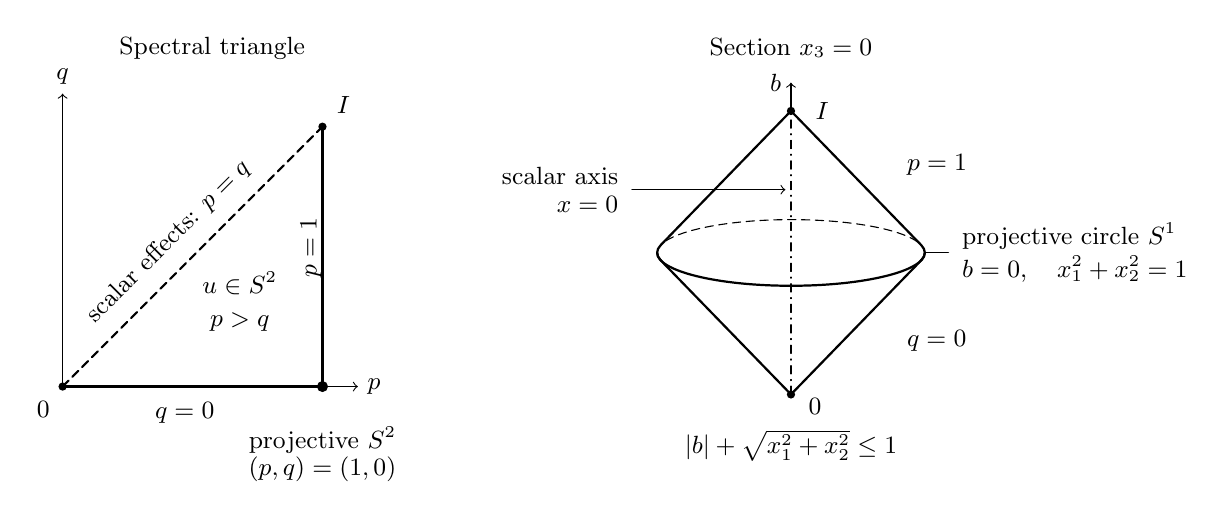
\begin{tikzpicture}[x=1cm,y=1cm,line cap=round,line join=round,
                    font=\small]
  % Left panel: exact ordered spectral triangle.
  \node at (1.9,4.30) {Spectral triangle};
  \draw[->,thin] (0,0) -- (3.75,0) node[right] {$p$};
  \draw[->,thin] (0,0) -- (0,3.72) node[above] {$q$};
  \draw[thick] (0,0) -- (3.3,0) -- (3.3,3.3);
  \draw[thick,densely dashed] (0,0) -- (3.3,3.3);
  \node[rotate=45,anchor=south] at (1.53,1.65)
    {scalar effects: $p=q$};
  \node[anchor=north] at (1.55,-0.08) {$q=0$};
  \node[rotate=90,anchor=south] at (3.41,1.77) {$p=1$};
  \node[align=center] at (2.25,1.08) {$u\in S^2$\\[1pt]$p>q$};
  \fill (0,0) circle (1.5pt);
  \fill (3.3,3.3) circle (1.5pt);
  \fill (3.3,0) circle (2pt);
  \node[anchor=north east] at (-0.04,-0.06) {$0$};
  \node[anchor=south west] at (3.36,3.34) {$I$};
  \node[anchor=north,align=center] at (3.30,-0.39)
    {projective $S^2$\\[-1pt]$(p,q)=(1,0)$};

  % Right panel: a three-dimensional section, shown in linear projection.
  % In local coordinates the map is
  % (x_1,x_2,b) -> (1.70*x_1,0.42*x_2+1.80*b).
  % The cone silhouette meets the projected unit circle at its exact
  % tangency points: sin(alpha)=0.42/1.80=7/30.
  \begin{scope}[shift={(9.25,1.70)}]
    \node at (0,2.60) {Section $x_3=0$};
    \pgfmathsetmacro{\tangentangle}{asin(7/30)}
    \pgfmathsetmacro{\tangentx}{1.70*cos(\tangentangle)}
    \pgfmathsetmacro{\tangenty}{0.42*sin(\tangentangle)}

    \draw[thin,densely dashed] (1.70,0)
      arc[start angle=0,end angle=180,x radius=1.70,y radius=0.42];
    \draw[thick] (-1.70,0)
      arc[start angle=180,end angle=360,x radius=1.70,y radius=0.42];
    \draw[thick] (-\tangentx,\tangenty) -- (0,1.80)
      -- (\tangentx,\tangenty);
    \draw[thick] (-\tangentx,-\tangenty) -- (0,-1.80)
      -- (\tangentx,-\tangenty);
    \draw[thick] (\tangentx,-\tangenty)
      arc[start angle=-\tangentangle,end angle=\tangentangle,
          x radius=1.70,y radius=0.42];
    \draw[thick] (-\tangentx,\tangenty)
      arc[start angle=180-\tangentangle,end angle=180+\tangentangle,
          x radius=1.70,y radius=0.42];

    \draw[thin,dash dot] (0,-1.80) -- (0,1.80);
    \draw[->,thin] (0,1.80) -- (0,2.16) node[left] {$b$};
    \fill (0,1.80) circle (1.5pt);
    \fill (0,-1.80) circle (1.5pt);
    \node[anchor=west] at (0.19,1.80) {$I$};
    \node[anchor=north west] at (0.10,-1.73) {$0$};
    \node[anchor=east,align=right] at (-2.07,0.80)
      {scalar axis\\[-1pt]$x=0$};
    \draw[->,thin] (-2.02,0.80) -- (-0.07,0.80);
    \node[anchor=west] at (1.35,1.12) {$p=1$};
    \node[anchor=west] at (1.35,-1.12) {$q=0$};
    \draw[thin] (1.71,0) -- (2.00,0);
    \node[anchor=west,align=left] at (2.05,0)
      {projective circle $S^1$\\[1pt]$b=0,\quad x_1^2+x_2^2=1$};
    \node[anchor=north] at (0,-2.13)
      {$|b|+\sqrt{x_1^2+x_2^2}\le1$};
  \end{scope}
\end{tikzpicture}
\caption{The four-dimensional effect body $|b|+|x|\le1$.
Each point of the spectral triangle with $p>q$ carries a direction
$u\in S^2$; on the scalar diagonal all directions represent the same
effect. The boundary pieces $q=0$ and $p=1$ meet at the projective stratum
$(p,q)=(1,0)$, which carries the full sphere $S^2$.
The right panel is a projection of the three-dimensional section
$x_3=0$; its equatorial circle is the intersection of that sphere
with the section.}
\label{fig:effectbody76}
\end{figure}

\section{The description entropy of all binary qubit effects}\label{sec:biasedentropy75}
Let
\[
 \mathfrak E=\{E=E^*\in\C^{2\times2}:0\le E\le I\}.
\]
An effect $E$ specifies the ordered measurement with effects $E,I-E$.
Write $\mathcal C_N(\mathfrak E,\delta)$ for its covering number under
$d_N$, allowing arbitrary legal memoryless centres of this interface,
and write $\mathcal C_N^{\mathrm{rat}}(\mathfrak E,\delta)$ when the
centres have rational Cartesian coordinates. Both eigenvalues and the
eigenspaces are charged. The spectral representation
$E=pP_u+q(I-P_u)$, $p\ge q$, represents a scalar effect only once,
independently of $u$.

\begin{theorem}[The full effect body]\label{thm:biasedcover75}
There are absolute constants $c,C,\delta_0>0$ such that, for every integer
$N\ge1$ and $0<\delta\le\delta_0$,
\begin{equation}\label{eq:biasedcover75}
 cN^2\log(N+2)\,\delta^{-4}
 \le \mathcal C_N(\mathfrak E,\delta)
 \le \mathcal C_N^{\mathrm{rat}}(\mathfrak E,\delta)
 \le CN^2\log(N+2)\,\delta^{-4}.
\end{equation}
Consequently the optimum fixed-length reusable payload is
\begin{equation}\label{eq:biasedbits75}
 2\log_2N+\log_2\log(N+2)+4\log_2(1/\delta)+O(1).
\end{equation}
The constants are uniform over the whole closed effect body, including
scalar, deterministic and projective effects. For rational accuracy
input, rational target data admit an exact rational encoder attaining
this order.
\end{theorem}
The logarithm records accumulation near the projective stratum, where
both outcome probabilities can approach their support endpoints.
We prove the upper bound by a finite rational construction and the
lower bound by separated families of projective-corner boxes.

\subsection{A rational spectral and angular code}
For $N\ge1$ and rational $0<\delta\le1/4$, put
\begin{equation}\label{eq:biasedspectralgrid75}
 B=\left\lceil\sqrt{64N/\delta^2}\right\rceil,\qquad
 s_i=\begin{cases}
 \displaystyle\frac{i^2}{B^2+i^2},&0\le i\le B,\\[2mm]
 \displaystyle1-\frac{(2B-i)^2}{B^2+(2B-i)^2},&B<i\le2B.
 \end{cases}
\end{equation}
Thus $0=s_0<s_1<\cdots<s_{2B}=1$. For $0\le j<i\le2B$ define
\begin{equation}\label{eq:biasedangulargrid75}
 K_{ij}^2=
 \frac{N(s_i-s_j)^2}
 {s_i(1-s_i)+s_j(1-s_j)+N^{-1}},\qquad
 A_{ij}=\max\left\{1,
      \left\lceil\sqrt{256K_{ij}^2/\delta^2}\right\rceil\right\}.
\end{equation}
Use the six signed stereographic charts
\begin{equation}\label{eq:biasedsphere75}
 u_a=\epsilon\frac{1-|z|^2}{1+|z|^2},\qquad
 u_b=\frac{2z_b}{1+|z|^2}\quad(b\ne a),\qquad
 a\in\{1,2,3\},\quad \epsilon\in\{-1,1\},
\end{equation}
with $z\in\{-A_{ij},\ldots,A_{ij}\}^2/A_{ij}$ for the spectral
pair $(s_i,s_j)$. Every chart word decodes to
$s_iP_u+s_j(I-P_u)$. A diagonal pair $i=j$ has the single word
$s_iI$. The exact number of words, including redundant chart words,
is
\begin{equation}\label{eq:biasedcapacity75}
 L_{N,\delta}=(2B+1)+
       \sum_{0\le j<i\le2B}6(2A_{ij}+1)^2.
\end{equation}

\begin{theorem}[Exact rational realization]\label{thm:biasedcodec75}
The words in \eqref{eq:biasedcapacity75} form a radius-$\delta/2$
cover of $\mathfrak E$ by legal rational effects, and
\begin{equation}\label{eq:biasedcapacitybound75}
 L_{N,\delta}\le C N^2\log(N+2)\,\delta^{-4}
\end{equation}
for an absolute $C$. If
\[
 E=\tfrac12\bigl((1+b)I+x\cdot\sigma\bigr),\qquad
 b\in\Q,\quad x\in\Q^3,\quad |b|+|x|\le1,
\]
then a covering word is computable by rational arithmetic and integer
comparisons. Its payload is one fixed-length index in the set of
\eqref{eq:biasedcapacity75}.
\end{theorem}
\begin{proof}
Write $f(t)=t^2/(1+t^2)$, $0\le t\le1$. For a probability in
$[0,1/2]$, round its inverse coordinate $t$ to the nearest multiple
of $1/B$; for a probability in $[1/2,1]$, use the reflected chart
$1-f(t)$. Choose the multiple of smaller magnitude at ties. This
defines a nondecreasing quantizer on $[0,1]$, so separately quantizing
$p\ge q$ preserves their order.

The square-root vector associated with $f(t)$ is
$(t,1)/\sqrt{1+t^2}$; its derivative has norm $1/(1+t^2)\le1$.
The reflected chart has the same bound. Hence the Euclidean
square-root distance between each probability and its quantization
is at most $1/(2B)$. If $H$ is this distance, the product-fidelity
inequality gives unhalved distance at most $2\sqrt N H$ between the
corresponding $N$-fold Bernoulli laws. The common two-coin programme
in Lemma~\ref{lem:spectralprojection75} therefore gives a spectral error
at most
\[
                         2\sqrt N/B\le\delta/4.
\]
This argument includes adaptive testers and entangled references.

If the quantized eigenvalues coincide, this completes the encoding.
Otherwise choose a signed chart whose distinguished coordinate has
maximal absolute value in the target direction. Its inverse coordinate
belongs to $[-1,1]^2$. Rounding its two coordinates to the grid of
denominator $A_{ij}$ gives angular error at most $2\sqrt2/A_{ij}$,
since geodesic distance is bounded by the length of the mapped
straight segment and the differential of stereographic projection has
norm at most two. The angular upper bound in Theorem~\ref{thm:biasedangular75}
gives error at most
\[
 \sqrt2 K_{ij}\frac{2\sqrt2}{A_{ij}}
                   \le\delta/4.
\]
The triangle inequality proves the covering assertion. Formula
\eqref{eq:biasedsphere75} preserves the unit sphere exactly, so every
decoded effect is legal and rational.

We verify exact computability even when the input eigenvalues are
irrational. Put $Q=|x|^2\in\Q$. The eigenvalues are
$(1+b\pm\sqrt Q)/2$. Each decision in the spectral rounding compares
one of these numbers with a rational threshold $f((k+1/2)/B)$ or its
reflection. Such a comparison is the sign of a rational number plus
or minus $\sqrt Q$; checking signs before squaring makes it an exact
rational comparison. If $Q=0$, the two quantized eigenvalues coincide.
Otherwise choose the smallest index $a$ maximizing $|x_a|$ and put
$\epsilon=\operatorname{sgn}(x_a)$. The inverse chart is
\[
                    z_b=\frac{x_b}{\sqrt Q+|x_a|}\quad(b\ne a).
\]
Its comparison with any rational rounding threshold again reduces
to the sign of a rational number plus a rational multiple of
$\sqrt Q$. The integers $B,A_{ij}$ are computed by integer squaring
and rational comparison. Thus no irrational normalization is required.
The decoder uses only the displayed rational formulae.

It remains to count the words. Set $m_i=\min(i,2B-i)$ and
$U=B^2/N$. Directly from \eqref{eq:biasedspectralgrid75},
\[
 \frac{m_i^2}{4B^2}\le s_i(1-s_i)\le\frac{m_i^2}{B^2},\qquad
 K_{ij}^2\le
          \frac{4NB^2}{m_i^2+m_j^2+U}.
\]
Each value of $m_i$ occurs at most twice. Since
$(2A_{ij}+1)^2\le C(1+K_{ij}^2/\delta^2)$, we obtain
\begin{equation}\label{eq:biasedlattice75}
 L_{N,\delta}\le CB^2+
 \frac{CNB^2}{\delta^2}
       \sum_{a,b=0}^{B}\frac1{a^2+b^2+U}.
\end{equation}
Here $U\ge1$. The part with $\max(a,b)\le\sqrt U$ is bounded by an
absolute constant. Each successive dyadic square ring contributes
at most another absolute constant. There are at most
$C\log(N+2)$ such rings, because $B/\sqrt U=\sqrt N$. Consequently
\[
              \sum_{a,b=0}^{B}\frac1{a^2+b^2+U}
                       \le C\log(N+2).
\]
Finally $B^2\le CN/\delta^2$, so \eqref{eq:biasedlattice75} proves
\eqref{eq:biasedcapacitybound75}. The support cutoff in the denominator
is retained throughout the count, including the endpoint grid words.
\end{proof}

\subsection{Packing the projective corner}
\begin{proof}[Proof of Theorem~\ref{thm:biasedcover75}]
The upper bound follows from Theorem~\ref{thm:biasedcodec75}. For a
real $\delta$, choose a rational $\delta'$ with
$\delta\le\delta'\le2\delta$ and use its radius-$\delta'/2$ code;
decrease $\delta_0$ to at most $1/8$. For the lower bound first let
$N\ge16$. For every
\[
                     t=8^j/N\le1/16,\qquad j\ge0,
\]
consider the effects with
\begin{equation}\label{eq:biasedcorner75}
 p=1-\alpha,\quad q=\beta,\quad
 t\le\alpha,\beta\le2t,\qquad
 u=u(z),\quad z\in[-1/4,1/4]^2,
\end{equation}
where $u(z)$ is the chart in \eqref{eq:biasedsphere75} with
$a=3,\epsilon=1$. On this square, spherical distance is bounded
above and below by absolute positive multiples of Euclidean distance
in $z$. Throughout \eqref{eq:biasedcorner75}, the eigenvalue gap is
at least $3/4$ and
\[
 p(1-p)\asymp q(1-q)\asymp t,\qquad
 p(1-p)+q(1-q)+N^{-1}\asymp t.
\]
The finite-distance comparison of Theorem~\ref{thm:biasedmetric75}
therefore supplies an absolute $c_1>0$ such that any two points in
this box satisfy
\begin{equation}\label{eq:biasedboxmetric75}
 d_N\ge c_1\min\left\{1,
       \sqrt{N/t}\,
       \bigl| (\alpha,\beta,z)-
              (\alpha',\beta',z')\bigr|_\infty\right\}.
\end{equation}
Choose an absolute sufficiently large $A$ and then an absolute
sufficiently small $\delta_0$. In each of the four coordinates take
a grid of spacing $A\delta\sqrt{t/N}$. Since $Nt\ge1$, this spacing
is at most half the width of either spectral interval when
$\delta\le\delta_0$. The resulting points have pairwise distance
at least $4\delta$ by \eqref{eq:biasedboxmetric75}, and their number
is at least
\[
 c\left(\frac{t}{\delta\sqrt{t/N}}\right)^2
   \left(\frac1{\delta\sqrt{t/N}}\right)^2
                         =cN^2\delta^{-4}.
\]

Points from different boxes are also uniformly separated. Indeed,
if $t'\ge8t$, then $\alpha'\ge t'$ and $\alpha\le2t\le t'/4$.
The spectral modulus of the corresponding upper eigenvalues is
bounded below by an absolute positive multiple of
$\sqrt{Nt'}\ge1$. The spectral noncancellation bound in
Theorem~\ref{thm:biasedmetric75} gives $d_N\ge c_2>0$.
Shrinking $\delta_0$ ensures that this is at least $4\delta$.
There are at least $c\log(N+2)$ permitted boxes. Their union is
therefore a $4\delta$-packing of cardinality
$cN^2\log(N+2)\delta^{-4}$.

For $1\le N<16$, use instead a fixed spectral rectangle
$5/8\le p\le3/4$, $1/4\le q\le3/8$ and the same angular chart.
Theorem~\ref{thm:biasedmetric75} gives a uniform local Euclidean lower
bound, and a grid of spacing $C\delta$ has at least $c\delta^{-4}$
points. The factor $N^2\log(N+2)$ is bounded on this finite range.
This proves the same lower estimate for all $N\ge1$.

A radius-$\delta$ ball about any legal centre contains at most one
point of a $4\delta$-packing, by the triangle inequality. Hence the
packing proves the lower bound with the stated centre convention.
Taking binary logarithms and rounding the index length proves
\eqref{eq:biasedbits75}.
\end{proof}

\subsection{The source of the logarithm}
The spectral and angular weights also give the following integral
form of the same accumulation. Put $v_p=p(1-p)$, $v_q=q(1-q)$ and
$\tau=N^{-1}$. Then
\begin{equation}\label{eq:biasedvolume75}
 \int_{0\le q\le p\le1}
 \frac{N^2(p-q)^2\,dp\,dq}
 {(v_p+v_q+\tau)\sqrt{(v_p+\tau)(v_q+\tau)}}
                         \asymp N^2\log(N+2).
\end{equation}
To verify this, near $p=1,q=0$ put $\alpha=1-p$, $\beta=q$.
After removing the factor $N^2$, the integrand is comparable to
\[
 \frac1{(\alpha+\beta+\tau)
             \sqrt{(\alpha+\tau)(\beta+\tau)}}.
\]
For $s=\alpha+\beta$, integration over $0\le\alpha\le s$ is
bounded above by an absolute constant times $1/(s+\tau)$.
For $s\ge2\tau$, restriction to $s/4\le\alpha\le3s/4$ gives the
matching lower bound. Integration in $s$ proves logarithmic growth.
Near the scalar endpoint $p=q=0$, the factor $(p-q)^2$ is at most
$(p+q)^2$, while $v_p+v_q\asymp p+q$; the remaining integral is
uniformly bounded. Complementation gives the same conclusion near
$p=q=1$. Away from these endpoint neighbourhoods,
$v_p+v_q$ is bounded below and the factors $v_p^{-1/2},v_q^{-1/2}$
are integrable. Bounded $N$ is absorbed into the constants.
Thus the extra logarithm is contributed by the projective corner.
The finite covering construction and packing above also include the
collapsed scalar coordinates, where the spectral representation
ceases to be a chart.

\section{Measurement discrimination, geometry, and learning}
\label{sec:matrixcomparison76}
The present binary interface retains the ordered classical outcome
and an arbitrary external reference, but no postmeasurement quantum
system from the device. This fixes the comparison with the
measurement-discrimination literature. The projective theorem of
Pucha\l a and collaborators \cite[Corollary~1 and Theorem~2]{PPKKO72}
gives an exact multiple-use formula with ancillary access. It is
used in the retained observable-readout theorem. The restricted
ancillary interface in Fiur\'a\v sek--Mi\v cuda \cite{FM75} leads
to a different comparison of adaptive and parallel probes.

Krawiec--Pawela--Pucha\l a \cite[Section~4]{KPP76} construct a pair
of nine-outcome qutrit rank-one POVMs that admit perfect adaptive
discrimination with two calls and no perfect discrimination by
any finite parallel experiment. Datta--Biswas--Saha--Augusiak
\cite[Theorems~3--5]{DBSA76} study entanglement-assisted
single-use discrimination, including perfect constructions and a
qubit entanglement advantage. Their qubit construction has three
outcomes. These are direct antecedents for general POVM
discrimination with a retained reference. They do not supply a
full binary-effect family covering law. Our comparison
\eqref{eq:matrixadaptivity76} permits an adaptive advantage and
controls its size uniformly in $N$ for fixed input dimension.

The differential argument in Lemma~\ref{lem:matrixpath76} belongs
to the established horizontal-gauge and channel-extension method
\cite{FI76,DKG67,DM76,KGAD76}. Finite adaptive discrimination
bounds obtained by integrating a local channel bound appear in
\cite{YF76,SD76}. The binary Sylvester choice here gives the
specific regularized variance $M(I-M)$, which can be integrated
explicitly and matched by compressed nonadaptive tests. The
inverse-Sylvester expressions of Bures geometry
\cite{Dittmann76} and its spectral integration
\cite{SZGeom76} are related methods. Our form acts on the effect
displacement $H$ with variance $V=M(I-M)$; it is not the ordinary
Bures pullback under $M\mapsto V$, whose differential would be
$H-MH-HM$. The operational-ball lemma and the nested endpoint
integral are both required for Theorem~\ref{thm:matrixcover76}.

Mele--Bittel \cite[Lemmas III.7--III.8 and Corollary III.9]{MB67}
give the binary one-use identity and an operator-norm learner.
Zambrano--Ramos-Calderer--Kueng \cite{ZRK76} study one-use outcome
variation under their single-copy probe model. Combining a
one-use $\epsilon$ guarantee with the hybrid bound gives a
future-$N$ guarantee after setting $\epsilon$ of order
$\delta/N$. Theorem~\ref{thm:commonlearn76} instead proves and
matches the order $N\delta^{-2}\log(1/\eta)$ for the future
adaptive loss on all of $\mathfrak E_2$. The learning network of
\cite{BDPS76} stores quantum resources for later measurement
retrieval and has a different output interface.

Multiscale phase estimation and robust phase recovery are
established techniques \cite{HB76,KLY76}. Our proof supplies its
own small-cone argument and conditional confidence allocation;
it does not invoke the numerical unwrapping threshold corrected
by the erratum to \cite{KLY76}. Randomized signs remove the
unknown bias exactly, and empirical amplitudes choose the
entangled block length without a supplied noise parameter.
The learning theorem is a common experiment for all unknown
qubit effects. The pair-dependent tests used in the matrix
metric comparison and the supplied-target exact encoder retain
their separate roles.

All matrix entropy constants are for fixed dimension and small
error. The proof includes every rank and spectral multiplicity
of the binary effect body. Multi-outcome POVMs, residual quantum
outputs, growing-dimension constants, and full submaximal-error
matrix coverings require additional arguments. The inherited
full-error preparation and fixed-readout results retain their
own stated ranges.

\appendix
\section{Rational instruments stable under external references}\label{sec:reference66}
A rounding operation on density matrices need not be affine. In
particular, a nonlinear state repair cannot be tensored with the
identity on an unknown reference system. We therefore round a
\emph{description of the instrument}, once and independently of its
input, rather than round the state on which it acts. The resulting
maps are completely positive and jointly trace preserving. All
constants below are explicit in the input and output dimensions and
the number of outcomes.

\subsection{An integral repair of Choi data}
Write $M_d$ for the complex matrices of order $d$. An instrument from
$M_d$ to $M_n$ with $m$ outcomes is a family of completely positive
maps $\Phi_y$ whose sum is trace preserving. We use the input-first,
\emph{unnormalized} Choi convention
\begin{equation}\label{eq:choiconvention66}
 J_y=\sum_{i,j=1}^d |i\rangle\langle j|\otimes
                     \Phi_y(|i\rangle\langle j|),\qquad
 J_y\ge0,\qquad \sum_{y=1}^m\operatorname{Tr}_{n}J_y=I_d.
\end{equation}
Here $\operatorname{Tr}_{n}$ traces the output factor; in particular
$\sum_y\tr J_y=d$, not one. These are the classical Choi criteria
\cite[Theorems~2.22 and~2.26]{Watrous65}. The channel with the outcome
retained is $\mathcal F(X)=\bigoplus_y\Phi_y(X)$. We write $\|\cdot\|_\diamond$
for the completely bounded trace norm.

\begin{lemma}[Choi trace norm and reference stability]\label{lem:choidiamond66}
For any linear map $\Lambda:M_d\to M_n$ with unnormalized Choi matrix
$J(\Lambda)$,
\[
 d^{-1}\|J(\Lambda)\|_1\le\|\Lambda\|_\diamond
                                      \le\|J(\Lambda)\|_1.
\]
Consequently the diamond distance of two instruments, with the outcome
retained, is at most the sum of the trace norms of their Choi-block
differences.
\end{lemma}
\begin{proof}
Applying $\operatorname{id}_d\otimes\Lambda$ to the normalized
maximally entangled state gives the lower bound. For the upper bound,
let $u,v$ be unit vectors in $\C^r\otimes\C^d$. With
$\Omega=\sum_i e_i\otimes e_i$, write
$u=(A\otimes I_d)\Omega$ and $v=(B\otimes I_d)\Omega$.
The matrices $A,B:\C^d\to\C^r$ have Hilbert--Schmidt norm one and
therefore operator norm at most one. Thus
\[
 (\operatorname{id}_r\otimes\Lambda)(|u\rangle\langle v|)
       =(A\otimes I_n)J(\Lambda)(B^*\otimes I_n)
\]
has trace norm at most $\|J(\Lambda)\|_1$. The trace-norm unit ball
is the convex hull of rank-one partial isometries (including zero as a
convex combination of opposite such matrices). A singular-value
decomposition of an arbitrary input matrix therefore proves the same induced
trace-norm bound, independently of $r$. Taking the supremum over $r$
proves the assertion. For an instrument the Choi matrix is, up to a
fixed permutation of factors, the direct sum of its blocks.
\end{proof}

Let $B$ be a positive integer. The supplied approximations $T_y$ are
Hermitian matrices with entries in $B^{-1}\Z[i]$. Assume that every
independent real diagonal coordinate, and every independent real and
imaginary off-diagonal coordinate, differs from that of $J_y$ by at
most $B^{-1}$. The $T_y$ need not be positive or satisfy the marginal
constraint. Put
\begin{align}
 R&=I_d-\sum_y\operatorname{Tr}_{n}T_y,&
 Q_y&=T_y+\mathbf1_{\{y=1\}}R\otimes|e_1\rangle\langle e_1|,
                                                    \label{eq:choirepair66}\\
 c&=2nd(1+mn),&D&=B+mnc,\qquad
 \widetilde J_y=\frac{BQ_y+cI_{dn}}{D}.\label{eq:choigrid66}
\end{align}
The choice of the first outcome and first output coordinate is merely
a fixed convention. Any fixed outcome and output basis coordinate give
the same legality and uniform error bound. If specified zero outcomes
must remain exactly zero, remove them before applying the theorem and
restore them afterwards; $m$ then counts only the repaired outcomes.

\begin{theorem}[Reference-stable rational instrument rounding]\label{thm:choiround66}
For every $d,n,m,B\ge1$, the matrices in \eqref{eq:choigrid66} are
Choi matrices of an instrument. Their numerators are positive semidefinite matrices with Gaussian-integer entries, their common denominator is $D$, and
\begin{equation}\label{eq:choierror66}
 \|\mathcal F-\widetilde{\mathcal F}\|_\diamond
 \le\sum_y\|J_y-\widetilde J_y\|_1
 \le\frac{3mndc}{B+mnc}\le\frac{K(d,n,m)}B,
 \qquad K(d,n,m)=6mn^2d^2(1+mn).
\end{equation}
The construction uses integer additions, multiplication by specified
integers, and the supplied grid entries. It uses no spectral
factorization, positivity projection, or rational Kraus
factorization. Its complete output description has
\[
 O\bigl(m d^2n^2\log(B+mnc+1)\bigr)
\]
bits, with an absolute implicit constant for the fixed encoding.
\end{theorem}
\begin{proof}
Set $E_y=T_y-J_y$. Counting the real coordinates gives
$\|E_y\|_{\rm op}\le\|E_y\|_F\le2nd/B$.
For a Hermitian $E$, the inequalities
$-\|E\|_{\rm op}I\le E\le\|E\|_{\rm op}I$ imply
$\|\operatorname{Tr}_{n}E\|_{\rm op}\le n\|E\|_{\rm op}$.
It follows that
\[
 \|R\|_{\rm op}\le2mn^2d/B,\qquad
             \|Q_y-J_y\|_{\rm op}\le c/B.
\]
Since $J_y\ge0$, the numerator $BQ_y+cI_{dn}$ is positive.
All its entries are Gaussian integers. The partial trace constraint is
exact, because
\[
 \sum_y\operatorname{Tr}_{n}(BQ_y+cI_{dn})
                       =(B+mnc)I_d.
\]
The Choi criteria therefore give a completely positive instrument,
including when some of the original outcomes are zero.

Let $F_y=Q_y-J_y$. The identity
\[
 D(\widetilde J_y-J_y)=BF_y+cI_{dn}-mncJ_y
\]
and $\|F_y\|_1\le dn c/B$ give
\[
 D\sum_y\|\widetilde J_y-J_y\|_1
 \le mndc+mndc+mnc\sum_y\tr J_y=3mndc.
\]
Lemma~\ref{lem:choidiamond66} proves the norm assertion. Finally each
diagonal entry of a positive numerator is at most $D$, by the summed
partial trace constraint. Positivity bounds every off-diagonal modulus
by the geometric mean of two diagonal entries, hence also by $D$.
Encoding $m(dn)^2$ entries and the common denominator proves the
bit bound. All intermediate entries have polynomially bounded bit
length in the stated parameters and the supplied data.
\end{proof}

For exact rational input, directed truncation supplies $T_y$ by integer
division. For uncertain real input, the hypothesis is a certified error
bound on the \emph{final grid coordinates}; an uncertified floating
estimate is not a premise of the theorem. Although $B$ may be a power
of two, $D=B+mnc$ generally is not. The output is rational, not in
general dyadic. The construction may replace a zero outcome by a
small nonzero one; its mass is charged in \eqref{eq:choierror66}.
Known zero outcomes can instead be removed before rounding and restored
as zero blocks afterwards, with $m$ counting the remaining outcomes.

\begin{corollary}[A finite-description instrument net]\label{cor:instrumentnet66}
For fixed $d,n,m$ and $0<\delta\le1$, the preceding construction yields
a finite diamond-$\delta$ net of legal instruments. Each member has
an integer description of length
\[
 O\bigl(m d^2n^2\log(2+K(d,n,m)/\delta+mnc)\bigr).
\]
This is a deterministic description net, not a statistically learned net.
A particular member is computable in polynomial bit time from rational
input data and the grid precision; enumeration of the entire net is
not required.
\end{corollary}
\begin{proof}
Every Choi diagonal is at most one by \eqref{eq:choiconvention66}, and
positivity bounds every entry modulus by one. There are finitely many
possible directed grid truncations at $B=\lceil K/\delta\rceil$.
Apply the theorem to those arising from valid instruments. Computation
of one truncation and its repair uses a polynomial number of elementary
integer operations on polynomial-length operands.
\end{proof}
The CP/TP constraints and adding a scalar identity buffer are not new
principles. Projected least-squares process tomography already repairs
Choi estimates and uses identity mixing to finish a TP-preserving
positivity correction \cite[Section~4]{PLS66}. Here the particular
integer formula supplies an explicit denominator and a deterministic
diamond-error budget from coordinate errors. No nearest-projection,
statistical sample-complexity, or rank-optimality claim is made.

\subsection{Adaptive use and stopped observations}
A tester may retain an arbitrary finite-dimensional quantum memory,
start with a state entangled across that memory and the instrument
input, and insert arbitrary channels and finite-outcome measurements between uses.
The command port is classical: its value may be selected from the
public history and measured tester memory. Coherent access to a
superposition of commands is not an interface assumed here. The
\emph{same} tester is used in the two compared experiments.

\begin{theorem}[Adaptive reference-stable precision budget]\label{thm:adaptivediamond66}
Suppose that at use $t$, uniformly over permitted commands and public
histories,
$\|\mathcal F_{t,a}-\widetilde{\mathcal F}_{t,a}\|_\diamond\le\delta_t$.
For every common tester with a classical command port (not coherent
superpositions of commands), every initial state, and every public stopping
rule $\tau\le N$, the final states, with the stopped history and tester
memory retained, satisfy
\begin{equation}\label{eq:testererror66}
 \|\Omega_\tau-\widetilde\Omega_\tau\|_1
                  \le\sum_{t=1}^N\delta_t.
\end{equation}
The bound is independent of the tester-memory dimension. In particular,
rounding each command by Theorem~\ref{thm:choiround66} with
$B\ge N K(d,n,m)2^L$ gives stopped joint-state error at most $2^{-L}$
and transcript total-variation error at most $2^{-L-1}$.
\end{theorem}
\begin{proof}
Replace the instruments one use at a time. Just before the replaced
use, both members of a neighboring hybrid pair have the same joint
state. Decomposing a classical command/history register into blocks,
the diamond bound applies to each positive block and is multiplied by
its trace. These traces sum to one. The error introduced at this use
is therefore at most $\delta_t$, including any quantum reference.
All subsequent operations in the hybrid pair are the same channels;
complete trace-norm contraction bounds their final difference by the
same quantity. Summing the $N$ hybrid differences proves
\eqref{eq:testererror66}. For a stopping rule retain an absorbing halt
flag, use the identity on halted blocks, and finish all experiments at
use $N$. A public history-dependent stopping rule is then part of the
same tester. The same argument applies, without conditioning on a
possibly rare stopping history. Taking traces and dividing by two
gives the total-variation assertion.
\end{proof}
The hybrid principle is classical; see
\cite[Section~3.3, equation~(3.306)]{Watrous65} and the operational
strategy norms of \cite{Gutoski66}. The conclusion here is a uniform
finite-description approximation by \emph{genuine instruments}. It is
not a classical device that accepts an unknown physical entangled
state and prepares its output. A numerical simulation of a specified
joint state must charge the joint matrix dimension. Nor does the
nonlinear state repair in the preceding section become a channel by
this theorem.

\begin{proposition}[Posterior control at a stopping time]\label{prop:posterior66}
Let $A_h=p_h\rho_h$ and $\widehat A_h=q_h\widehat\rho_h$ be the
positive blocks at a common bounded stopping time, with both total
traces one. At zero simulated mass assign any density matrix to
$\widehat\rho_h$. If
$\sum_h\|A_h-\widehat A_h\|_1\le\delta$, then
\begin{equation}\label{eq:posterior66}
 \sum_h p_h\|\rho_h-\widehat\rho_h\|_1\le2\delta,\qquad
 \Pr_p\{\|\rho_h-\widehat\rho_h\|_1>\eta\}
                              \le\min\{1,2\delta/\eta\}.
\end{equation}
The tail estimate holds for every $\eta>0$. For any event of true probability $\alpha>0$, the two pooled
conditional states have distance at most $\min\{2,2\delta/\alpha\}$,
with an arbitrary conditional state when the simulated event has
probability zero.
\end{proposition}
\begin{proof}
Writing $e_h=\|A_h-\widehat A_h\|_1$, trace contraction gives
$|p_h-q_h|\le e_h$. For positive $p_h$,
\[
 p_h\|\rho_h-\widehat\rho_h\|_1
 \le e_h+|p_h-q_h|\le2e_h.
\]
The inequality remains valid if $q_h=0$. Sum and apply Markov's
inequality. Applying the same calculation to the sums over an event
gives the final assertion; two density matrices have distance at most
two. Zero true mass makes no contribution.
\end{proof}
The proposition gives weighted, tail and pooled-event posterior control,
not simultaneous accuracy of every normalized rare history.

\section{Exact validation of rational descriptions}
The rational codes below require an exact positivity test. We record
the arithmetic fact in the form used by both encoders.

\begin{lemma}[Reduced Schur entries and bit length]\label{lem:schurminors67}
Let $A$ be a Hermitian matrix of order $q$ with Gaussian-integer entries,
whose real and imaginary parts have absolute value at most $2^h$.
In exact Schur elimination, let $I$ be the ordered indices of the
positive pivots already eliminated. Every remaining entry is
\begin{equation}\label{eq:borderminor67}
 S_{ij}=\frac{\det A[I\mathbin{\|}i,I\mathbin{\|}j]}{\det A[I,I]},
\end{equation}
where $I\mathbin{\|}i$ appends $i$ in that order, and the empty
principal determinant is one. Reduced numerators and denominators
have $O(q(h+\log(q+1)))$ bits. Hermitian positive semidefiniteness is
therefore decidable by this elimination in polynomial bit time and
space in the explicit input length. No optimized polynomial exponent
is asserted.
\end{lemma}
\begin{proof}
When the leading pivot $t$ is positive, block congruence reduces
\[
 \begin{pmatrix}t&b^*\\ b&C\end{pmatrix}\ge0
 \quad\Longleftrightarrow\quad C-bb^*/t\ge0.
\]
A negative pivot rejects. At a zero diagonal, each $2\times2$ principal
minor forces the corresponding row and column to vanish; otherwise
reject, and if they vanish delete that row and column. Positive pivots
make $A[I,I]$ positive definite. The bordered determinant identity
\[
 \det\begin{pmatrix}A[I,I]&A[I,j]\\A[i,I]&A_{ij}\end{pmatrix}
 =\det A[I,I]\,(A_{ij}-A[i,I]A[I,I]^{-1}A[I,j])
\]
proves \eqref{eq:borderminor67}, including after zero rows are skipped.
The specified ordering prevents a spurious permutation sign.

A minor of order $k\le q$ has determinant modulus at most
$k^{k/2}(\sqrt2\,2^h)^k$, by the product of its row norms.
Its real and imaginary parts are integers with
$O(k(h+\log(k+1)))$ bits. The principal denominator is a positive
integer. Cancelling common factors cannot enlarge these lengths.
Each arithmetic operation on reduced Gaussian-rational entries thus
has polynomial operand size. There are polynomially many operations
and at most $q^2$ stored entries; ordinary multiplication, division and
the Euclidean algorithm give the stated bit bounds. For rational
rather than integral input, first clear a common positive denominator.
Its bit length is at most the sum of the encoded denominator lengths,
so this preliminary step also has polynomial cost.
\end{proof}

\section{Intrinsic description entropy of instruments}\label{sec:description67}
We now determine the high-resolution description exponent, rather than
only an upper bound on the number of stored matrix entries. The objects
being described remain genuine quantum instruments. A binary description
of such an object is not a physical classical implementation of it.

Fix positive integers $d,n,m$, put $q=dn$, and use the input-first,
unnormalized Choi convention of Section~\ref{sec:reference66}. Let
\[
 \mathcal C=\mathcal C_{d,n,m}
 =\{(J_y)_{y=1}^m:J_y\in\operatorname{Herm}(q),\ J_y\ge0,
                       \ \sum_y\operatorname{Tr}_n J_y=I_d\}.
\]
The corresponding outcome-retaining channel is denoted by $\mathcal F_J$.
On tuples of Hermitian matrices write
\[
 |X|_2=\left(\sum_y\|X_y\|_F^2\right)^{1/2},\qquad
 \|X\|_{\diamond}=\|\mathcal F_X\|_{\diamond}.
\]
Here $\mathcal F_X$ is the linear map defined by the Choi blocks, whether
or not they are positive. Distances in this section are unhalved norms.
The instrument diamond norm means exactly the diamond norm of this
flagged direct-sum channel, not the sum of the individual outcome-map
diamond norms. All $m$ labeled outcome slots are part of the body.
A legal $\eta$-description code is a finite set of codewords with one
member of $\mathcal C$ assigned to each codeword, such that every target
is within diamond distance $\eta$ of a decoded member. Each codeword
selects one fixed memoryless instrument, not a target-dependent random
mixture with uncharged mixing probabilities. A rational code
requires the decoded matrices to have rational real and imaginary parts.
Dimensions, the outcome names and the requested tolerance are fixed
public parameters in the code-length statements. Their encodings are
additional data when they vary.

\begin{lemma}[Affine dimension and an interior ball]\label{lem:affine67}
The affine hull of $\mathcal C$ has real dimension
\begin{equation}\label{eq:dimension67}
 s=mq^2-d^2=d^2(mn^2-1).
\end{equation}
Let $V=\{X:\sum_y\operatorname{Tr}_n X_y=0\}$ and
$J^\circ_y=I_q/(mn)$. For $X\in V$,
\begin{equation}\label{eq:normequi67}
 |X|_2\le\sum_y\|X_y\|_1\le d\|X\|_{\diamond},\qquad
 \|X\|_{\diamond}\le\sqrt{mq}\,|X|_2.
\end{equation}
The $\|\cdot\|_{\diamond}$-ball in $V$ of radius
$r_0=(dmn)^{-1}$, translated by $J^\circ$, is contained in $\mathcal C$.
Moreover $\mathcal C-J^\circ$ lies in the diamond ball of radius two.
\end{lemma}
\begin{proof}
The map from $\operatorname{Herm}(q)^m$ to $\operatorname{Herm}(d)$
given by summing output partial traces is surjective: an arbitrary
$H\in\operatorname{Herm}(d)$ is the image of the tuple with first block
$H\otimes|e_1\rangle\langle e_1|$ and other blocks zero. Its kernel has
codimension $d^2$. All blocks of $J^\circ$ are positive definite, so
small perturbations in that kernel remain legal. This proves
\eqref{eq:dimension67} and that $V$ is the translation space of the
full affine hull, not merely of a containing affine space.

The first two inequalities follow from Lemma~\ref{lem:choidiamond66}
and the direct-sum Choi matrix. The last follows from that lemma,
$\|X_y\|_1\le\sqrt q\|X_y\|_F$, and Cauchy--Schwarz over $y$.
If $\|X\|_{\diamond}\le r_0$, every block has operator norm at most
$|X|_2\le1/(mn)$, which proves positivity of $J^\circ+X$.
The affine constraint is unchanged. Finally a channel has diamond norm
one, so the distance between any two outcome-retaining channels is at
most two. This also follows from complete trace-norm contractivity of
channels, as in \cite[Corollary~3.40]{Watrous65}.
\end{proof}
The lower Choi estimate from Section~\ref{sec:reference66} thus has a
specific converse use: it transfers a diamond ball into the positive
Choi body. Neither this step nor the dimension count uses a spectral gap.

\begin{theorem}[Sharp high-resolution description exponent]\label{thm:entropy67}
Suppose $s>0$. Let $\mathcal N_{\diamond}(\eta)$ and
$\mathcal N^{\mathbb Q}_{\diamond}(\eta)$ be the smallest cardinalities
of legal and rational legal $\eta$-description codes for $\mathcal C$.
For $0<\eta\le1$,
\begin{equation}\label{eq:cover67}
 \max\{1,(r_0/\eta)^s\}
 \le\mathcal N_{\diamond}(\eta)
 \le\mathcal N^{\mathbb Q}_{\diamond}(\eta)
 \le(1+8/\eta)^s.
\end{equation}
In particular, for fixed $d,n,m$, both optimal fixed-length binary
code lengths are
\begin{equation}\label{eq:bits67}
 s\log_2(1/\eta)+O_{d,n,m}(1)\qquad(\eta\downarrow0).
\end{equation}
When $s=0$, $m=n=1$, the unique instrument is the trace map and the
code length is zero.
\end{theorem}
\begin{proof}
Equip $V$ with Lebesgue measure and the diamond norm restricted to $V$.
By Lemma~\ref{lem:affine67}, the target set contains a ball of radius
$r_0$. A union of $M$ balls of radius $\eta$ covering this ball has
volume at most $M\eta^s$ times the unit-ball volume. Hence
$M\ge(r_0/\eta)^s$. Centres anywhere in the affine hull give the same
lower bound.

For the upper bound, take a maximal set of points of $\mathcal C$
whose mutual distances are greater than $\eta/2$. Balls of radius
$\eta/4$ about them are disjoint up to null boundaries and lie in the
ball of radius $2+\eta/4$ about $J^\circ$. The number of points is
therefore at most $(1+8/\eta)^s$, and maximality makes them an
$\eta/2$-net. Rational legal instruments are dense, by the explicit
construction in Theorem~\ref{thm:intrinsiccodec67} below. Replace each
centre by a rational legal point within $\eta/2$. This yields a rational
$\eta$-net of the same cardinality. This dependence is not circular:
the construction below is proved directly from the Choi constraints.

A codebook with $M$ words can be indexed by $\lceil\log_2M\rceil$ bits,
and a code of at most $b$ fixed-length bits has at most $2^b$ words.
Taking logarithms in \eqref{eq:cover67} proves \eqref{eq:bits67}.
The singleton case follows directly from the constraint $J_1=I_d$.
\end{proof}
This is an elementary volumetric theorem for the precise legal Choi
body and norm. The volume comparison is not a new general covering
principle. The coefficient $s$ is sharp in the high-resolution limit
with dimensions fixed; the estimate does not assert optimal constants
in a simultaneous dimension--accuracy limit.

\subsection{An intrinsic rational coordinate code}
Fix an outcome $y_*$ and an output basis index $\alpha_*$. The
independent real coordinates of a Hermitian matrix are its real diagonal
entries and the real and imaginary parts of its strictly upper-triangular
entries. Omit all $d^2$ such coordinates belonging to the submatrix
\[
 ((J_{y_*})_{i\alpha_*,j\alpha_*})_{1\le i,j\le d}.
\]
There are exactly $s$ remaining real coordinates, in a fixed order.
Every coordinate of a legal target has absolute value at most one:
positivity and the marginal identity bound each diagonal by one, and
$|J_{uv}|^2\le J_{uu}J_{vv}$ bounds the off-diagonal entries.

For $B\in\N$, truncate the $s$ retained coordinates toward zero on
the grid $B^{-1}\Z$, producing digits $z_1,\ldots,z_s\in[-B,B]\cap\Z$.
Fill the omitted submatrix by the exact marginal identity:
\begin{equation}\label{eq:intrinsicfill67}
 (Q_{y_*})_{i\alpha_*,j\alpha_*}
 =\delta_{ij}-
   \sum_{(y,\alpha)\ne(y_*,\alpha_*)}
                         (Q_y)_{i\alpha,j\alpha}.
\end{equation}
All summands on the right were retained. Lower-triangular entries are
Hermitian copies, not additional digits.

\begin{theorem}[Exact intrinsic codec]\label{thm:intrinsiccodec67}
Let
\begin{equation}\label{eq:codeconstants67}
 c=2nd(1+mn),\qquad D=B+mnc,\qquad K=3mndc.
\end{equation}
The matrices
\begin{equation}\label{eq:intrinsicrepair67}
 \widehat J_y=(BQ_y+cI_q)/D
\end{equation}
are positive semidefinite with Gaussian-integer numerators, satisfy
$\sum_y\operatorname{Tr}_n\widehat J_y=I_d$, and obey
\begin{equation}\label{eq:intrinsicerror67}
 \|\mathcal F_J-\mathcal F_{\widehat J}\|_{\diamond}
 \le\sum_y\|J_y-\widehat J_y\|_1\le K/D\le K/B.
\end{equation}
They can be encoded by one integer in $[0,(2B+1)^s)$, using at most
$\lceil\log_2((2B+1)^s)\rceil$ bits. Thus $B=\lceil K/\eta\rceil$
achieves the leading coefficient $s$ in \eqref{eq:bits67} by a direct
coordinate code, without enumerating a net. For rational input,
encoding, decoding and validity testing have polynomial bit complexity
in the explicit input and output lengths. This is not a workspace
bound for a trajectory simulator.
\end{theorem}
\begin{proof}
Non-omitted independent-coordinate errors are at most $1/B$. An omitted
coordinate is reconstructed from at most $mn-1$ errors, so its error
is at most $(mn-1)/B$. In particular every independent real error is
at most $mn/B$. Counting the Hermitian copies gives the safe estimate
\[
 \|Q_y-J_y\|_{\mathrm{op}}\le\|Q_y-J_y\|_F
 \le 2qmn/B\le c/B.
\]
The affine constraint is exact by \eqref{eq:intrinsicfill67}. Therefore
$BQ_y+cI_q\ge0$ and its summed output partial trace is
$(B+mnc)I_d$. With $E_y=Q_y-J_y$,
\[
 D(\widehat J_y-J_y)=BE_y+cI_q-mncJ_y.
\]
The sum of the trace norms of each of the three terms is bounded by
$mndc$, using $\sum_y\operatorname{tr}J_y=d$ for the last term.
Lemma~\ref{lem:choidiamond66} proves \eqref{eq:intrinsicerror67}.

Set $M=2B+1$. The integer with base-$M$ digits $z_j+B$ determines
all retained coordinates, and \eqref{eq:intrinsicfill67} then determines
the omitted coordinates. A fixed number of digits is used, including
leading zeros. Only integers whose reconstructed, buffered blocks are
positive are valid codewords. They can be recognized by the exact
Schur test in Lemma~\ref{lem:schurminors67}. Every code produced from a
legal target is valid by the preceding proof. If a total decoder is
required, assign each invalid word the canonical rational instrument
$J^\circ$; unused binary strings can be treated in the same way.
The valid codebook already covers all targets. In the singleton case
the construction decodes the trace map from the empty string.

For rational data the coordinate digits are obtained by exact signed
integer division. Matrix filling, buffering and base conversion are
finite integer operations with polynomial operand lengths. Exact PSD
validation has polynomial cost by Lemma~\ref{lem:schurminors67}.
No eigenvector computation, rational Kraus factorization, random draw,
statistical sample or floating-point decision is involved. For an
arbitrary real target, the coordinate construction proves existence
and density; it is not an algorithm for recovering unknown real input
from finitely many unverified measurements.
\end{proof}

\begin{remark}[Known zero outcomes and public headers]\label{rem:zerocode67}
If a specified set of outcomes is known to be zero, remove it before
coding and restore it afterwards. With $m'\ge1$ active outcomes the
intrinsic dimension is $d^2(m'n^2-1)$, and $m'$ replaces $m$ in the
constants. If the active set is not a fixed public parameter, its mask
must also be encoded. The generic construction does not preserve zeros
without this operation. The choice of $(y_*,\alpha_*)$ affects neither
the dimension nor the bounds. Headers for dimensions, $B$, outcomes
and the chosen coordinate convention are not part of a fixed-parameter
codeword; a self-contained file carries and charges them separately.
\end{remark}

\section{Description entropy under repeated adaptive use}\label{sec:adaptiveentropy67}
The number of calls changes the precision needed in a reusable
instrument description. On a strictly positive Choi body the relevant
scale is $N^{-1/2}$, not the $N^{-1}$ scale supplied by a general
one-slot hybrid. We prove a finite, multiparameter coding statement
against arbitrary common adaptive quantum testers.

For two instruments $J,L\in\mathcal C_{d,n,m}$, define
\begin{equation}\label{eq:adaptivemetric67}
 d_N(J,L)=\sup_{\mathsf T}
       \|\Omega_J^{\mathsf T}-\Omega_L^{\mathsf T}\|_1.
\end{equation}
Here $\mathsf T$ is the same causal tester in both experiments, uses the
same memoryless instrument at most $N$ times, and may have arbitrary
finite-dimensional quantum memory, initially entangled references,
intermediate quantum channels and measurements, and classical
feedback. Fresh ancillary systems of arbitrary finite dimension are
allowed: each tester has finite-dimensional registers at every slot,
but no common dimension bound is imposed in the supremum.
Outcomes and final memory are retained. A public stopping
time bounded by $N$ is allowed. A changed input dimension can be handled
by a tester channel between calls. There is no coherent superposition
of command ports, no tester informed of the hidden choice $J$ versus
$L$, and no stopping based on inaccessible simulator state. Taking
suprema of trace distances gives the triangle inequality. In
particular $d_N\le2$. Public stopping is included by an absorbing flag,
as in Theorem~\ref{thm:adaptivediamond66}.

For a fixed $a$ with $0<a<1/(mn)$ let
\[
 \mathcal C_a=\{J\in\mathcal C:J_y\ge aI_{dn}\text{ for every }y\}.
\]
This is a Choi eigenvalue margin, not a spectral gap for an action or a
mixing hypothesis on trajectories. Its affine dimension is the same
$s=d^2(mn^2-1)$ as before.

\begin{lemma}[Two-point classical programme bound]\label{lem:programme67}
Suppose $J_y,L_y\ge\lambda I_{dn}$ for every outcome and
$r=|J-L|_2\le\lambda$, where $\lambda>0$. Then, for every $N\ge1$,
\begin{equation}\label{eq:rootN67}
 d_N(J,L)\le\min\{2,\,2\sqrt N\,r/\lambda\}.
\end{equation}
The same bound covers arbitrary initially entangled references and
bounded public stopping in \eqref{eq:adaptivemetric67}.
\end{lemma}
\begin{proof}
There is nothing to prove for $r=0$. Put $K=(J+L)/2$ and
$U=(J-L)/r$. Since $U\in V$ and each $\|U_y\|_{\mathrm{op}}\le1$,
\[
                      K^+=K+\lambda U,\qquad K^-=K-\lambda U
\]
are legal instruments. With
\[
 p_\pm=\tfrac12\pm\frac r{4\lambda},\qquad
 q_\pm=\tfrac12\mp\frac r{4\lambda},
\]
we have $J=p_+K^++p_-K^-$ and $L=q_+K^++q_-K^-$.
All four probabilities are at least $1/4$. The elementary inequality
$\log x\le x-1$ implies
\[
 D(p\|q)\le\sum_{b\in\{+,-\}}\frac{(p_b-q_b)^2}{q_b}
                                      \le\frac{2r^2}{\lambda^2}.
\]
Choose the programme signs independently in advance for all $N$
slots. Conditional on a sign string, a fixed tester acts on exactly
the same sequence of genuine quantum instruments in the two
experiments. It therefore defines one channel from the classical sign
string to the final quantum--classical state. This remains true with
adaptive feedback: conditioning fixes the instruments, not the
tester's outcomes. If the tester stops early, the unused signs are
ignored. Contractivity and the classical product identity give
\[
 \|\Omega_J^{\mathsf T}-\Omega_L^{\mathsf T}\|_1
 \le2\operatorname{TV}(p^{\otimes N},q^{\otimes N})
 \le\sqrt{2N D(p\|q)}\le2\sqrt N\,r/\lambda.
\]
The middle bound is the usual Pinsker inequality. To recall an elementary
proof, coarse-grain two distributions to the set where the first is
larger. The log-sum inequality reduces relative entropy to binary
relative entropy. Its second derivative in the first argument is
$1/[x(1-x)]\ge4$, so integration about its minimum proves
$D\ge2\operatorname{TV}^2$. Taking the supremum over testers proves
the assertion.
\end{proof}
The classical-programme idea is an established method in quantum
metrology; Demkowicz-Dobrza\'nski, Ko\l ody\'nski and Gu\c{t}\u{a}
\cite[Equations~(4)--(6), Methods]{DKG67} use parameter-dependent
mixtures of fixed channels to bound distinguishability. The lemma
above gives the finite two-point trace-norm estimate needed here,
including common adaptive testers and public stopping. It is not a
claim that the mixture method or the square-root scale is a new
metrological principle. The operations $K^\pm$ remain quantum
operations, not classical physical substitutes for unknown input.

\begin{lemma}[Repeated Choi tests]\label{lem:choitesting67}
For any two instruments $J,L\in\mathcal C$, with $t=|J-L|_2$,
\begin{equation}\label{eq:choitesting67}
 d_N(J,L)\ge2-4\exp\left(-\frac{Nt^2}{8d^2}\right).
\end{equation}
A negative right-hand side is simply a vacuous lower bound.
\end{lemma}
\begin{proof}
At each call supply half of a normalized maximally entangled state and
retain its other half and the outcome. The resulting density matrices
are $A=d^{-1}\bigoplus_yJ_y$ and $B=d^{-1}\bigoplus_yL_y$.
They have trace one. The projector on the positive part of $A-B$
gives a binary measurement whose probability gap is
\[
 g=\tfrac12\|A-B\|_1\ge t/(2d).
\]
The same binary measurement is made on each of the $N$ independent
outputs. With a threshold halfway between the two means, each wrong-side
probability is at most $\exp(-Ng^2/2)$. Indeed for a Bernoulli variable
$Z$, the second derivative of
$\log\mathbb E e^{u(Z-\mathbb EZ)}$ is the variance of a tilted
Bernoulli variable and is at most $1/4$. The value and first derivative
at zero vanish; integration and Chernoff's inequality give
$\Pr\{N^{-1}\sum Z_i-\mathbb EZ\ge v\}\le e^{-2Nv^2}$,
and likewise for the other tail. Set $v=g/2$.
The total variation distance between the two product experiments is
at least $1-2e^{-Ng^2/2}$; the unhalved trace norm of their classical
outputs is twice this. This particular nonadaptive tester is allowed
in \eqref{eq:adaptivemetric67}, and the result follows. The tester may
depend on the pair $J,L$, as is permitted when lower-bounding a metric;
it is the same tester for the two members of that pair.
\end{proof}

\begin{theorem}[Sharp horizon exponent for interior descriptions]\label{thm:adaptiveentropy67}
Fix $d,n,m$ with $s>0$, a margin $0<a<1/(mn)$ and a tolerance
$0<\delta<1$. Let $\mathcal M_N(\delta;a)$ be the minimum number of
legal decoded instruments whose $d_N$-balls of radius $\delta$ cover
$\mathcal C_a$. A decoded instrument need not itself have margin $a$.
Write $\mathcal M_N^{\mathbb Q}$ when rational decoded instruments are
required. Set
\[
 R=\frac1{mn}-a,\qquad
 c_\delta=\sqrt{8d^2\log\frac4{1-\delta}},\qquad
 B_N=\left\lceil\frac Ka\left(2+
                         \frac{4\lceil\sqrt N\rceil}{\delta}\right)\right\rceil,
\]
where $K$ is from \eqref{eq:codeconstants67}. Then
\begin{equation}\label{eq:adaptivecover67}
 \max\{1,(R\sqrt N/c_\delta)^s\}
 \le\mathcal M_N(\delta;a)
 \le\mathcal M_N^{\mathbb Q}(\delta;a)
 \le(2B_N+1)^s.
\end{equation}
Consequently the minimum fixed-length description satisfies
\begin{equation}\label{eq:adaptivebits67}
 \log_2\mathcal M_N^{\mathbb Q}(\delta;a)
       =\frac s2\log_2N+O_{d,n,m,a,\delta}(1),
\end{equation}
and the same formula holds without the rationality restriction.
The upper bound is achieved by the exact intrinsic codec applied once
at grid $B_N$; its decoded instrument is reused at every call.
\end{theorem}
\begin{proof}
The tuple-Frobenius ball in $V$ of radius $R$ about $J^\circ$ is
contained in $\mathcal C_a$. Choose a maximal set of points in that
ball with pairwise distances greater than $c_\delta/\sqrt N$.
Balls of that radius about the selected points cover the original
ball. Euclidean volume comparison therefore gives at least
$(R\sqrt N/c_\delta)^s$ points. By Lemma~\ref{lem:choitesting67}, their
pairwise $d_N$ distances are greater than
\[
 2-4e^{-c_\delta^2/(8d^2)}=1+\delta>2\delta.
\]
One $d_N$-ball of radius $\delta$ cannot cover two of these points,
regardless of the location of its legal centre. This proves the lower
bound.

For the upper bound use Theorem~\ref{thm:intrinsiccodec67}. It gives
\[
 r=|J-\widehat J|_2\le\sum_y\|J_y-\widehat J_y\|_1
 \le K/B_N\le\min\{a/2,\ a\delta/(4\sqrt N)\}.
\]
Every block of $\widehat J$ is consequently at least $(a/2)I$, and
both $J$ and $\widehat J$ satisfy Lemma~\ref{lem:programme67} with
$\lambda=a/2$ and $r\le\lambda$. Its conclusion gives
$d_N(J,\widehat J)\le4\sqrt N\,r/a\le\delta$.
There are at most $(2B_N+1)^s$ possible digit strings. All codewords
arising from targets in $\mathcal C_a$ decode legally. The remaining
codewords may be rejected or assigned $J^\circ$; this does not affect
the cover. Since $B_N=O_{d,n,m,a,\delta}(\sqrt N)$, taking logarithms
in \eqref{eq:adaptivecover67} proves \eqref{eq:adaptivebits67}.
\end{proof}

\begin{remark}[What is charged]\label{rem:adaptivescope67}
The lower bound concerns the number of possible reusable mathematical
instrument descriptions, not the mutable memory of a simulator that
receives and stores the entire instrument as input. It applies to all
full-dimensional strictly positive instrument families above, without
an expanding unitary subsystem. It therefore complements, rather than
replaces, the hypothesis-sensitive streaming-space lower bounds.
For variable $a,\delta,d,n,m$, the displayed finite inequalities remain
valid; \eqref{eq:adaptivebits67} holds with those parameters fixed.
The estimates of this section alone assert neither an optimal uniform
dimension constant nor a complete joint $N$--$\delta$ asymptotic.
The latter is supplied, for fixed dimensions and margin, by
Theorem~\ref{thm:jointcode68}. The rational implementation takes
rational $a,\delta$ and an asserted margin, which it can verify exactly.
No samples of an unknown channel are supplied or required.
\end{remark}

\begin{proposition}[The boundary is quantitatively different]\label{prop:boundaryphase67}
There is no constant $C$ such that
$d_N(J,L)\le C\sqrt N\,|J-L|_2$ holds for every pair of qubit channels
and every $N$. In particular the strict margin in
Theorem~\ref{thm:adaptiveentropy67} cannot be removed from its proof by
setting $a=0$.
\end{proposition}
\begin{proof}
Let $U_\theta=\operatorname{diag}(1,e^{i\theta})$ and compare its
unitary channel to the identity channel. For their unnormalized Choi
matrices,
\[
 |J(U_\theta)-J(I)|_2
       =2\sqrt2\,|\sin(\theta/2)|\le\sqrt2\,|\theta|.
\]
At $\theta=\pi/N$, sequentially applying the unknown channel $N$
times to $|+\rangle$ gives respectively $|-\rangle$ and $|+\rangle$.
The final trace distance is two. The proposed upper bound would tend
to zero. The general additive diamond hybrid remains valid at this
boundary; the proposition asserts no global covering exponent for
boundary or rank-constrained instrument classes.
\end{proof}

\subsection{Description, learning and physical simulation}
A reusable rational description is different from a protocol that
replaces quantum communication by classical messages.
Naik, Zartab, Gisin and Banik \cite[Theorems~2 and~5]{NZGB67} show a
finite-classical-message obstruction for the perfect qubit channel in
a reference-sensitive joint-measurement model, and finite-resource
possibility for noisy depolarizing channels. Their receiver retains a
quantum system; the task is physical simulation. Here the decoded
objects and the vertices in Lemma~\ref{lem:programme67} are genuine
quantum instruments. Our numerical algorithms instead start from
specified matrices. Neither construction supplies a classical physical
device accepting unknown entangled input.

Unknown-channel learning charges channel queries used to infer a
classical description. Mele and Bittel \cite[Theorem~I.1]{MB67}
prove dimension-optimal query complexity at fixed diamond accuracy;
Oufkir and Girardi \cite{OG67} give further accuracy-dependent query
lower bounds. The input here is already specified, and the lower bound
in \eqref{eq:adaptivecover67} counts descriptions, not the queries
needed to select one from unknown data. The elementary packing and
testing ingredients are shared methods, not a priority claim that
those learning theorems are consequences of this code.

\section{Joint horizon and accuracy in description length}\label{sec:jointdescription68}
The exponential test in Lemma~\ref{lem:choitesting67} resolves pairs at
fixed error, but its lower bound is vacuous when the two experiments are
very close. A bounded statistic gives the local estimate needed to retain
the accuracy parameter. Throughout this section $N\ge1$ and the adaptive
distance $d_N$ is the unhalved final-state trace distance maximized over
one common tester, as in \eqref{eq:adaptivemetric67}. The unknown device
is the same memoryless instrument at every call; commands are classical,
and stopping is public and bounded by $N$.

\begin{lemma}[A local binary test]\label{lem:binarylocal68}
For $0\le p,q\le1$,
\begin{equation}\label{eq:binarylocal68}
 \TV\bigl(\operatorname{Bern}(p)^{\otimes N},
          \operatorname{Bern}(q)^{\otimes N}\bigr)
 \ge \frac3{32}\min\{\sqrt N\,|p-q|,1\}.
\end{equation}
The estimate is uniform up to the endpoints of the probability interval.
\end{lemma}
\begin{proof}
Assume $p<q$ and first suppose $q-p\le N^{-1/2}$. Put
$b=N(p+q)/2$ and let $f:\R\to[0,1]$ be the nondecreasing function
which is affine with slope $(8\sqrt N)^{-1}$ on
$[b-4\sqrt N,b+4\sqrt N]$, zero to its left, and one to its right.
For $S\sim\operatorname{Bin}(N,t)$, differentiating the finite binomial
polynomial gives the exact identity
\[
 \frac d{dt}\E_t f(S)
 =N\E_t\{f(T+1)-f(T)\},\qquad T\sim\operatorname{Bin}(N-1,t).
\]
It holds on $(0,1)$ and extends continuously to both endpoints. For
$t\in[p,q]$, the distance from $\E_tT$ to $b$ is at most
$\sqrt N/2+1$. Also $\operatorname{Var}_tT\le(N-1)/4$. Chebyshev's
inequality gives
\[
 \Pr_t\{|T-\E_tT|\le\sqrt N\}\ge3/4.
\]
On this event, both $T$ and $T+1$ belong to the affine interval:
their distance to $b$ is at most $3\sqrt N/2+2\le4\sqrt N$.
Since $f$ is nondecreasing everywhere,
\[
 \frac d{dt}\E_t f(S)\ge\frac3{32}\sqrt N.
\]
Integration from $p$ to $q$, and the characterization of total
variation by $[0,1]$-valued statistics, prove the assertion in this
case. The statistic depends only on the count, which is a function
of the full binary string.

If $q-p>N^{-1/2}$, apply the same construction to
$p$ and $q_0=p+N^{-1/2}<q$. Couple Bernoulli samples by common
uniform random variables. Monotonicity of $f$ then gives
$\E_qf(S)\ge\E_{q_0}f(S)$, and the preceding lower bound is $3/32$.
The cases $p=q$ and $q<p$ follow by equality and symmetry.
\end{proof}
The proof uses only binomial differentiation and a bounded statistic;
it requires neither a normal approximation nor a lower variance bound.
In particular its constant does not deteriorate for a rare outcome.

\begin{corollary}[Local repeated Choi separation]\label{cor:localchoi68}
For the instrument body $\mathcal C_{d,n,m}$, let $t=|J-L|_2$.
Then
\begin{equation}\label{eq:localchoi68}
 d_N(J,L)\ge\frac3{16}
                  \min\left\{\frac{\sqrt N}{2d}t,1\right\}.
\end{equation}
\end{corollary}
\begin{proof}
Use the same normalized Choi inputs as in
Lemma~\ref{lem:choitesting67}. The positive spectral projection of
$d^{-1}\bigoplus_y(J_y-L_y)$ defines a binary test with probability
gap at least $t/(2d)$. Repeating this test independently and applying
Lemma~\ref{lem:binarylocal68} gives \eqref{eq:localchoi68}; classical
trace distance is twice total variation. This is one admissible
nonadaptive tester. For each pair it is the same tester in both
experiments, and it is allowed in the supremum defining $d_N$.
\end{proof}

\begin{theorem}[The joint interior coding law]\label{thm:jointcode68}
Fix $d,n,m$ with $s=d^2(mn^2-1)>0$ and $0<a<1/(mn)$.
For all $N\ge1$ and $0<\delta\le1/32$,
\begin{equation}\label{eq:jointcode68}
 \max\left\{1,\left(\frac{R\sqrt N}{32d\delta}\right)^s\right\}
 \le\mathcal M_N(\delta;a)
 \le\mathcal M_N^{\Q}(\delta;a)\le(2B_N+1)^s,
\end{equation}
where $R=1/(mn)-a$ and $B_N$ is the explicit grid in
Theorem~\ref{thm:adaptiveentropy67}. Consequently the optimal legal
fixed-length description, with or without rational decoded matrices,
has length
\begin{equation}\label{eq:jointbits68}
 \frac s2\log_2N+s\log_2(1/\delta)+O_{d,n,m,a}(1),
\end{equation}
uniformly on this whole range of $N$ and $\delta$. The decoded
instrument is reused unchanged, and no spectral-gap hypothesis occurs.
\end{theorem}
\begin{proof}
The tuple-Frobenius ball of radius $R$ about $J^\circ$ in $V$ is
contained in $\mathcal C_a$. Take a maximal set in this ball whose
pairwise Euclidean distances are greater than
$h=32d\delta/\sqrt N$. Maximality and $s$-dimensional volume give at
least $(R/h)^s$ points. Corollary~\ref{cor:localchoi68} separates
each pair by more than $2\delta$ in $d_N$: before the minimum saturates
its value is greater than $3\delta$, and after saturation it is
$3/16>2\delta$. Thus no legal centre of a $d_N$-ball of radius
$\delta$ can cover two packing points, even if that centre has no
positive eigenvalue margin. This proves the lower bound.

The intrinsic rational codec and its classical-programme estimate in
Theorem~\ref{thm:adaptiveentropy67} give the upper bound with the
same $B_N$. Since $N\ge1$ and $\delta\le1/32$, there is a constant
$C=C(d,n,m,a)$ such that $2B_N+1\le C\sqrt N/\delta$. The lower
bound and this inequality give \eqref{eq:jointbits68}, including
rounding a logarithm up to a fixed-length binary code. When the
volumetric lower expression is less than one, its logarithm is negative;
the nonnegative code length still gives the same uniform additive
estimate. Neither bound charges the queries of a learning procedure.
\end{proof}
The earlier fixed-error theorem is retained. The new assertion is the
uniform additive remainder in \eqref{eq:jointbits68}, which is
independent of both the horizon and the accuracy. It does not assert
sharp dimension-dependent constants, nor is it a lower bound for the
mutable workspace of the variable-description trajectory algorithm.

\section{Boundary-uniform coding of preparation instruments}\label{sec:boundarycode68}
Strict positivity is essential to the two-point programme argument, as
Proposition~\ref{prop:boundaryphase67} shows. Nevertheless it is not
necessary for a complete coding law in an irreversible family. We
consider all outcome-retaining instruments that erase their input and
prepare a specified quantum--classical state. This family contains zero
outcomes and arbitrary rank-deficient output blocks.

For $m,n\ge1$ put
\[
 \mathcal S_{m,n}=\{(\sigma_y)_{y=1}^m:\sigma_y\in\operatorname{Herm}(n),
                  \ \sigma_y\ge0,\ \sum_y\tr\sigma_y=1\}.
\]
Write $\boldsymbol\sigma=\bigoplus_y\sigma_y$. For any input
dimension $d\ge1$, the associated instrument is
\begin{equation}\label{eq:replacer68}
 \mathcal R_{\sigma,y}(X)=\tr(X)\sigma_y,\qquad
 J_y(\mathcal R_\sigma)=I_d\otimes\sigma_y.
\end{equation}
The output label $y$ is retained. Its conditional quantum state is
$\sigma_y/\tr\sigma_y$ when that trace is positive. This is a
specified mathematical quantum instrument; a description of it is not
a numerical algorithm acting on an unknown physical input.

\begin{lemma}[Reduction to a product-state experiment]\label{lem:productreplacer68}
For arbitrary $\sigma,\tau\in\mathcal S_{m,n}$,
\begin{equation}\label{eq:productreplacer68}
 d_N(\mathcal R_\sigma,\mathcal R_\tau)
   =\|\boldsymbol\sigma^{\otimes N}
                -\boldsymbol\tau^{\otimes N}\|_1.
\end{equation}
Here the tester may have arbitrary quantum memory, initial reference
entanglement, feedback and a public stopping time at most $N$.
\end{lemma}
\begin{proof}
Supply $N$ independent program states $\boldsymbol\sigma$ to one
fixed processor. At the next device call the processor discards the
incoming device system and returns the next program state, including
its classical outcome. Between calls it performs the prescribed tester
operations. This reproduces the experiment exactly, even when the
incoming system is entangled with the tester memory: the incoming
system is traced out in \eqref{eq:replacer68}. Unused program states
are ignored after a public stop. The processor is the same channel
for $\sigma$ and $\tau$, so trace-norm contraction gives the upper
bound. Conversely, a tester can make exactly $N$ calls and retain
every outcome and quantum output. Its final state is the displayed
product, which proves equality. The processor is a quantum channel,
not a claimed finite-classical-message physical simulator.
\end{proof}

\subsection{Triangular factors and a rational code}
Every $\sigma\in\mathcal S_{m,n}$ has triangular factors
$L_y$ with $\sigma_y=L_yL_y^*$ and nonnegative real diagonal entries.
The usual no-pivot Cholesky procedure also covers singular matrices:
a zero diagonal pivot forces the entire residual row and column to
vanish and contributes a zero factor column. A block of rank $r$
therefore has exactly $r$ positive pivots. All factors together satisfy
$\sum_y\|L_y\|_F^2=1$.

Fix public bounds $0\le r_y\le n$, not all zero, and write
\begin{equation}\label{eq:rankdimension68}
 D=\sum_{y=1}^m r_y(2n-r_y),\qquad v=D-1,
 \qquad
 \mathcal S_{\boldsymbol r}
   =\{\sigma\in\mathcal S_{m,n}:\operatorname{rank}\sigma_y\le r_y\}.
\end{equation}
If the positive pivot positions of $L_y$ are $T_y\subseteq\{1,\ldots,n\}$,
record only the real diagonal and the real and imaginary coordinates
strictly below each such pivot. Their total number is
\[
 h=\sum_y\sum_{j\in T_y}\{1+2(n-j)\}\le D.
\]
The resulting real coordinate vector $x\in\R^h$ has norm one.
The inequality follows by placing each block's pivots as early as
possible. It holds also when the actual ranks are smaller than the
public bounds.

Choose a coordinate $j$ of maximal absolute value, put $a=|x_j|$,
and set $w=x/a$. For an integer $B\ge1$, take
\begin{equation}\label{eq:factorgrid68}
 z_j=B\operatorname{sgn}(x_j),\qquad
 z_i=\operatorname{sgn}(x_i)\lfloor B|w_i|\rfloor\quad(i\ne j).
\end{equation}
Insert these integers in the recorded factor positions to obtain
Gaussian-integer triangular matrices $Z_y$; all unrecorded columns
are zero. Define
\begin{equation}\label{eq:factoroutput68}
 T=\sum_y\|Z_y\|_F^2,\qquad
 \widehat\sigma_y=Z_yZ_y^*/T.
\end{equation}
Since $|z_j|=B$, the denominator satisfies $B^2\le T\le hB^2$.

\begin{theorem}[A boundary-uniform rational factor code]\label{thm:factorcode68}
The output \eqref{eq:factoroutput68} lies in
$\mathcal S_{\boldsymbol r}$, preserves every zero target outcome,
and does not increase the rank of any individual block. For all
$N\ge1$,
\begin{equation}\label{eq:factorerror68}
 d_N(\mathcal R_\sigma,\mathcal R_{\widehat\sigma})
 \le\min\left\{2,\frac{4\sqrt{N(h-1)}}B\right\}
 \le\min\left\{2,\frac{4\sqrt{Nv}}B\right\}.
\end{equation}
At fixed $m,n,\boldsymbol r,B$ a fixed-length code needs at most
\begin{equation}\label{eq:factorbits68}
 mn+\left\lceil\log_2\bigl(2D(2B+1)^v\bigr)\right\rceil
\end{equation}
bits. For rational target blocks, its encoder and decoder use exact
rational and integer arithmetic, including integer square roots; no
algebraic-number oracle, positive eigenvalue margin, or Kraus
factorization is required.
\end{theorem}
\begin{proof}
The product $Z_yZ_y^*$ is positive semidefinite, and normalization
makes the sum of its traces exactly one. Its number of possibly nonzero
columns is no larger than that of $L_y$, so its rank does not exceed
the target rank. When an outcome is zero it has no recorded columns
and remains exactly zero.

Put $z'=z/B$. Its $j$th coordinate agrees with that of $w$; every
other coordinate differs by less than $1/B$. Both $\|w\|$ and
$\|z'\|$ are at least one. The elementary normalization estimate gives
\begin{equation}\label{eq:factornormalize68}
 \left\|x-\frac z{\|z\|}\right\|
 \le\frac{2\|w-z'\|}{\|w\|}
 \le\frac{2\sqrt{h-1}}B.
\end{equation}
Use the normalized vectors
\[
 |L\rangle=\sum_{y,i,j}(L_y)_{ij}|y,i\rangle|y,j\rangle,
 \qquad
 |\widehat L\rangle=T^{-1/2}\sum_{y,i,j}(Z_y)_{ij}|y,i\rangle|y,j\rangle.
\]
Their reduced states on the first factor are
$\boldsymbol\sigma$ and $\widehat{\boldsymbol\sigma}$. Their vector
distance is the left side of \eqref{eq:factornormalize68}. For any
unit vectors $u,v$, diagonalization on their two-dimensional span gives
\[
 \||u\rangle\langle u|^{\otimes N}
       -|v\rangle\langle v|^{\otimes N}\|_1
   =2\sqrt{1-|\langle u,v\rangle|^{2N}}
   \le2\sqrt N\,\|u-v\|.
\]
Indeed $1-t^N\le N(1-t)$ on $[0,1]$ and
$1-|\langle u,v\rangle|^2\le2(1-\Re\langle u,v\rangle)$.
Taking partial traces and using Lemma~\ref{lem:productreplacer68}
proves \eqref{eq:factorerror68}. These are standard purification and
product-fidelity estimates; see \cite[Section~3.2]{Watrous65}. Their
short proof specifies the normalization used here.

The pivot sets use $mn$ bits. Given them, there are at most $2h$
anchor/sign choices and $(2B+1)^{h-1}$ remaining digit strings.
Pad their index to the maximum length in \eqref{eq:factorbits68}.
An invalid header may be rejected, or sent by a total mathematical
decoder to a fixed legal state. Valid factor words always decode
positively, even if they did not arise from this encoder.

For rational input, maintain the exact rational Schur residual $A$.
At a positive pivot $u=A_{jj}$, the factor diagonal is $\sqrt u$
and a lower entry is $A_{ij}/\sqrt u$. Thus the square of each of
its real coordinates is rational, respectively $u$, or
$(\Re A_{ij})^2/u$, or $(\Im A_{ij})^2/u$; its sign is known.
Updating the residual uses rational arithmetic only. Choose the
largest squared coordinate $b_j>0$ by exact comparisons. If another
coordinate has squared value $b_i$, then
\[
 \lfloor B|w_i|\rfloor
   =\operatorname{isqrt}\!\left(\left\lfloor B^2b_i/b_j\right\rfloor\right).
\]
Consequently no square root of a rational number must be represented.
The ratios-of-minors bounds in Lemma~\ref{lem:schurminors67} give
polynomial operand lengths during this preprocessing. Integer square
root, products and mixed-radix coding have polynomial bit complexity
in the explicit input and output lengths. Encoding workspace and the
expanded decoded matrix are not identified with the compressed payload.
\end{proof}

\subsection{Sharp description laws on the boundary}
Let $\mathcal P_N(\delta;\boldsymbol r)$ be the minimum number of
legal preparation instruments whose $d_N$-balls of radius $\delta$
cover $\mathcal S_{\boldsymbol r}$; the decoded centre may have any
output rank. Add a superscript $\Q$ when rational centres are required.
For an upper construction our centres will obey the same rank bounds.

\begin{theorem}[Rank-stratified joint coding law]\label{thm:rankentropy68}
Fix $m,n,\boldsymbol r$ as in \eqref{eq:rankdimension68}. If $v>0$,
there exist constants $c,C>0$, depending only on these fixed data,
such that, for every $N\ge1$ and $0<\delta\le1/32$,
\begin{equation}\label{eq:rankcover68}
 \max\{1,(c\sqrt N/\delta)^v\}
 \le\mathcal P_N(\delta;\boldsymbol r)
 \le\mathcal P_N^{\Q}(\delta;\boldsymbol r)
 \le C(\sqrt N/\delta)^v.
\end{equation}
The optimal legal and rational fixed-length descriptions therefore have
length
\begin{equation}\label{eq:rankbits68}
 \frac v2\log_2N+v\log_2(1/\delta)+O_{m,n,\boldsymbol r}(1)
\end{equation}
uniformly in $N$ and $\delta$. The statement has no spectral-gap or
positive-eigenvalue-margin hypothesis. It includes every rank-deficient
boundary allowed by the public bounds. If $v=0$, the family is a
singleton and its optimal description length is zero.
\end{theorem}
\begin{proof}
For the upper bound take $B=\lceil4\sqrt{Nv}/\delta\rceil$ in
Theorem~\ref{thm:factorcode68}; for rational implementation it suffices
to replace $\sqrt{Nv}$ by its integer ceiling. Its error is at most
$\delta$, and its codebook cardinality is at most
$2^{mn}2D(2B+1)^v$. This has the asserted upper order uniformly on
the stated parameter range.

For completeness we construct a full-dimensional local patch for the
lower bound. For every block with $r_y>0$, take an $n$ by $r_y$
lower-trapezoidal factor: entries above the first $r_y$ diagonal
positions vanish, and these diagonal entries are positive real
numbers. These factors have $D$ independent real coordinates. Impose
$\sum_y\|L_y\|_F^2=1$ and work near the point with all these diagonal
entries equal to $(\sum_y r_y)^{-1/2}$ and all other entries zero.
An open patch of this unit sphere is a smooth $v$-dimensional manifold.
The map
\[
                         (L_y)_y\longmapsto(L_yL_y^*)_y
\]
is one-to-one there and has a smooth inverse on its image. To see the
inverse explicitly, the leading $r_y$ by $r_y$ principal block is
positive definite and determines its unique positive-diagonal Cholesky
factor $A_y$. The bottom-left block is $B_yA_y^*$, so it determines
$B_y$ by multiplication by $(A_y^*)^{-1}$. These operations are smooth
near the chosen point. When $r_y=0$, the entire block is identically
zero and contributes no coordinate.

Choose a closed coordinate ball of sufficiently small positive radius
inside this patch. The chart and its inverse have bounded derivatives
on a slightly larger neighborhood; hence distances between parameters
in the ball are bounded above and below by constant multiples of the
tuple-Frobenius distance between their states. More explicitly one
may bound the derivative of the inverse on a convex neighborhood of
the chosen positive principal blocks, where the same Cholesky formulas
extend smoothly. A maximal Euclidean packing of this parameter ball
at scale $A\delta/\sqrt N$ therefore has at least
$(c\sqrt N/\delta)^v$ points whose state distances exceed
$32\delta/\sqrt N$, after increasing the fixed $A$.

The binary argument of Corollary~\ref{cor:localchoi68}, applied
directly to the trace-one block states (input dimension one), separates
each pair by more than $2\delta$ after $N$ copies. By
Lemma~\ref{lem:productreplacer68} the same separation holds in $d_N$.
One radius-$\delta$ ball, regardless of the rank of its legal centre,
cannot contain two packing points. This proves the lower bound and
then \eqref{eq:rankbits68}. Finally $D=1$ requires $n=1$ and exactly
one bound $r_y=1$; all other bounds vanish. The sole permitted state
has unit mass on that outcome, as asserted.
\end{proof}

\begin{corollary}[All ranks, with an explicit lower constant]\label{cor:fullboundary68}
For the full family $\mathcal S_{m,n}$ put $v=mn^2-1>0$. Then
\begin{equation}\label{eq:fullboundary68}
 \max\left\{1,\left(\frac{\sqrt N}{64mn\delta}\right)^v\right\}
 \le\mathcal P_N(\delta)\le\mathcal P_N^{\Q}(\delta)
 \le 2^{mn}2mn^2(2B+1)^v,
 \qquad B=\left\lceil\frac{4\sqrt{Nv}}\delta\right\rceil.
\end{equation}
In particular a general $n$-dimensional prepared state has coefficient
$n^2-1$, while the class of pure prepared states has coefficient
$2n-2$ in \eqref{eq:rankbits68}. A classical $m$-outcome law has
coefficient $m-1$, including probabilities equal to zero.
\end{corollary}
\begin{proof}
The upper bound is Theorem~\ref{thm:factorcode68} with every $r_y=n$.
For the lower bound, the affine space of block states has dimension
$mn^2-1$. Its tuple-Frobenius ball of radius $1/(2mn)$ about the
blocks $I_n/(mn)$ lies in $\mathcal S_{m,n}$. Repeat the packing proof
of Theorem~\ref{thm:jointcode68} with input dimension one. For pure
states take $m=1,r_1=1$ in Theorem~\ref{thm:rankentropy68}; for
classical laws take $n=1$.
\end{proof}

\begin{remark}[Operational and priority distinctions]\label{rem:boundaryscope68}
Input erasure is decisive in \eqref{eq:productreplacer68}. No analogous
product-state reduction has been proved here for an arbitrary disturbing
instrument; coherent accumulation for unitary channels remains governed
by Proposition~\ref{prop:boundaryphase67}. The present theorems classify
reusable description lengths in the stated preparation families, not
general simulator workspace. Constants remain dimension dependent.

Quantum population compression starts with physical copies of an
unknown state and compresses their quantum information. Yang, Bai,
Chiribella and Hayashi \cite{YBCH68} obtain a half-parameter-count
logarithmic memory law in that different task and show a limitation
on purely classical compression of noncommuting families. Here the
encoder is given a classical matrix description, and each codeword
specifies a state or preparation instrument. It need not infer that
word from unknown copies. The common half-dimension scale, purification
inequalities and finite-dimensional covering methods are classical
antecedents, not claimed inventions. The contribution established here
is a uniform two-parameter legal-description law with a rational,
zero-outcome-preserving, rank-nonincreasing encoder and matching lower
bounds throughout the declared boundary families.
\end{remark}

\section{Retraction of covering centres for preparation targets}\label{sec:centres70}
The centres in a covering problem need not belong to the family being
covered. For preparation targets this distinction can be removed exactly,
without a small-error or rank assumption. Throughout this section a centre
is one memoryless instrument, reused at every call; it is not a device with
an additional persistent environment.

\begin{theorem}[Preparation-centre retraction]\label{thm:retraction70}
Let $\mathcal C=(\mathcal C_y)_{y=1}^m$ be any instrument from $M_d$ to
$M_n$, and set
\begin{equation}\label{eq:retraction70}
 \tau_y=\mathcal C_y(I_d/d)=d^{-1}\operatorname{Tr}_{\rm in}J_y(\mathcal C),
 \qquad \mathfrak R\mathcal C=\mathcal R_\tau.
\end{equation}
Then $\mathfrak R$ maps legal instruments to preparation instruments,
fixes every preparation instrument, and preserves rational Choi data.
For every $N\ge1$ and every $\sigma\in\mathcal S_{m,n}$,
\begin{equation}\label{eq:centredominance70}
 d_N(\mathcal R_\sigma,\mathfrak R\mathcal C)
                  \le d_N(\mathcal R_\sigma,\mathcal C).
\end{equation}
Here $d_N$ is the unhalved trace distance optimized over the common
adaptive testers of Lemma~\ref{lem:productreplacer68}. Consequently, for
any subset of preparation targets and any radius $\delta>0$, the minimum
covering cardinality is unchanged when arbitrary legal memoryless centres
are restricted to preparation centres. The assertion also holds when
centres are required to have rational Choi entries.
\end{theorem}
\begin{proof}
Complete positivity gives $\tau_y\ge0$, and trace preservation gives
$\sum_y\tr\tau_y=1$. The formula is rational and is the identity on the
preparation family, so $\mathfrak R^2=\mathfrak R$. Feed the state $I_d/d$
into each of $N$ calls to $\mathcal C$, use a fresh input at the next call,
and retain all outputs and outcome labels. The resulting state is
$\boldsymbol\tau^{\otimes N}$, since the centre is memoryless. The same
tester applied to $\mathcal R_\sigma$ returns
$\boldsymbol\sigma^{\otimes N}$. Therefore
\[
 \|\boldsymbol\sigma^{\otimes N}-\boldsymbol\tau^{\otimes N}\|_1
                        \le d_N(\mathcal R_\sigma,\mathcal C).
\]
Lemma~\ref{lem:productreplacer68} identifies the left side with the left
side of \eqref{eq:centredominance70}. Retracting every centre in any cover
preserves coverage and cannot increase cardinality. The reverse inequality
follows because preparation centres are among the legal centres. The same
argument preserves rationality.
\end{proof}

The retraction does not preserve a target rank bound: for example the
identity channel retracts to the maximally mixed preparation. Thus the
centre restriction in Theorem~\ref{thm:retraction70} is to the full
preparation family, not necessarily to the target rank stratum. The
rank-constrained rational upper centres of
Theorem~\ref{thm:factorcode68} remain a separate, stronger construction.
The theorem concerns the geometry of mathematical descriptions. Its
maximally mixed test is a quantum experiment, not a finite-classical-message
simulation of unknown inputs.

The reduction mechanism for input-erasing channels has a direct antecedent
in Cooney--Mosonyi--Wilde \cite{CMW70}. Their discussion of two replacer
channels reduces channel divergences to state divergences; their principal
results concern asymptotic discrimination and strong-converse exponents
for a channel versus a replacer. Lemma~\ref{lem:productreplacer68} uses the
same input-erasure mechanism in an exact finite-use trace-norm identity,
whereas Theorem~\ref{thm:retraction70} concerns the allowed centres of an
entire covering problem. No exact nonadaptive optimality for an arbitrary
non-replacer channel against a replacer is inferred from that identity.
The processor in the product identity is quantum, and input erasure,
rather than entanglement breaking alone, is its essential hypothesis.

\section{Coherent and preparation directions at a singular boundary}\label{sec:coherent70}
The preparation theorem has a square-root horizon scale. Reversible
quantum information can instead accumulate a coherent discrepancy at a
linear scale. We now exhibit both scales in a single non-input-erasing
family, and determine their combined description cost.

Fix $d\ge2$, $n,m\ge1$ and public rank bounds $0\le r_y\le n$, not all
zero. For $U\in U(d)$ and $\sigma\in\mathcal S_{\boldsymbol r}$ define
an instrument from $M_d$ to $M_{dn}$ by
\begin{equation}\label{eq:coherentfamily70}
 \mathcal F_{U,\sigma,y}(X)=UXU^*\otimes\sigma_y.
\end{equation}
Its outcome register is retained. Global phase is immaterial, so the
unitary parameter lies in $PU(d)$. Put
\[
 u=d^2-1,\qquad v=\sum_y r_y(2n-r_y)-1.
\]
The Choi matrix of each outcome is, up to a fixed tensor permutation,
$|U\rangle\!\rangle\langle\!\langle U|\otimes\sigma_y$. Its rank is
$\operatorname{rank}\sigma_y$, not $d\operatorname{rank}\sigma_y$ as in
the input-erasing family. These instruments transmit the data system
unitarily, including its entanglement with a reference. Their preparation
supports may change and may lie on any of the permitted singular strata.
Nevertheless, the outcome probabilities do not depend on the input. This
is a specified boundary family, not the whole body of disturbing
instruments.

Let $\mathcal C_N(\delta;\boldsymbol r)$ denote its covering number in
$d_N$, with centres allowed to be any legal memoryless instrument on the
same input, output and outcome spaces. Let $\mathcal C_N^{\Q}$ impose the
additional condition that the centres have Gaussian-rational Choi entries.
A target is supplied as $U$ and its preparation blocks; no unknown-device
learning interface is used.

\begin{theorem}[Joint coding at a coherent--preparation boundary]\label{thm:coherententropy70}
There are $0<c\le C<\infty$, depending only on the fixed dimensions and
rank bounds, such that, for every $N\ge1$ and $0<\delta\le1/32$,
\begin{equation}\label{eq:coherententropy70}
 c\left(\frac N\delta\right)^u
  \left(\frac{\sqrt N}\delta\right)^v
 \le\mathcal C_N(\delta;\boldsymbol r)
 \le\mathcal C_N^{\Q}(\delta;\boldsymbol r)
 \le C\left(\frac N\delta\right)^u
  \left(\frac{\sqrt N}\delta\right)^v.
\end{equation}
The metric is the unhalved final-state trace norm, maximized over common
adaptive quantum testers using the same memoryless instrument at most
$N$ times, with arbitrary finite references, quantum memory, feedback and
bounded public stopping. In particular, the optimal fixed-length reusable
description has length
\begin{equation}\label{eq:coherentbits70}
 (u+v/2)\log_2N+(u+v)\log_2(1/\delta)+O_{d,n,m,\boldsymbol r}(1).
\end{equation}
The upper centres can be chosen within the family
\eqref{eq:coherentfamily70}, with rational unitary matrices and rational
preparation blocks. They do not increase a target block rank and preserve
its zero outcomes. A finite exact encoder exists for supplied rational
unitaries and rational preparation blocks. Description length is not its
workspace or running time, and decoding describes a quantum instrument,
not a classical physical processor for unknown entangled inputs.
\end{theorem}

\subsection{The two metric scales}
For $U,V\in U(d)$ write
\begin{equation}\label{eq:chordunitary70}
 \chi(U,V)=\left(1-\frac{|\tr(U^*V)|^2}{d^2}\right)^{1/2},\qquad
 \Delta_N(\sigma,\tau)=
       \|\boldsymbol\sigma^{\otimes N}-\boldsymbol\tau^{\otimes N}\|_1.
\end{equation}
The first expression is the chordal distance between normalized Choi rays;
it is a metric after quotienting global phase.

\begin{lemma}[Anisotropic adaptive comparison]\label{lem:coherentmetric70}
For the instruments \eqref{eq:coherentfamily70},
\begin{align}
 \max\{\min\{N\chi(U,V)/\sqrt2,1\},\Delta_N(\sigma,\tau)\}
  &\le d_N(\mathcal F_{U,\sigma},\mathcal F_{V,\tau}),\label{eq:coherentlower70}\\
 d_N(\mathcal F_{U,\sigma},\mathcal F_{V,\tau})
  &\le\min\{2,2dN\chi(U,V)+\Delta_N(\sigma,\tau)\}.
                                                        \label{eq:coherentupper70}
\end{align}
All lower testers are permitted to depend on the pair being compared.
\end{lemma}
\begin{proof}
Discarding the data-system outputs gives the product-state lower bound.
For the unitary bound, discard the preparation systems and outcome labels,
and apply the same known operation $U^*$ to the data output after each
call. The two resulting data operations are $I$ and $W=U^*V$.
If $e^{i\phi_j}$ are the eigenvalues of $W$, then
\[
 \chi(U,V)^2=\frac2{d^2}\sum_{i,j}
                  \sin^2((\phi_i-\phi_j)/2).
\]
There is an eigenvalue pair whose principal half-angle
$\theta\in[0,\pi/2]$ satisfies $\sin\theta\ge\chi(U,V)/\sqrt2$.
Prepare the equal superposition of its orthogonal eigenvectors. After
$k$ calls its two possible pure states have trace distance
$2|\sin(k\theta)|$. If $N\theta\le\pi/2$, take $k=N$ and use
$\sin x\ge2x/\pi$ on $[0,\pi/2]$. The result is at least
$N\sin\theta$. If $N\theta>\pi/2$, take
$k=\lceil\pi/(4\theta)\rceil\le N$. Then
$\pi/4\le k\theta\le3\pi/4$, giving distance at least $\sqrt2$.
The case $\theta=0$ is immediate. This proves the first minimum in
\eqref{eq:coherentlower70}; the two lower witnesses need not coincide.

For the upper bound first change $U$ to $V$, keeping $\sigma$ fixed.
The unnormalized Choi difference of the unitary channels has trace norm
$2d\chi(U,V)$ and bounds their diamond distance. Appending a fixed
preparation state does not increase that norm. A slot-by-slot hybrid and
trace contraction for the common tester therefore cost at most
$2dN\chi(U,V)$. Next hold $V$ fixed and change $\sigma$ to $\tau$.
All calls to $V$ and all tester operations form one common quantum
processor consuming $N$ preparation states; unused copies are discarded
at a public stop. This costs at most $\Delta_N(\sigma,\tau)$, not the
sum of $N$ one-copy trace distances. Triangle inequality gives
\eqref{eq:coherentupper70}.
\end{proof}

Finite-use amplification of unitary differences is classical; see
Ac\'in \cite{Acin70} and Duan--Feng--Ying \cite{DFY70}. The elementary
estimate above is included to specify its uniform constant, its
pair-dependent controls and its compatibility with bounded stopping.
Neither the existence of unitary discrimination nor the real dimension
$d^2-1$ is claimed as a new ingredient.

\subsection{A finite rational atlas for unitary channels}
For $\ell\ge1$, a signed stereographic chart on $S^\ell$ has the form
\begin{equation}\label{eq:sphereatlas70}
 S_{j,\xi}(t)_j=\xi\frac{1-\|t\|^2}{1+\|t\|^2},\qquad
 S_{j,\xi}(t)_i=\xi\frac{2t_i}{1+\|t\|^2}\quad(i\ne j),
 \qquad \xi\in\{-1,1\}.
\end{equation}
For a target $q\in S^\ell$, choose $j$ of largest absolute coordinate,
$\xi=\operatorname{sgn}(q_j)$ and
$t_i=\xi q_i/(1+|q_j|)$. Then $|t_i|\le1$ and
$S_{j,\xi}(t)=q$. Direct expansion gives
\begin{equation}\label{eq:stereodistance70}
 \|S_{j,\xi}(t)-S_{j,\xi}(t')\|
 =\frac{2\|t-t'\|}{\sqrt{(1+\|t\|^2)(1+\|t'\|^2)}}.
\end{equation}
Rounding each coordinate towards zero at denominator $B$ thus gives a
rational unit vector at distance at most $2\sqrt\ell/B$. Every decoded
chart word is on the sphere, regardless of whether it is the canonical
encoding of a target.

\begin{lemma}[Rational unitary code]\label{lem:unitaryatlas70}
Put $L=d(d-1)/2$ and $K_d=3L+2(d-1)$. There is an explicitly enumerable
set $\mathcal U_B\subset U(d,\Q(i))$ satisfying
\begin{equation}\label{eq:unitarycode70}
 |\mathcal U_B|\le6^L4^{d-1}(2B+1)^{d^2-1},\qquad
 \sup_U\min_{V\in\mathcal U_B}\chi(U,V)\le K_d/B.
\end{equation}
For rational $U$, membership in any prescribed rational squared-error
ball $\chi(U,V)^2\le b$ is decidable by rational arithmetic alone.
\end{lemma}
\begin{proof}
The usual complex Givens elimination, in a fixed order of index pairs,
expresses every unitary as a product of $L$ embedded matrices
\[
 \begin{pmatrix}c&-\overline s\\s&c\end{pmatrix},
       \qquad c\in\R,\quad c^2+|s|^2=1,
\]
and a diagonal unitary. For completeness, a column pair $(a,b)$ is sent
to one nonzero coordinate using $c=|a|/(|a|^2+|b|^2)^{1/2}$ and
$s=cb/a$ when $a\ne0$; the cases $a=0$ or $(a,b)=0$ are obtained by
$c=0$ or by the identity. Applying the adjoint rotation eliminates the
second coordinate. Successive eliminations give an upper triangular
unitary, necessarily diagonal. Removing the phase of its first diagonal
entry leaves $d-1$ free phases. All factors are taken in the corresponding
fixed reversed order when reconstructing $U$.

Each Givens matrix has an $S^2$ parameter $(c,\Re s,\Im s)$; its
operator-norm change equals the Euclidean change of that vector. Each
remaining phase has an $S^1$ parameter. Apply
\eqref{eq:sphereatlas70} at grid $B$ to these $L+d-1$ factors.
There are $6$ chart headers for each $S^2$ and $4$ for each $S^1$,
with $2L+d-1=d^2-1$ grid digits altogether. Telescoping a product of
unitaries gives, up to a global phase, operator error at most
\[
 (2\sqrt2 L+2(d-1))/B\le K_d/B.
\]
For any fixed phase $z$ of modulus one,
$\chi(U,V)^2\le d^{-1}\|U-zV\|_F^2\le\|U-zV\|_{\rm op}^2$.
This proves \eqref{eq:unitarycode70}. The formula
\eqref{eq:chordunitary70} has rational square for rational $U,V$, proving
the last assertion. Enumeration of these finite words followed by the
squared-distance test is an exact encoder whenever the radius is at least
$K_d/B$. This does not assert a fast nearest-centre algorithm.
\end{proof}

\subsection{The joint covering theorem}
\begin{proof}[Proof of Theorem~\ref{thm:coherententropy70}]
For the upper bound use
\[
 B_U=\left\lceil4dK_dN/\delta\right\rceil,
 \qquad B_P=\max\{1,\lceil8\sqrt{Nv}/\delta\rceil\}.
\]
Lemma~\ref{lem:unitaryatlas70} makes the first term in
\eqref{eq:coherentupper70} at most $\delta/2$.
The factor code in Theorem~\ref{thm:factorcode68} makes the second term
at most $\delta/2$. Its finite pivot headers and anchor code give at most
$C_{n,m,\boldsymbol r}(2B_P+1)^v$ legal images. If $v=0$ the preparation
family is a singleton and no such digits are needed. Multiplication of
the two cardinalities proves the upper bound and all legality, rank and
zero-outcome assertions. For rational data, search the finite unitary
list using the rational test
$\chi(U,V)^2\le\delta^2/(16d^2N^2)$; the preceding estimate guarantees
a result. The preparation encoder is already exact. Decoded Choi entries
are rational products of the two rational outputs. The finite search and
the expanded matrices are not charged to the reusable payload.

For the converse, a neighborhood of the identity in $PU(d)$ contains a
quantitatively bi-Lipschitz $u$-dimensional Euclidean patch for the metric
$\chi$. Here is a direct verification. Use traceless Hermitian coordinates
$H$ near zero and the ray of $e^{iH}$. The differential of its normalized
Choi projection at zero vanishes only when $H$ is scalar, hence only when
$H=0$. On a sufficiently small convex coordinate ball its differential
is uniformly closer than half its least singular value to that at zero.
Integration along a line segment gives both Lipschitz inequalities.
Since the projection Frobenius distance is $\sqrt2\chi$, the asserted
metric comparison follows. Volumetric packing therefore gives at least
$c_d(N/\delta)^u$ unitaries separated by more than $4\delta/N$, with
a smaller fixed constant covering the coarse-scale cases as well.

The maximal-rank preparation patch used in
Theorem~\ref{thm:rankentropy68} has real dimension $v$ and is
bi-Lipschitz in tuple Frobenius norm. Pack it at separation greater than
$32\delta/\sqrt N$, obtaining at least
$c_{n,m,\boldsymbol r}(\sqrt N/\delta)^v$ points. The local binary
bound in Corollary~\ref{cor:localchoi68}, applied to the preparation
state (input dimension one), separates their $N$-copy states by more
than $2\delta$. Indeed the bound at that scale is
$(3/16)\min\{16\delta,1\}$, which is $3\delta$ before saturation
and at least $3/16>2\delta$ afterwards. For $v=0$ use its single point.

Take the Cartesian product of these packings. Two elements with different
unitaries are separated by \eqref{eq:coherentlower70}, since
$\min\{2\sqrt2\delta,1\}>2\delta$. Two elements with the same unitary
and different preparation blocks are separated by the other lower witness.
Thus a ball of radius $\delta$ about any legal centre can contain at most
one product point. This proves the lower bound even for centres outside
the family. Taking base-two logarithms and rounding a fixed-length word
length upward changes the answer by at most a fixed constant, proving
\eqref{eq:coherentbits70}.
\end{proof}

The coefficient $u+v/2$ reflects two different reuse scales, rather than
half of the total parameter dimension $u+v$. No spectral-gap assumption
or positive eigenvalue margin is used. The constants are nevertheless
fixed-dimensional. Nor is this a classification of every tangent direction
of an arbitrary instrument: coupling an input-dependent measurement to
its disturbance is not part of \eqref{eq:coherentfamily70}.

\subsection{An explicit qubit codec}
For $q=(q_0,q_1,q_2,q_3)\in S^3$ put
\begin{equation}\label{eq:quaternion70}
 U(q)=\begin{pmatrix}q_0+iq_3&q_2+iq_1\\-q_2+iq_1&q_0-iq_3\end{pmatrix}.
\end{equation}
The points $q$ and $-q$ describe the same channel. Choose a largest
absolute coordinate, flip that common sign to make it positive, and use
\eqref{eq:sphereatlas70} with $\ell=3$ and $\xi=1$. Its header has
four possibilities, and its body has exactly three signed digits.

\begin{corollary}[Exact rational coherent--preparation description]\label{cor:qubitcodec70}
For a supplied rational unit quaternion and rational preparation blocks,
the preceding three-digit chart, at $B_U=\lceil16N/\delta\rceil$, combined
with the preparation codec at tolerance $\delta/2$, gives a legal rational
instrument within $d_N$ error $\delta$. Its fixed-length description has
\[
 (3+v/2)\log_2N+(3+v)\log_2(1/\delta)+O_{n,m,\boldsymbol r}(1)
\]
bits, with no increase of a block rank and exact preservation of zero
outcomes. It uses only integer and rational arithmetic, including the
integer square roots in the preparation code. Its output is a mathematical
instrument description, not physical classical simulation.
\end{corollary}
\begin{proof}
For quaternion matrices,
$\|U(q)-U(q')\|_{\rm op}=\|q-q'\|$. The unitary diamond error is
at most twice this quantity. Thus the chart's coherent contribution
is at most $4\sqrt3 N/B_U<\delta/2$. Its squared upper certificate is
$48N^2/B_U^2$. The preparation contribution is at most $\delta/2$.
Triangle inequality proves the claim; one may certify its square by
$2(e_U^2+e_P^2)$, not by $e_U^2+e_P^2$. The chart returns an exactly
unit quaternion, and the preparation decoder returns positive blocks
of total trace one. Formula~\eqref{eq:coherentfamily70} therefore gives
exact complete positivity and trace preservation, including on singular
inputs. The chart has at most $4(2B_U+1)^3$ words, which gives the
stated length after adding the inherited preparation payload.
\end{proof}
The reference encoder replays both deterministic encoders when verifying
a supplied target. Bare decoding checks only syntax, rational legality and
the declared construction budget. It cannot certify proximity to an
unspecified target. In particular, reference stability concerns the quantum
instrument defined by the decoded Choi matrices, not access to a classical
processor with equivalent action on an unknown reference-entangled state.

\section{Coverings throughout the submaximal error range}\label{sec:fullerror71}
A pairwise separation argument at radius $\delta$ requires distances
larger than $2\delta$. Since our adaptive distance is an unhalved trace
norm, this argument cannot by itself reach $\delta\ge1$. We instead
bound the number of targets that one centre can cover. The same
measurement, rather than a different binary test for each pair, will be
used in this part of the converse. Dimensions are fixed throughout. For a target family $\mathcal F$, write
$\mathcal M_N(\delta;\mathcal F)$ for its least covering cardinality
in $d_N$ with arbitrary legal memoryless centres, and add a superscript
$\Q$ when the decoded Choi blocks must be rational.

\begin{lemma}[Multiplicity of a covering centre]\label{lem:multiplicity71}
Let $J_1,\ldots,J_K$ be targets and let one common tester with at most
$N$ calls have disjoint classical events $A_1,\ldots,A_K$ such that
$\Pr_{J_i}(A_i)\ge1-\eta$. If $0\le\eta<1$ and
$0\le\delta<2(1-\eta)$, every covering of these targets by $M$ legal
centres at adaptive radius $\delta$ satisfies
\begin{equation}\label{eq:multiplicity71}
                M\ge (1-\eta-\delta/2)K.
\end{equation}
A centre need not belong to the target family. Indeed the conclusion
still holds for a centre specified by a legal $N$-slot process with
private memory, provided its distance to each assigned target controls
this same tester.
\end{lemma}
\begin{proof}
Let $Q$ be the tester's output distribution at a centre. For each target
assigned to that centre, trace contraction under the terminal
measurement gives
$Q(A_i)\ge1-\eta-\delta/2$. The division by two is required because
classical total variation is half the unhalved trace norm. Disjointness
gives at most $(1-\eta-\delta/2)^{-1}$ assigned targets. Sum this
bound over centres. No product structure, unbiasedness or independence
is required of $Q$.
\end{proof}

\begin{lemma}[One common finite-dimensional estimator]\label{lem:tomography71}
Put $b=m(dn)^2$. On $\mathcal C_{d,n,m}$ there is, for every $N\ge1$,
one nonadaptive tester and a Hermitian tuple estimator $\widehat J$
satisfying
\begin{equation}\label{eq:tomography71}
 \sup_{J\in\mathcal C_{d,n,m}}
      \E_J |\widehat J-J|_2^2\le \frac{C_0}{N},
                  \qquad C_0=2d^2b^2.
\end{equation}
The estimator need not be positive or trace preserving. The tester
and estimator are independent of the unknown target and of any later
choice of a packing set.
\end{lemma}
\begin{proof}
One normalized maximally entangled input produces the flagged Choi
state $\Omega_J=d^{-1}\bigoplus_y J_y$. Choose a Hilbert--Schmidt
orthonormal Hermitian basis $H_1,\ldots,H_b$ of the block-diagonal
space. Every $H_j$ has operator norm at most one. Thus
$(I+H_j)/2,(I-H_j)/2$ is a binary POVM, and its signed outcome has
mean $\operatorname{tr}(H_j\Omega_J)$ and variance at most one.
For $N\ge b$, use $k=\lfloor N/b\rfloor$ independent Choi inputs
for each of the $b$ measurements. There are at most $N$ calls. Let
$\widehat a_j$ be the corresponding empirical signed mean and set
$\widehat\Omega=\sum_j\widehat a_jH_j$. Orthonormality gives
\[
 \E_J\|\widehat\Omega-\Omega_J\|_F^2
   =\sum_j\operatorname{Var}(\widehat a_j)
   \le b/k\le2b^2/N.
\]
Set $\widehat J=d\widehat\Omega$, interpreted as a tuple. For $N<b$
use $\widehat J=0$ and make no calls. Then
$|J|_2^2=d^2\operatorname{tr}\Omega_J^2\le d^2\le C_0/N$.
This proves every asserted range, without a rank or eigenvalue-margin
condition. The binary POVMs are block diagonal in the public outcome,
so coherent access to different classical flags is not needed.
\end{proof}
This elementary informationally complete estimation argument is a
standard finite-dimensional tomography construction; compare the process
estimation setting of \cite{PLS66}. Here it is used only to build a common
lower-bound witness. It does not constitute a new optimal-learning
claim, and the description encoder below is still supplied its target.

\begin{theorem}[A full-range covering lower bound]\label{thm:fullpacking71}
Let $\mathcal F\subseteq\mathcal C_{d,n,m}$ contain the image of a
nonempty $a$-dimensional Euclidean ball under a bi-Lipschitz map for
tuple Frobenius distance, with $a>0$. For every fixed $0<\delta_*<2$
there is $c>0$, depending on this patch, the fixed dimensions and
$\delta_*$, such that
\begin{equation}\label{eq:fullpacking71}
       \mathcal M_N(\delta;\mathcal F)\ge cN^{a/2}
             \quad(N\ge1,\ 0<\delta\le\delta_*).
\end{equation}
Centres may be arbitrary legal memoryless instruments. The same lower
bound holds under the relaxation to legal $N$-slot centres described
in Lemma~\ref{lem:multiplicity71}.
\end{theorem}
\begin{proof}
Set $\eta=(2-\delta_*)/4>0$ and
$r_N=(C_0/(\eta N))^{1/2}$. The previous lemma and Markov's inequality
give
$\Pr_J\{|\widehat J-J|_2\le r_N\}\ge1-\eta$ for every target.
A volumetric packing of the fixed patch supplies at least
$c_1r_N^{-a}$ points at pairwise tuple distance greater than $2r_N$.
The constant can be decreased to cover coarse scales: a singleton
packing always exists. The estimator events consisting of the closed
$r_N$-balls at these points are disjoint. Lemma~\ref{lem:multiplicity71}
applies because
$1-\eta-\delta/2\ge1-\eta-\delta_*/2=\eta$.
It gives $\mathcal M_N\ge\eta c_1r_N^{-a}$, as required. In
particular one centre may cover several packing points when the error
is large; the proof bounds that multiplicity rather than asserting it
is one.
\end{proof}

\begin{corollary}[Full-range interior and preparation laws]\label{cor:fullrange71}
Fix $0<\delta_*<2$. In Theorem~\ref{thm:jointcode68}, with fixed
$d,n,m,a$ and $s=d^2(mn^2-1)>0$, both real and rational legal-centre
covering numbers satisfy
\begin{equation}\label{eq:interiorfull71}
 \log_2\mathcal M_N(\delta;a)
 =\log_2\mathcal M_N^{\Q}(\delta;a)+O(1)
 =\frac{s}{2}\log_2N+s\log_2(1/\delta)+O(1)
\end{equation}
uniformly for $N\ge1$ and $0<\delta\le\delta_*$. The constants may
depend on $\delta_*$ and the positive margin $a$.
For the preparation family in Theorem~\ref{thm:rankentropy68}, the
same extension holds with $s$ replaced by
$v=\sum_y r_y(2n-r_y)-1$, with fixed dimensions and public output-rank
bounds. Its constants require no positive eigenvalue margin. If $v=0$
the family is a singleton and needs no payload.
\end{corollary}
\begin{proof}
For $0<\delta\le1/32$ these are the inherited joint laws. The interior
ball and maximal-rank preparation chart used in their proofs are
bi-Lipschitz patches of dimensions $s$ and $v$, respectively. Theorem
\ref{thm:fullpacking71} therefore supplies the lower term
$(s/2)\log_2N+O(1)$, or $(v/2)\log_2N+O(1)$, on the remaining
range $1/32<\delta\le\delta_*$. On that range
$\log_2(1/\delta)$ is bounded above and below by constants depending
only on $\delta_*$. For the upper bound use the old code at accuracy
$1/32$, which is also accurate to $\delta$. This proves a uniform
additive remainder for both kinds of centres. If $\delta_*\le1/32$
there is no remaining range.
\end{proof}
The cap $\delta_*<2$ is substantive: at unhalved error two every
nonempty family is covered by a single legal centre. Nothing above is
uniform as $\delta_*\uparrow2$, or along a varying error sequence
converging to two. The exact zero-error endpoint is also separate from
the positive-error coding law. The older coherent/preparation theorem
retains its own $\delta\le1/32$ range; the present common tomography
argument gives the half-dimension scale, not its coherent $N^{-1}$ scale.

\section{Input-dependent boundary instruments}\label{sec:cqboundary71}
Fix an orthonormal basis $e_1,\ldots,e_d$ of the input and the associated
complete dephasing map
$\mathcal D(X)=\sum_x\langle e_x,Xe_x\rangle|e_x\rangle\langle e_x|$.
For positive semidefinite $n\times n$ matrices $\sigma_{xy}$ satisfying
$\sum_y\operatorname{tr}\sigma_{xy}=1$ for every $x$, define
\begin{equation}\label{eq:cqfamily71}
 \Phi_{\boldsymbol\sigma,y}(X)
       =\sum_{x=1}^d\langle e_x,Xe_x\rangle\sigma_{xy},
       \qquad 1\le y\le m.
\end{equation}
These instruments measure a fixed input basis and then prepare an
outcome-dependent state. Their public outcome probabilities
$\sum_x\langle e_x,Xe_x\rangle\operatorname{tr}\sigma_{xy}$ may
depend on the input. Measurement destroys input coherences; the family
is not in general input erasing, and it is not the coherent tensor
family of Theorem~\ref{thm:coherententropy70}.

The Choi blocks and their ranks are
\begin{equation}\label{eq:cqchoi71}
 J_y=\bigoplus_{x=1}^d\sigma_{xy},\qquad
 \operatorname{rank}J_y=\sum_x\operatorname{rank}\sigma_{xy}.
\end{equation}
In particular the marginal constraint is exactly one unit-trace
condition per input row. Fix public integers $0\le r_{xy}\le n$,
with $\sum_y r_{xy}>0$ in every row, and let $\mathcal F_{\boldsymbol r}$
be the family with $\operatorname{rank}\sigma_{xy}\le r_{xy}$. Put
\begin{equation}\label{eq:cqdim71}
 v_x=\sum_y r_{xy}(2n-r_{xy})-1,\qquad V=\sum_x v_x.
\end{equation}
The ranks here are conditional output-state ranks, not independent
rank bounds on arbitrary Choi blocks. The input basis, dimensions and
rank bounds are fixed, not learned from an unknown device.

\begin{theorem}[Rank-boundary coding with input-dependent outcomes]\label{thm:cqentropy71}
Fix the preceding data and $0<\delta_*<2$. If $V>0$, the least covering
cardinality by arbitrary legal memoryless centres and the least
cardinality with rational decoded Choi blocks both obey
\begin{equation}\label{eq:cqentropy71}
 \log_2\mathcal M_N(\delta;\mathcal F_{\boldsymbol r})
   =\frac V2\log_2N+V\log_2(1/\delta)+O(1)
\end{equation}
uniformly for $N\ge1$ and $0<\delta\le\delta_*$. The error is the
unhalved final-state trace distance over arbitrary common quantum
testers with finite references, quantum memory, feedback and public
stopping bounded by $N$. A rational upper code has decoded centres in
\eqref{eq:cqfamily71}; it never increases any conditional block rank
and preserves every zero block exactly. Its encoder on rational target
data uses integer and rational arithmetic only. If $V=0$ the family
is a known singleton.

The remainder depends on the fixed dimensions, rank bounds and
$\delta_*$, but not on $N$, $\delta$ or a smallest positive output
eigenvalue. Payload length is distinct from encoder workspace and
expanded decoder storage. The decoded object is a mathematical
quantum instrument, not a physical classical simulator on an unknown
reference-entangled input.
\end{theorem}

\subsection{Centres and the adaptive metric}
Write $\Omega_x=\bigoplus_y\sigma_{xy}$ for the flagged state of one
input row. A useful general observation first identifies the allowed
centres.

\begin{proposition}[Idempotent input retraction]\label{prop:inputretraction71}
We use $\Phi\Pi=\Phi\circ\Pi$: the rightmost map acts on the input first.
Let $\Pi$ be a fixed completely positive trace-preserving idempotent
input map and let every target satisfy $\Phi\Pi=\Phi$. Then
\begin{equation}\label{eq:inputretraction71}
             d_N(\Phi,K\Pi)\le d_N(\Phi,K)
\end{equation}
for every legal memoryless centre $K$ and every $N$. Thus covering
numbers with all legal centres equal those with centres fixed by
right composition with $\Pi$, at every radius.
For $\Pi=\mathcal D$, the retracted centre has rows
$\tau_{xy}=K_y(|e_x\rangle\langle e_x|)$ and is of the form
\eqref{eq:cqfamily71}. In the prescribed coordinate basis this operation
preserves rationality. It need not preserve the target's rank bounds.
\end{proposition}
\begin{proof}
For any tester of $\Phi$ against $K\Pi$, insert $\Pi$ on its input
immediately before each use of the unknown device. This is a legal
common tester of $\Phi$ against $K$: in the first hypothesis
$\Phi\Pi=\Phi$, and in the second it implements $K\Pi$. References,
feedback and stopping are unaffected. Taking the supremum proves
\eqref{eq:inputretraction71}. Idempotence says that $K\Pi$ is fixed
by right composition with $\Pi$. Map every covering centre this way;
cardinality cannot increase. The reverse covering inequality follows
from inclusion of allowed centre classes. For dephasing, the displayed
rows are positive and have unit total trace, since $K$ is an instrument.
They are diagonal input blocks of the original Choi matrices.
\end{proof}
This is a data-processing retraction, not a rank-preserving projection.
It generalizes the preparation-centre observation of
Theorem~\ref{thm:retraction70}, whose fixed input map discards its input
and supplies one chosen state. In the converse of
Theorem~\ref{thm:cqentropy71}, no rank promise is imposed on centres.

\begin{lemma}[Row witnesses and a common programme]\label{lem:cqmetric71}
For two instruments of \eqref{eq:cqfamily71},
\begin{equation}\label{eq:cqsandwich71}
 \max_x\|\Omega_x^{\otimes N}-\Lambda_x^{\otimes N}\|_1
 \le d_N(\Phi_{\boldsymbol\sigma},\Phi_{\boldsymbol\tau})
 \le\left\|\bigotimes_x\Omega_x^{\otimes N}
               -\bigotimes_x\Lambda_x^{\otimes N}\right\|_1.
\end{equation}
If unit purifications $a_x,b_x$ of the corresponding row states are
chosen and $\eta_x=\|a_x-b_x\|$, then
\begin{equation}\label{eq:cqfactorbound71}
 d_N(\Phi_{\boldsymbol\sigma},\Phi_{\boldsymbol\tau})
                  \le2\sqrt{N\sum_x\eta_x^2}.
\end{equation}
For one use there is the separate exact identity
\begin{equation}\label{eq:cqoneuse72}
 d_1=\max_x\|\Omega_x-\Lambda_x\|_1.
\end{equation}
\end{lemma}
\begin{proof}
For the first inequality repeatedly feed $|e_x\rangle\langle e_x|$
and retain all flagged outputs. For the second, prepare, for each
of the $N$ slots, one copy of every row state. A common processor
measures the actual input in the prescribed basis and uses only the
programme state with that outcome $x$. The remaining row states in
that slot are discarded. If the input is entangled with the tester's
memory, its conditional memory operator is retained by this measurement;
appending the selected row state gives exactly
\eqref{eq:cqfamily71} on that joint input. The unobserved input outcome
is internal to the processor, not new feedback granted to the tester.
All later operations and the discard of unused slots at a stop form one
common CPTP processor. Trace contraction proves the upper bound.

Purify all these programme states by the chosen vectors. For unit
vectors, $1-|\langle a_x,b_x\rangle|^2\le\eta_x^2$. The elementary
product inequality $1-\prod t_j\le\sum(1-t_j)$ for $t_j\in[0,1]$
gives pure-programme trace distance squared at most
$4N\sum_x\eta_x^2$. Partial trace and the common processor give
\eqref{eq:cqfactorbound71}. Finally, for an arbitrary one-use input
with reference, the difference is
$\sum_x\xi_R^x\otimes(\Omega_x-\Lambda_x)$, where
$\xi_R^x\ge0$ and $\sum_x\operatorname{tr}\xi_R^x=1$.
The triangle inequality gives the one-use upper maximum, and a basis
input attains it.
\end{proof}
The product programme consumes up to $dN$ row states in the proof,
whereas the actual tester makes at most $N$ instrument calls. It is
only a comparison device, not an equality of these resource counts.
Neither inequality in \eqref{eq:cqsandwich71} is asserted to be an
equality for general $N$. In particular the absence of an asymptotic
adaptive advantage in a binary discrimination exponent does not imply
a finite-use metric equality; compare \cite[Sections~II and V]{SHW68}.

\subsection{Exact rational decoding and the covering proof}
\begin{lemma}[A common-grid row code]\label{lem:cqcodec71}
For rational target data, apply the singular factor encoder of
Theorem~\ref{thm:factorcode68} separately in every input row at a
common integer grid $B\ge1$. If $h_x$ is that row's actual real
factor-coordinate count, the decoded instrument satisfies
\begin{equation}\label{eq:cqcodeerror71}
 d_N(\Phi,\widetilde\Phi)^2
       \le\frac{16N\sum_x(h_x-1)}{B^2}
       \le\frac{16NV}{B^2}.
\end{equation}
There are at most $C_{d,n,m,\boldsymbol r}(2B+1)^V$ legal decoder
images. The conditional block ranks do not increase; consequently no
outcome Choi rank increases either. All zero conditional blocks remain
zero. The expanded common denominator is at most
$B^{2d}\prod_x h_x$ and thus has $O_{d,n,m}(1+\log B)$ bits.
\end{lemma}
\begin{proof}
The inherited anchor construction gives a unit factor purification in
row $x$ within distance $2\sqrt{h_x-1}/B$ of the target's chosen
unit factor vector. Apply \eqref{eq:cqfactorbound71}. Trace normalization
is performed separately in each row, so \eqref{eq:cqchoi71} is exactly
trace preserving. The inherited zero-pivot proof, rational squared
coordinates and integer-square-root ratio calculation apply row by row.
Their finite masks and anchor headers have fixed cardinality; the row
body has at most $v_x$ signed grid coordinates. Multiplying these
counts gives the asserted exponent $V$. Only valid decoded words count.
The block-rank and zero statements hold row by row and pass to the direct
sum in \eqref{eq:cqchoi71}. Row $x$ has normalization denominator
$T_x\le h_xB^2$. A common denominator is the least common multiple of
the $T_x$, bounded by their product. This proves the final assertion.
\end{proof}

\begin{proof}[Proof of Theorem~\ref{thm:cqentropy71}]
For the upper bound take
$B=\max\{1,\lceil4\sqrt{NV}/\delta\rceil\}$. The last lemma gives
error at most $\delta$ and at most $C(2B+1)^V$ centres, hence the
upper description law for $\delta\le\delta_*<2$. Real targets admit
the same factor rounding construction; the decoded matrices are still
rational. For supplied rational targets, no irrational factor is stored:
the exact inherited square-comparison algorithm determines the digits.
Thus the real-family rational-centre upper bound does not restrict the
targets to a countable subclass.

For the lower bound choose, in every row with $v_x>0$, the gauge-fixed
maximal-rank factor patch used in Theorem~\ref{thm:rankentropy68}.
Its inverse is the local leading-block Cholesky map. Rows with $v_x=0$
are fixed. A Cartesian product of sufficiently small closed coordinate
balls contains a $V$-dimensional ball. The map to the tuple
$(\sigma_{xy})$, and hence to $J$, is bi-Lipschitz; direct sum is an
isometry for tuple Frobenius norm. This supplies one fixed
$V$-dimensional patch with no claim of a global factor chart.
For $\delta\le1/32$ pack it at separation greater than
$32d\delta/\sqrt N$. Corollary~\ref{cor:localchoi68} gives distances
larger than $2\delta$, so even an unrestricted legal centre covers at
most one packing point. This gives
$c(\sqrt N/\delta)^V$ centres. For $1/32<\delta\le\delta_*$ use
Theorem~\ref{thm:fullpacking71} on the same patch and the boundedness
of $\log(1/\delta)$ on that interval. These lower bounds apply also
to rational centres, which form a smaller class. Taking logarithms,
with the usual ceiling for fixed-length words, completes the proof.
If $V=0$, each nonempty row consists of a specified one-dimensional
unit block; its location is fixed by the public rank bounds. Thus the
whole family is a known singleton.
\end{proof}
For example, with scalar output $n=1$ and all rank bounds equal to
one, \eqref{eq:cqentropy71} has $V=d(m-1)$: it is a boundary coding
law for the rows of a classical stochastic matrix. With one quantum
output and full row ranks, $V=d(n^2-1)$; with one pure output per row,
$V=d(2n-2)$. Mixed and pure conditional states need not commute.
These dimensions are standard rank-stratum dimensions; the theorem
identifies their joint coding scale under the declared adaptive metric.
The measured input basis is fixed. No law for varying measurement bases,
unknown instruments, or all irreversible quantum dynamics follows from
this result.

\section{Varying projective readout and conditional preparations}\label{sec:readout72}
The fixed input basis can be allowed to vary when its outcome remains
observable. This changes the coding scale: destruction of the measured
quantum input does not make the readout coordinate a preparation
coordinate. The distinguishing experiment may use entangled inputs.

Let $\mathfrak F_d$ be the space of ordered orthogonal rank-one
projections $P=(P_1,\ldots,P_d)$ on $\C^d$ with $\sum_xP_x=I_d$.
It is the flag manifold $U(d)/\mathbb T^d$, of real dimension
$b=d^2-d$. The column phases are immaterial; permutation of the
ordered outcomes is not a gauge. For each $x$ let
$\sigma_x=(\sigma_{xy})_{y=1}^m\in\mathcal S_{m,n}$ and set
\begin{equation}\label{eq:readoutfamily72}
 \mathcal F_{P,\sigma,(x,y)}(X)=\tr(P_xX)\sigma_{xy},\qquad
 J_{xy}=P_x^{\mathsf T}\otimes\sigma_{xy}.
\end{equation}
Both labels $(x,y)$ are retained. The transpose in this input-first
Choi formula is essential, including for complex projections. Fix
public bounds $0\le r_{xy}\le n$, with at least one positive bound
in each row, and put
\[
 v_x=\sum_y r_{xy}(2n-r_{xy})-1,\qquad V=\sum_xv_x.
\]
The family $\mathfrak R_{\boldsymbol r}$ consists of
\eqref{eq:readoutfamily72} with these rank bounds. Let
$\mathcal R_N(\delta)$ be its covering number for $d_N$, allowing
arbitrary legal memoryless instrument centres of the same interface;
$\mathcal R_N^{\Q}(\delta)$ requires rational centres. Public dimensions,
outcome labels, ranks, horizon and tolerance are not payload.

\begin{theorem}[Mixed-scale coding with observable readout]\label{thm:readoutentropy72}
For fixed $d,n,m,\boldsymbol r$ there are constants $c,C>0$ such that
for $N\ge1$ and $0<\delta\le1/32$,
\begin{equation}\label{eq:readoutcover72}
 c(N/\delta)^b(\sqrt N/\delta)^V
 \le\mathcal R_N(\delta)
 \le\mathcal R_N^{\Q}(\delta)
 \le C(N/\delta)^b(\sqrt N/\delta)^V.
\end{equation}
Consequently the optimal reusable description length is
\begin{equation}\label{eq:readoutbits72}
 (b+V/2)\log_2N+(b+V)\log_2(1/\delta)+O(1),
\end{equation}
with remainder uniform in $N$ and $\delta$. The upper centres belong
to the displayed family, preserve its zero conditional blocks and do
not increase any conditional rank. For supplied rational projections
and rational row states there is a finite exact rational encoder,
without choosing algebraic unit-vector representatives or searching
an exhaustive unitary net. Real targets admit the same rational-centre
cover by the exact-real construction. If $b+V=0$, the family is a
known singleton and needs zero payload.
\end{theorem}
The error range here is not the full submaximal range of
Theorem~\ref{thm:cqentropy71}. The readout part of the lower proof uses
pairwise separation; it is not an application of the full-error
half-dimensional estimator theorem.

\subsection{The two distinguishing scales}
Write $\mathsf M_P(X)=(\tr(P_xX))_x$ and
$q(P,Q)^2=\sum_x\|P_x-Q_x\|_F^2$.

\begin{lemma}[Readout modulus]\label{lem:readoutmodulus72}
If $z=d_1(\mathsf M_P,\mathsf M_Q)$, then
\begin{equation}\label{eq:readoutone72}
 \sqrt{2/d}\,q(P,Q)\le z\le\sqrt d\,q(P,Q).
\end{equation}
For $z<2$ one has
\begin{equation}\label{eq:readoutmany72}
 d_N(\mathsf M_P,\mathsf M_Q)
   =2\sin\!\left(\min\{N\arcsin(z/2),\pi/2\}\right).
\end{equation}
For $z=2$ the distance is two at every $N\ge1$. In particular it is
at least $(2/\pi)\min\{Nz,1\}$ and at most $Nz$.
\end{lemma}
\begin{proof}
The difference of two rank-one projections has nonzero eigenvalues
$\pm s$, so its Frobenius norm is $\sqrt2s$. An input eigenvector
maximizing one event difference gives total unhalved outcome distance
at least $2\max_x\|P_x-Q_x\|_\infty$. This proves the lower bound.
For an arbitrary reference input state $\rho$, duality gives
\[
 \big\|\tr_A(((P_x-Q_x)\otimes I)\rho)\big\|_1
 \le\|P_x-Q_x\|_\infty.
\]
Indeed a Hermitian contraction $H$ on the reference tests this block
by $\tr(((P_x-Q_x)\otimes H)\rho)$. Sum over the classical blocks
and apply Cauchy--Schwarz to obtain the upper bound in
\eqref{eq:readoutone72}.

We use here the exact measurement-discrimination theorem of
Pucha\l a--Pawela--Krawiec--Kukulski--Oszmaniec
\cite[Corollary~1 and Theorem~2]{PPKKO72}. If $U$ represents the relative
ordered basis, their optimized eigenvalue-arc length $\Upsilon(U)$
gives distance $2\sin(N\Upsilon(U)/2)$ until
$N\Upsilon(U)\ge\pi$, when the distance is two; their Theorem~2
allows general adaptive networks. At one use, $z<2$ implies
$\Upsilon(U)=2\arcsin(z/2)$. The already-perfect case is treated
separately and need not be inverted. This proves
\eqref{eq:readoutmany72}. A publicly stopped tester is contained in
a fixed $N$-slot network by performing irrelevant calls after the
stop and discarding their outputs. Conversely, parallel testers are
admissible here. The elementary bound
$\sin t\ge2t/\pi$ for $0\le t\le\pi/2$ gives the stated lower
modulus; the upper bound also follows directly by a hybrid argument.
The exact multiple-use theorem is an imported result, not an inference
from a finite-dimensional spectral gap.
\end{proof}

\begin{lemma}[Measurement and programme comparisons]\label{lem:readoutmetric72}
For arbitrary row states,
\[
 d_N(\mathcal F_{P,\sigma},\mathcal F_{Q,\tau})
          \ge d_N(\mathsf M_P,\mathsf M_Q).
\]
When $P=Q$, the distance is at least
$\max_x\|\Omega_x^{\otimes N}-\Lambda_x^{\otimes N}\|_1$,
where $\Omega_x=\bigoplus_y\sigma_{xy}$ and
$\Lambda_x=\bigoplus_y\tau_{xy}$. For purifications whose rowwise
vector differences have lengths $\eta_x$, one has
\begin{equation}\label{eq:readoutupper72}
 d_N(\mathcal F_{P,\sigma},\mathcal F_{Q,\tau})
 \le N d_1(\mathsf M_P,\mathsf M_Q)
                      +2\sqrt{N\sum_x\eta_x^2}.
\end{equation}
\end{lemma}
\begin{proof}
Discarding the quantum outputs and $y$ gives the measurement channel,
so every measurement tester is a tester of the displayed instruments.
For a common flag, feeding a unit vector in $\operatorname{ran}P_x$
at every call gives the $x$th product-state witness. For the upper
bound first change $P$ to $Q$ while keeping $\sigma$ fixed. Appending
the conditional row state is a common postprocessing of the readout,
and a slotwise hybrid gives the first term. Then change the row states
with $Q$ fixed. At each slot a common processor measures $Q$, selects
one of the supplied row programme states, retains $x$, and discards
the unused rows. The product-purification argument of
Lemma~\ref{lem:cqmetric71} gives the second term, also with references,
feedback and stopping. This is the standard common-environment method
\cite[Proposition~2]{DW72}; retaining the readout label changes neither
its positivity nor its contraction argument. The upper comparison is
not asserted to equal either lower comparison.
\end{proof}

\subsection{A bounded rational atlas without column phases}
There is a direct flag codec, rather than an exhaustive search over
unitaries. We give its quantitative bound because it also controls
singular rational descriptions whose unit vectors are not rational.

\begin{lemma}[Pivoted triangular flag charts]\label{lem:flagatlas72}
Every $P\in\mathfrak F_d$ is obtained from an ordered basis of columns
of $\Pi^{-1}L$, where $\Pi$ is a permutation matrix and $L$ is unit
lower triangular with complex entries of modulus at most one below
the diagonal. Its ordered rank-one projections are the successive
differences of projections onto the first $j$ columns. Thus $d!$
charts, each with $b=d^2-d$ real coordinates, suffice. Given rational
$P_x$, both the chart and its coordinates can be found rationally.

Round each real and imaginary coordinate of $L$ towards zero at grid
$B\ge1$ and let $\widehat P$ be the decoded flag. Put
\[
 K_d=(2d)^{d-1},\qquad C_d=4d^2K_d.
\]
Then every decoded flag is exactly legal and rational, and
\begin{equation}\label{eq:flaground72}
 d_N(\mathsf M_P,\mathsf M_{\widehat P})\le C_dN/B.
\end{equation}
There are at most $d!(2B+1)^b$ codewords. The expanded projection
entries have $O_d(1+\log B)$ bits.
\end{lemma}
\begin{proof}
Choose a nonzero column $v_x=P_xe_{k_x}$, taking the first positive
diagonal position. These columns are rational whenever the input
projections are rational. The columns
are nonzero and mutually orthogonal; hence $A=[v_1\ \cdots\ v_d]$
is invertible. Gaussian elimination with partial row pivoting gives
$\Pi A=LR$, with $L$ unit lower triangular and $R$ upper triangular
and invertible. At every pivot choose a residual entry of largest
modulus, breaking ties by row order. Each multiplier below it has
modulus at most one. Subsequent row interchanges interchange the
already recorded multipliers as well. All comparisons of squared
moduli and all arithmetic are rational for rational $A$.
Right multiplication by an invertible upper triangular matrix
preserves each initial column span. Thus the first $j$ columns of
$\Pi^{-1}L$ span $\operatorname{ran}(P_1+\cdots+P_j)$.
This proves the chart assertion without choosing square roots.

Any unit lower triangular matrix in the coordinate cube
$|\Re L_{ij}|,|\Im L_{ij}|\le1$ is invertible, even if it was not
produced by elimination. If $Z_j$ is its first $j$ columns, put
\[
 E_j=Z_j(Z_j^*Z_j)^{-1}Z_j^*,\qquad E_0=0.
\]
The differences $E_j-E_{j-1}$ are mutually orthogonal rank-one
projections with sum $I$. Permute their coordinates back by $\Pi$.
The same formulas decode the rounded rational matrix exactly.

Throughout the cube, $\|L\|_2\le2d$ and $\det L=1$, so its least
singular value is at least $K_d^{-1}$. Restriction to any first $j$
columns preserves this lower bound. For two such matrices $L,L'$,
write $E_j,E'_j$ for their column-space projections. Using
$(I-E'_j)Z'_j=0$ and $E_j=Z_jZ_j^\dagger$ gives
\[
 \|(I-E'_j)E_j\|_F\le K_d\|Z_j-Z'_j\|_F.
\]
The analogous bound with the primes interchanged and the identity
$E_j-E'_j=(I-E'_j)E_j-E'_j(I-E_j)$ imply
$\|E_j-E'_j\|_F\le2K_d\|L-L'\|_F$.
Consequently each rank-one difference is at most
$4K_d\|L-L'\|_F$. The one-use block estimate used above bounds the
measurement distance by the sum of these norms. Rounding changes
$L$ by at most $\sqrt b/B\le d/B$, proving the one-use bound
$C_d/B$ and then \eqref{eq:flaground72} by hybridization.

Record the permutation and the $b$ signed digits in $[-B,B]$.
No phases or rational unit-vector normalizations are encoded. All
inverse Gram matrices in the displayed decoding formula have fixed
size and rational entries of degree bounded in terms of $d$ in the
digits and $B$. The determinant is nonzero. Clearing denominators
and the adjugate formula bound every numerator and denominator by
$B^{O_d(1)}$ times a fixed constant. This proves the bit-length claim.
\end{proof}
Partial pivoting is used here only to select a bounded chart.
The decoder itself needs no pivot test on the target and always
returns a flag for any valid chart word. A target-bound verifier
nevertheless checks the entire canonical encoding, not just legality.

\subsection{Proof of the covering law}
\begin{proof}[Proof of Theorem~\ref{thm:readoutentropy72}]
For the upper bound, use the flag code at
$B_f=\max\{1,\lceil2C_dN/\delta\rceil\}$ and the conditional factor
code at $B_s=\max\{1,\lceil8\sqrt{NV}/\delta\rceil\}$.
The two terms of \eqref{eq:readoutupper72} are each at most
$\delta/2$. The factor code counts every actual pivot mask, anchor
and sign. Its total cardinality is at most $C(2B_s+1)^V$.
Multiply by $d!(2B_f+1)^b$. On the stated range this proves the
upper bound in \eqref{eq:readoutcover72}. Each factor row is trace
normalized and rank nonincreasing. Formula \eqref{eq:readoutfamily72}
then gives positive Choi blocks with joint partial trace $I_d$;
their ranks equal those of the conditional states. Rationality and
zero preservation follow exactly. Real target projectors admit the
same chart selection and rounding; only the algorithmic assertion
about rational targets uses finite rational comparisons.

For the lower bound, choose a small closed coordinate box around a
flag in $\mathfrak F_d$ on which $q$ is bi-Lipschitz to a Euclidean
metric in $b$ dimensions. Such a chart can also be checked directly
from $L=I+T$: to first order the off-diagonal entries of the ordered
projections recover every real and imaginary entry of strictly lower
triangular $T$. The derivative is injective, and shrinking to a compact
box gives fixed forward and inverse Lipschitz constants. Grid-pack it
at $q$-separation greater than $A_d\delta/N$, where $A_d$ is fixed
large enough that Lemma~\ref{lem:readoutmodulus72} gives distance
strictly greater than $2\delta$. Indeed its constant lower plateau
$2/\pi$ exceeds $2\delta$ on this range. The packing has at least
$c(N/\delta)^b$ points after reducing $c$ to include the coarse-grid
cases.

In every nontrivial row choose the compact maximal-rank factor patch
from Theorem~\ref{thm:rankentropy68}. The product row patch has
$V$ real dimensions. Pack it in tuple Frobenius distance at more
than $A_{d,n,m,\boldsymbol r}\delta/\sqrt N$. Some row of two
distinct grid points then differs by at least the tuple distance
 divided by $\sqrt d$. The local product-Choi test
(Corollary~\ref{cor:localchoi68}, with input dimension one) implies
that its $N$-copy states are separated by more than $2\delta$.
The row packing has cardinality at least $c(\sqrt N/\delta)^V$.

Take the Cartesian product of these two finite packings. If two
points have different flags, discarding the conditional outputs gives
the separating measurement witness regardless of their rows. If their
flags agree, the product-state witness in a differing row separates
them. These are legitimate pair-dependent testers, not incompatible
tests assumed to hold in one common experiment. Hence all distinct
product points have $d_N$-distance greater than $2\delta$. By the
triangle inequality, a ball centred at any legal memoryless instrument
covers at most one of them. Multiplying cardinalities proves the
lower bound. A fixed-dimensional ceiling in the word length changes
only the additive constant. Finally, $b+V=0$ forces $d=1$ and a
singleton rank-state family, proving the last assertion.
\end{proof}

\begin{corollary}[Readout recovered from orthogonal output supports]\label{cor:observablereadout72}
Suppose the label $x$ in \eqref{eq:readoutfamily72} is not output,
but the $x$th row is supported in a fixed public subspace $H_x$,
with the $H_x$ mutually orthogonal. Then the same coding law holds
with $n$ replaced by $n_x=\dim H_x$ in each row dimension. For
public rational coordinate embeddings the upper code is rational.
\end{corollary}
\begin{proof}
Measuring the fixed output projections onto $H_x$ recovers $x$
without disturbing the target's conditional state. This operation
and forgetting $x$ are fixed CPTP postprocessings inverse on the
family. Inserting them at every slot proves equality of the two
metrics on target pairs, with references and adaptive feedback.
The preceding upper code and product packing therefore apply. The
lower packing still allows arbitrary legal centres. We do not infer
a target-independent input retraction for varying flags, or a rank
bound on the postprocessing of an arbitrary centre.
\end{proof}

\begin{remark}[What can disappear when readout is unobservable]\label{rem:unflagged72}
If the label $x$ is discarded and all conditional rows equal one
state tuple $\sigma$, then
$\sum_x\tr(P_xX)\sigma_y=\tr(X)\sigma_y$ for every flag.
Thus the entire basis coordinate disappears exactly. This example
separates an observable readout theorem from an unjustified parameter
count for arbitrary unlabelled overlapping output rows. The two
proved families above do have the asserted mixed scale; neither
statement classifies a general coupled coherent/support-changing
instrument boundary.
\end{remark}

\section{Uniformly seizable programmes and unrestricted centres}\label{sec:seizable72}
Programme-state comparisons become exact when a single physical
procedure can recover the programme from one use, uniformly over the
whole family. The state/channel discrimination principle is classical
\cite[Definition~36 and Theorem~37]{WBHK72}; see also the channel-box
formulation \cite[Section~III.A]{WW72}. We state its covering consequence
with the centre classes explicit.

Let $\mathcal S$ be the full state space of a fixed finite direct-sum
matrix algebra. Let $\mathcal A(\omega)$ be the instrument obtained
by feeding a state $\omega\in\mathcal S$ into a fixed CPTP processor
along with its input. Let $\mathcal B$ be a fixed one-use tester
which returns a state in $\mathcal S$ from any legal instrument of
the same interface. Assume
\begin{equation}\label{eq:uniformseizing72}
             \mathcal B(\mathcal A(\omega))=\omega
                         \qquad(\omega\in\mathcal S).
\end{equation}
The tester and processor do not depend on the target, the pair of
hypotheses, the tolerance or the covering centre. They may have a
fixed finite quantum memory. In particular a common programme
representation alone is not this hypothesis.

\begin{theorem}[Exact transfer of family covering numbers]\label{thm:seizablecover72}
Under \eqref{eq:uniformseizing72}, for every $N\ge1$,
\begin{equation}\label{eq:seizablemetric72}
 d_N(\mathcal A(\omega),\mathcal A(\tau))
                =\|\omega^{\otimes N}-\tau^{\otimes N}\|_1.
\end{equation}
The map $\mathcal R=\mathcal A\mathcal B$ on legal memoryless
instrument centres is an idempotent one-use superchannel, and
\begin{equation}\label{eq:seizableretraction72}
 d_N(\mathcal A(\omega),\mathcal R(K))
                 \le d_N(\mathcal A(\omega),K).
\end{equation}
For every subset $S\subseteq\mathcal S$ and every radius $\delta$,
its $N$-copy state covering number with arbitrary centres in
$\mathcal S$ equals the $d_N$ covering number of $\mathcal A(S)$
with arbitrary legal memoryless instrument centres.

In particular, for the rank-bounded state family
$\mathcal S_{\boldsymbol r}\subseteq\mathcal S_{m,n}$ with
$v=\sum_y r_y(2n-r_y)-1$, the latter logarithmic covering number is
\begin{equation}\label{eq:seizablebits72}
       (v/2)\log_2N+v\log_2(1/\delta)+O(1)
\end{equation}
for every fixed $0<\delta_*<2$, uniformly over
$N\ge1$, $0<\delta\le\delta_*$. If $\mathcal A$ sends rational
programme states to rational Choi matrices, the same asymptotic law
holds with rational centres and is attained by the inherited rational
factor code followed by $\mathcal A$. The code preserves programme
block ranks and zeros. No Choi-rank preservation of $\mathcal R$
is asserted.
\end{theorem}
\begin{proof}
Give a common processor $N$ independent copies of the programme,
and use one fresh copy at each device call. All tester operations,
including discarding the unused programmes after a stop, compose into
one common channel. Data processing proves the upper bound in
\eqref{eq:seizablemetric72}. Repeating the one-use seizing procedure
$N$ times and retaining its states gives the reverse bound. This is
the established environment-seizing reduction with its finite-use
normalization made explicit.

To implement $\mathcal R(K)$ on an external input, retain that input
in a quantum memory, use one fresh invocation of $K$ inside
$\mathcal B$, and feed the resulting programme together with the
retained input to $\mathcal A$. This is a fixed one-use pre- and
postprocessing, hence a superchannel. Equation
\eqref{eq:uniformseizing72} implies $\mathcal R^2=\mathcal R$ and
$\mathcal R(\mathcal A(\omega))=\mathcal A(\omega)$.
Replacing each slot of an arbitrary tester against
$\mathcal A(\omega)$ and $\mathcal R(K)$ by this construction
produces a common tester against $\mathcal A(\omega)$ and $K$ with
identical two output states. It uses no more device calls and is
compatible with reference entanglement and stopping. Taking suprema
proves \eqref{eq:seizableretraction72}.

A state cover $\{\tau_i\}$ gives an instrument cover
$\{\mathcal A(\tau_i)\}$ by \eqref{eq:seizablemetric72}.
Conversely, map each arbitrary instrument centre $K_i$ to
$\tau_i=\mathcal B(K_i)$. Equations
\eqref{eq:seizableretraction72} and \eqref{eq:seizablemetric72}
show that every target covered by $K_i$ is covered by $\tau_i$ at
the same radius in the state metric. This proves exact equality of
covering cardinalities, not just a two-hypothesis equivalence.
The centres $\tau_i$ need not obey the rank promises on the targets;
this is why \eqref{eq:uniformseizing72} is imposed on the whole
ambient programme space.

Apply the preparation-state law of
Theorem~\ref{thm:rankentropy68}, the preparation-centre retraction
Theorem~\ref{thm:retraction70}, and its full-error extension
Corollary~\ref{cor:fullrange71}. They give \eqref{eq:seizablebits72}
for arbitrary programme centres. Rationality-preserving $\mathcal A$
maps the rational rank-preserving upper code into legal rational
instrument centres, while the unrestricted lower bound applies to
this smaller class. If $v=0$, zero payload suffices for the known
singleton. The constants can depend on the fixed dimensions, rank
bounds and error cap; they are not uniform as $\delta_*\uparrow2$.
\end{proof}

\begin{corollary}[Pauli-channel descriptions]\label{cor:paulicoding72}
Let $\sigma_0=I,\sigma_1=X,\sigma_2=Y,\sigma_3=Z$ be the Pauli
matrices and let
$\Phi_p(\rho)=\sum_{j=0}^3p_j\sigma_j\rho\sigma_j^*$.
Fix a nonempty public allowed support of cardinality $k$ for $p$,
allowing zero probabilities on that support. With arbitrary legal
qubit-channel centres, its optimal reusable description length is
\[
 \frac{k-1}{2}\log_2N+(k-1)\log_2(1/\delta)+O(1),
 \qquad N\ge1,\quad 0<\delta\le\delta_*<2.
\]
Rational upper descriptions preserve zero probabilities and never
increase the Pauli-channel Choi rank of the target.
\end{corollary}
\begin{proof}
The classical programme $p$ controls which Pauli matrix is applied.
One maximally entangled input and a Bell-basis measurement recover
$p$ exactly. Both operations are fixed over the full probability
simplex, so Theorem~\ref{thm:seizablecover72} applies with $n=1$
and one-dimensional blocks at the allowed positions. The orthogonal
Bell Choi vectors show that the Choi rank equals the number of
positive probabilities. The inherited scalar factor encoder keeps
zeros zero and has rational output. This is a coding consequence of
the standard Pauli/Bell seizing mechanism, not a new discrimination
protocol.
\end{proof}
For contrast, $U=(I+iX+iY+iZ)/2$ is unitary, so its channel has
Choi rank one. Its Bell probabilities are all $1/4$, and
$\mathcal A\mathcal B$ sends it to the uniform Pauli mixture of Choi
rank four. This exact example explains why arbitrary-centre
retraction and rank-preserving target encoding are different claims.
The processor in a programme-state comparison is quantum. Description
length in \eqref{eq:seizablebits72} does not count its Hilbert-space
dimension or give an unknown-channel learning or classical physical
simulation theorem.

\section{A noise-uniform readout transition}\label{sec:noisyreadout73}
The dependence on the readout basis can change scale when noise approaches
an extremal measurement. We determine that transition in a fixed
one-dimensional family, without a positive spectral margin uniform in
the noise. The proof is a finite-distance argument; no conclusion is
inferred merely from a Fisher-information calculation.

Let $\sigma_1,\sigma_2$ be the first two Pauli matrices. For
$\theta\in\R/(2\pi\Z)$ and a public visibility $0\le\lambda\le1$, put
\begin{equation}\label{eq:noisyfamily73}
 E_{\theta,\lambda}^{\pm}
 =\frac12\bigl(I\pm\lambda(\cos\theta\,\sigma_1+
                                  \sin\theta\,\sigma_2)\bigr),\qquad
 \mathcal M_{\theta,\lambda}^{\pm}(X)=\tr(E_{\theta,\lambda}^{\pm}X).
\end{equation}
Both outcome labels are retained. The output quantum system is
one-dimensional. In particular, $\theta$ and $\theta+\pi$ are not
identified by an outcome relabelling. Let $h(\theta,\phi)\in[0,\pi]$
be circular distance and set
\begin{equation}\label{eq:noisyscale73}
 \eta=1-\lambda^2,\qquad
 K_{N,\lambda}=\lambda\sqrt{N\min\{N,\eta^{-1}\}},\qquad N\ge1,
\end{equation}
where $\eta^{-1}=+\infty$ at $\lambda=1$. Thus $K_{N,1}=N$ and
$K_{N,0}=0$. The visibility may depend arbitrarily on $N$ and the
requested error; it is not a target coordinate charged in this theorem.

Write $\mathcal C_{N,\lambda}(\delta)$ for the least number of legal
memoryless binary instruments of this interface whose $d_N$-balls of
radius $\delta$ cover all targets in \eqref{eq:noisyfamily73}.
Centres need not belong to the displayed family. Define
$\mathcal C^{\mathrm{rat}}_{N,\lambda}(\delta)$ by restricting centres
to family members with rational $\cos\theta,\sin\theta$; rational
visibility then gives rational effects. A constant in the following
statement is independent of all three parameters $N,\lambda,\delta$.

\begin{theorem}[Noise-uniform finite-use coding]\label{thm:noisycoding73}
For all $N\ge1$, $0\le\lambda\le1$, and all pairs of angles,
\begin{equation}\label{eq:noisymetric73}
 \frac1{64}\min\{1,K_{N,\lambda}h(\theta,\phi)\}
 \le d_N(\mathcal M_{\theta,\lambda},\mathcal M_{\phi,\lambda})
 \le\min\{2,K_{N,\lambda}h(\theta,\phi)\}.
\end{equation}
There are absolute $c,C>0$ such that, for $0<\delta\le2^{-10}$,
\begin{equation}\label{eq:noisycover73}
 c\left(1+\frac{K_{N,\lambda}}\delta\right)
 \le\mathcal C_{N,\lambda}(\delta)
 \le\mathcal C^{\mathrm{rat}}_{N,\lambda}(\delta)
 \le C\left(1+\frac{K_{N,\lambda}}\delta\right).
\end{equation}
Consequently the optimum fixed-length reusable payload is
\begin{equation}\label{eq:noisybits73}
 \log_2\left(1+\frac{K_{N,\lambda}}\delta\right)+O(1).
\end{equation}
The upper construction is an exact rational algorithm on rational
visibility, tolerance and unit-circle input coordinates. At $\lambda=0$
the family is a singleton and its optimum payload is zero.
\end{theorem}
The constants and the additive remainder are uniform up to the erased
and projective endpoints. In contrast, they do not assert an optimal
leading constant, a large-error coherent covering law, or a coding law
in which an unknown visibility is also encoded.

\subsection{A two-point programme with its noise dependence retained}
\begin{lemma}[An adaptive upper modulus]\label{lem:noisyupper73}
Let $h=h(\theta,\phi)$ and $a=\lambda\sin(h/2)$. If $\eta>0$, then
\begin{equation}\label{eq:noisyfiniteupper73}
 d_N(\mathcal M_{\theta,\lambda},\mathcal M_{\phi,\lambda})
 \le\min\left\{2,\ 2Na,\
             2\sqrt{1-\left(\frac{\eta}{\eta+a^2}\right)^N}\right\}.
\end{equation}
For $\eta=0$ the bound $\min\{2,2Na\}$ remains valid.
\end{lemma}
\begin{proof}
The difference of the two positive-outcome effects has operator norm
$a$. On a bipartite input state, the two output blocks of the difference
are $B$ and $-B$, where
$B=\tr_A[((E^+_{\theta,\lambda}-E^+_{\phi,\lambda})\otimes I)\rho]$.
Duality against Hermitian contractions gives $\|B\|_1\le a$.
An eigenstate of the effect difference attains equality. Hence
$d_1=2a$, including reference assistance. Replacing the calls one at a
time and using trace-norm contraction proves $d_N\le2Na$ for every
common adaptive tester.

Choose angle representatives with difference $h$ and let $u,v$ be the
unit vectors along their midpoint and its oriented perpendicular in
the equatorial plane. The two Bloch vectors are $m\pm av$, where
$m=\lambda\cos(h/2)u$. Put
$b=(1-\|m\|^2)^{1/2}=(\eta+a^2)^{1/2}$.
The two Bloch vectors $m\pm bv$ have norm one, so they define two legal
binary projective instruments, say $\mathcal A_+$ and $\mathcal A_-$.
The target pair is exactly the two mixtures of these same instruments
with programme laws
\[
 p_\pm=\bigl((1\pm t)/2,(1\mp t)/2\bigr),\qquad t=a/b.
\]
This construction depends on the pair, which is permissible in a
metric upper bound. It is not one fixed processor for the whole circle.

For a fixed tester, first supply $N$ independent programme bits and,
at each requested call, apply the indicated $\mathcal A_+$ or
$\mathcal A_-$. All subsequent operations, including the reference,
feedback and a stopping rule, are a common channel of these bits.
Unused bits are discarded. The root fidelity of $p_+,p_-$ is
$\sqrt{1-t^2}$. Purifying the classical laws and using contraction gives
\[
 \|p_+^{\otimes N}-p_-^{\otimes N}\|_1
 \le2\sqrt{1-(1-t^2)^N}.
\]
This also follows directly from the classical fidelity inequality.
Substitution proves \eqref{eq:noisyfiniteupper73}.
Finally $1-(1-t^2)^N\le Nt^2$ and $a\le\lambda h/2$ imply
\[
 d_N\le\min\{N\lambda h,\sqrt{N/\eta}\,\lambda h,2\}.
\]
The limiting projective bound is supplied by the hybrid estimate,
not by division by zero.
\end{proof}
Classical simulation by common extremal channels and the effect of
noise on the Heisenberg scale are established methods
\cite{DKG67}. Environment/programme-state processing under adaptive
use is also an established framework \cite{DW72,WBHK72,WW72}.
The point needed here is the exact two-point expression
\eqref{eq:noisyfiniteupper73} and its uniform conversion to a family
cover, rather than a new claim about the origin of those methods.

\subsection{Finite entangled blocks and a binary product estimate}
\begin{lemma}[Symmetric Bernoulli products]\label{lem:bernoullimajority73}
Let $P_\pm$ be Bernoulli laws with success probabilities
$(1\pm a)/2$, where $0\le a\le1$. For every integer $m\ge1$,
\begin{equation}\label{eq:bernoullimajority73}
 \|P_+^{\otimes m}-P_-^{\otimes m}\|_1
                   \ge\tfrac12\min\{1,a\sqrt m\}.
\end{equation}
\end{lemma}
\begin{proof}
Retain the largest odd number $r=2j+1\le m$ of coordinates, so
$r\ge m/2$. For their majority event write
$g_r(a)=P_+(\text{majority})-P_-(\text{majority})$.
Differentiating the finite binomial sum and cancelling consecutive
terms gives
\[
 g_r'(a)=r\binom{2j}{j}4^{-j}(1-a^2)^j.
\]
For $j\ge1$, the bound $\binom{2j}{j}4^{-j}\ge1/(2\sqrt j)$
follows by induction: the ratio of consecutive left sides is
$(2j+1)/(2j+2)\ge\sqrt{j/(j+1)}$. For
$0\le a\le r^{-1/2}$, Bernoulli's inequality gives
$(1-a^2)^j\ge1-j/r\ge1/2$. Thus
$g_r'(a)\ge\sqrt r/(2\sqrt2)$ on that interval. The case $r=1$
is immediate. Integration from zero and monotonicity yield
$g_r(a)\ge(2\sqrt2)^{-1}\min\{1,a\sqrt r\}$.
Unhalved distance is at least twice this event difference; using
$r\ge m/2$ proves the stated bound.
\end{proof}

\begin{lemma}[A noise-uniform pairwise witness]\label{lem:noisylower73}
The lower inequality in \eqref{eq:noisymetric73} is witnessed by
nonadaptive entangled blocks, each of at most $N$ qubits, followed by
classical parity and majority processing.
\end{lemma}
\begin{proof}
A block of $k$ inputs is prepared in
$(|0\rangle^{\otimes k}+e^{i\alpha}|1\rangle^{\otimes k})/\sqrt2$.
Multiplying the $k$ output signs of \eqref{eq:noisyfamily73} has mean
$\lambda^k\cos(k\theta-\alpha)$. This identity follows by applying
$\bigotimes_{i=1}^k(E^+-E^-)$ to the two off-diagonal terms of the
block density matrix. For the two hypotheses choose the one common
phase $\alpha=k(\theta+\phi)/2+\pi/2$. Their parity laws then have
opposite biases of magnitude
\begin{equation}\label{eq:ghzbias73}
                        a_k=\lambda^k|\sin(kh/2)|.
\end{equation}
Repeating $m=\lfloor N/k\rfloor$ independent blocks and ignoring
remaining calls is an admissible tester. Its unhalved output distance
is at least $\tfrac12\min\{1,\sqrt m\,a_k\}$ by
Lemma~\ref{lem:bernoullimajority73}. The phase and block size may depend
on the pair, but never on the unknown hypothesis or a private outcome.

Assume $\lambda>0$ and put
$T=\min\{N,\eta^{-1}\}$, $k_0=\lfloor T\rfloor$. Then
$T/2\le k_0\le T$. For every $1\le k\le k_0$,
\begin{equation}\label{eq:visibilityblock73}
                              \lambda^k\ge\lambda/2.
\end{equation}
Indeed, when $0<\eta<1$, the inequality
$\log(1-\eta)\ge-\eta/(1-\eta)$ and
$k-1\le\eta^{-1}-1$ give $(k-1)\log\lambda\ge-1/2$.
At $\eta=0$ the assertion is immediate.

If $h\le1/k_0$, choose $k=k_0$. Since
$\sin(kh/2)\ge kh/\pi$ and $m\ge N/(2k)$, we obtain
\[
 \sqrt m\,a_k\ge
 \frac{\lambda\sqrt{Nk_0}}{2\pi\sqrt2}h
 \ge\frac{K_{N,\lambda}}{4\pi}h.
\]
This gives a lower constant $1/(8\pi)$.
If $k_0=1$, use $k=1$ for all $h\le\pi$ instead. Now $T<2$
unless $T=1$, and $\sqrt N\lambda\sin(h/2)\ge
K_{N,\lambda}h/(\pi\sqrt2)$; this is stronger than required.

It remains that $k_0\ge2$ and $h>1/k_0$. Here
$\lambda\ge1/\sqrt2$. Choose $k=\max\{1,\lfloor1/h\rfloor\}$.
Then $k\le k_0$ and $1/2\le kh\le\pi$. Equations
\eqref{eq:ghzbias73} and \eqref{eq:visibilityblock73} give
$a_k\ge1/(4\pi\sqrt2)$. Even one such block has distance at least
$1/(8\pi\sqrt2)>1/64$. The three cases prove the claim.
For $\lambda=0$ both sides of the desired inequality vanish.
\end{proof}

\subsection{Covering and exact rational realization}
\begin{proof}[Proof of Theorem~\ref{thm:noisycoding73}]
The metric assertion follows from the preceding lemmas. For a lower
cover choose points on the circle with circular separation at least
$256\delta/K_{N,\lambda}$ whenever that quantity is at most $\pi$.
An equally spaced packing has at least a fixed constant times
$K_{N,\lambda}/\delta$ points. Every two points have $d_N$-distance
at least $4\delta$, because $256\delta\le1/4$.
No radius-$\delta$ ball, even about an arbitrary legal instrument, can
contain two such points. If the required angular separation exceeds
$\pi$, the trivial lower bound one suffices, with a smaller absolute
constant. This proves the first inequality in \eqref{eq:noisycover73}.

For the upper bound use the two rational semicircle charts
\begin{equation}\label{eq:circlechart73}
 z_s(t)=s\left(\frac{1-t^2}{1+t^2},\frac{2t}{1+t^2}\right),
                 \qquad s\in\{-1,1\},\quad -1\le t\le1.
\end{equation}
Each chart has angular speed $2/(1+t^2)\le2$. Round $t$ to the
nearest $j/B$, $-B\le j\le B$, with a fixed rule at ties. The
circular error is at most $1/B$. Thus any integer
$B\ge\max\{1,K_{N,\lambda}/\delta\}$ yields a cover with at most
$4B+2$ centres. For rational inputs, an entirely rational choice is
\begin{equation}\label{eq:noisygrid73}
 B=\max\left\{1,\min\left\{
   \left\lceil\frac{4N\lambda}{\delta}\right\rceil,
   \left\lceil\sqrt{\frac{16N\lambda^2}{\eta\delta^2}}\right\rceil
                                  \right\}\right\},
\end{equation}
omitting the second entry when $\eta=0$. Integer squaring and rational
comparison compute the ceiling square root exactly. Both entries are
ceilings of the corresponding real bounds, so their minimum is
$\lceil4K_{N,\lambda}/\delta\rceil$.
For $z=(x,y)$ on the rational unit circle choose $s=1$ when $x\ge0$
and $s=-1$ otherwise, and set $t=sy/(1+sx)$. Its denominator is at
least one, so it is rational and belongs to $[-1,1]$.

The chart digit $(s,j)$ determines a legal effect pair with eigenvalues
$(1\pm\lambda)/2$. No approximate positivity test, irrational
normalization or search over real angles is needed. A fixed-length
index over $4B+2$ slots includes the chart sign. Its length gives
\eqref{eq:noisybits73}. Redundant chart endpoints cause at most a
constant overhead. At $\lambda=0$ dispense with the chart and emit the
single fair, input-erasing measurement.
\end{proof}

\begin{corollary}[A continuous family of horizon exponents]\label{cor:noisyexponents73}
Fix $0<\delta\le2^{-10}$. If $\lambda_N\to1$ and
$1-\lambda_N^2=N^{-\alpha+o(1)}$ for $\alpha\ge0$, then
\[
 \frac{\log_2\mathcal C_{N,\lambda_N}(\delta)}{\log_2N}
                       \longrightarrow\frac{1+\min\{\alpha,1\}}2.
\]
If $\lambda_N=N^{-\beta+o(1)}\to0$, with $\beta\ge0$, the limit is
$\max\{1/2-\beta,0\}$. The projective and erased endpoints have
coefficients one and zero, respectively.
\end{corollary}
\begin{proof}
Substitute the two regimes in \eqref{eq:noisyscale73} and use
\eqref{eq:noisycover73}. The term $1+K/\delta$ handles a vanishing
or subpolynomial scale without taking the logarithm of zero.
\end{proof}

\begin{corollary}[Noisy readout with conditional quantum states]\label{cor:noisypreparation73}
Fix $n$ and ranks $1\le r_+,r_-\le n$. Replace the scalar output in
\eqref{eq:noisyfamily73} by
\[
 \mathcal F_{\theta,\lambda,\rho}^{y}(X)
             =\tr(E_{\theta,\lambda}^{y}X)\rho_y,\qquad
 \tr\rho_y=1,\quad\operatorname{rank}\rho_y\le r_y,
\]
retaining the outcome $y$. Put
$V=\sum_{y\in\{+,-\}}[r_y(2n-r_y)-1]$.
For some fixed $\delta_0>0$, the optimum covering length is
\begin{equation}\label{eq:noisyprepbits73}
 \log_2\left(1+\frac{K_{N,\lambda}}\delta\right)
       +\frac V2\log_2N+V\log_2(1/\delta)+O(1),
 \qquad 0<\delta\le\delta_0.
\end{equation}
The constants are uniform in $N\ge1$ and $\lambda\in[0,1]$, at fixed
$n,r_+,r_-$. For rational visibility, upper centres can be rational and never
increase either conditional state rank; lower centres may be arbitrary legal
memoryless instruments of the same interface.
\end{corollary}
\begin{proof}
Discarding the quantum output leaves $\mathcal M_{\theta,\lambda}$,
so the readout lower bound is independent of the conditional states.
Conversely, using $I/2$ independently at each call produces exactly
$\Omega_\rho^{\otimes N}$, where
$\Omega_\rho=\tfrac12\rho_+\oplus\tfrac12\rho_-$, independently of
both $\theta$ and $\lambda$. Choose compact smooth patches of the two
state rank strata. Their product has dimension $V$ and is locally
bi-Lipschitz in the Hilbert--Schmidt metric on $\Omega_\rho$.
The local binary-test proof of Corollary~\ref{cor:localchoi68}, applied
to these states, supplies a packing of size
$c(\sqrt N/\delta)^V$ at output distance greater than $2\delta$ for
all sufficiently small fixed $\delta_0$. Cross it with the angular
packing used above. Two differing angles are separated by the readout
witness regardless of their states; pairs with the same angle are
separated by the maximally mixed-input witness. Triangle inequality
therefore proves the product lower bound for arbitrary centres.

For the upper cover first encode the angle to error at most $\delta/2$.
For fixed conditional states their preparation is a common operation
following the readout, so it cannot enlarge this error, including
within an adaptive tester. Encode each trace-one state separately by
Theorem~\ref{thm:factorcode68}, with preparation $N$-copy error at most
$\delta/4$. At each call a common processor can consume one copy of
each row state and select the state indexed by the measurement outcome.
Providing all $2N$ row programmes in advance controls every tester.
Triangle inequality on the two tensor products bounds their contribution
by $\delta/2$. The product of the two rank-aware factor codebooks has
size $C(\sqrt N/\delta)^V$. Rational state factors and the rational
angle charts give rational Choi blocks
$(E_{\theta,\lambda}^y)^{\mathsf T}\otimes\rho_y$ when $\lambda$
is rational. Each encoded state is trace one and rank nonincreasing,
which proves the asserted legality and payload bound.
\end{proof}

\begin{remark}[The retained flag and the scope of the transition]\label{rem:noisyscope73}
For $n=1$, forgetting $y$ yields the trace map for every $\theta$ and
$\lambda$; its covering number is one. For conditional states, forgetting
the flag likewise erases the readout whenever $\rho_+=\rho_-$.
Thus the observable interface is essential. At $0<\lambda<1$ the
measurement Choi blocks have full rank, whereas they have rank one at
$\lambda=1$. Their approach to that boundary is controlled explicitly
by $N(1-\lambda^2)$; a fixed-interior theorem alone would leave its
constants undetermined. The transition is not a general classification
of all coupled Choi tangent directions. Nor does a pairwise GHZ witness
supply a single globally successful estimator or extend this coherent
covering theorem to all fixed radii below two. Those are different
statements from \eqref{eq:noisycover73}.
\end{remark}

\begin{remark}[Rational-circle convention]
The rational upper-centre notation in this section specifies rational
circle coordinates. Decoded effects are fully rational when the public
visibility is rational; for irrational visibility no such matrix
rationality follows. Section~\ref{sec:coupled74} gives a different joint
code for rational Cartesian targets, in which visibility is encoded
and every decoded matrix is rational.
\end{remark}

\section{Coupled geometry of the binary measurement ball}\label{sec:coupled74}
We now encode the visibility as well as the direction. More generally,
we give a local geometric criterion for arbitrary regular subfamilies
of the unbiased binary measurement ball. The parameter space in this
criterion is the identifiable image of the family, not a redundant
choice of angular coordinates.

Let $\mathbb B=\{x\in\R^3:|x|\le1\}$. With ordered outcomes put
\begin{equation}\label{eq:ballfamily74}
 E_x^\pm=\tfrac12(I\pm x\cdot\sigma),\qquad
 \mathcal M_x^\pm(X)=\tr(E_x^\pm X),\qquad x\in\mathbb B.
\end{equation}
Here $\sigma=(\sigma_1,\sigma_2,\sigma_3)$ is the Pauli triple. We use
$d_N$ with its unhalved trace-norm convention and all common
reference-assisted adaptive testers with at most $N$ calls, including
feedback and bounded public stopping. The channel outputs the ordered
classical outcome and no residual quantum system. Define
\begin{equation}\label{eq:weight74}
 a_N(r)=\sqrt{\frac{N}{1-r^2+N^{-1}}},\qquad
 w_N(x)=a_N(|x|),\qquad N\ge1.
\end{equation}
The cutoff $N^{-1}$ is part of a finite-use estimate. It is not a
positive-noise assumption on the target.

\begin{theorem}[Finite-use metric on the measurement ball]\label{thm:ballmetric74}
For $x,y\in\mathbb B$, let $s=\min(|x|,|y|)$ and
$D_N(x,y)=a_N(s)|x-y|$. Then
\begin{equation}\label{eq:ballmetric74}
 \frac1{256}\min\{1,D_N(x,y)\}
 \le d_N(\mathcal M_x,\mathcal M_y)
 \le\min\{2,6D_N(x,y)\}.
\end{equation}
In particular $d_1(\mathcal M_x,\mathcal M_y)=|x-y|$. The constants
in \eqref{eq:ballmetric74} are independent of the visibility, direction,
horizon and pair separation. The lower bound is attained up to these
constants by pair-dependent nonadaptive tests; it does not assert the
existence of one estimator for the whole ball. The comparison constants
are not optimized.
\end{theorem}
This supplies a finite-distance local comparison even at erasure and
at projective effects. The comparison is not obtained by integrating a
Fisher metric through a singular boundary. We first prove its radial
part, for which there is an exact classical reduction.

\begin{lemma}[Binomial distance with a support cutoff]\label{lem:radial74}
For $0\le s\le r\le1$, a unit $u$, and $P_t=\operatorname{Bern}((1-t)/2)$,
\begin{equation}\label{eq:radialequality74}
 d_N(\mathcal M_{ru},\mathcal M_{su})
       =\|P_r^{\otimes N}-P_s^{\otimes N}\|_1.
\end{equation}
Writing $R=a_N(s)(r-s)$, this distance lies between
$\frac1{64}\min\{1,R\}$ and $\min\{2,3R\}$.
\end{lemma}
\begin{proof}
First perform the projective measurement along $u$ and then flip its
output with probability $(1-t)/2$. For any fixed adaptive tester, all
its outputs are a common channel of $N$ independent flip bits. Supply
all bits in advance and discard any unused suffix after public stopping. This
proves the upper inequality in \eqref{eq:radialequality74}. Repeated
input of the $+u$ eigenstate gives exactly these bits and proves equality.

Put $p=(1-r)/2$, $q=(1-s)/2$, and $\Delta=q-p$. If $q=0$, the ordering forces $s=r=1$, so the two projective
measurements coincide. More generally, the case $\Delta=0$ is immediate. Otherwise $0<q\le1/2$. Let
\[
 k=\min\{N,\lfloor(2q)^{-1}\rfloor\},\qquad m=\lfloor N/k\rfloor.
\]
Then $k\ge\frac14\min\{N,q^{-1}\}$ and $m\ge N/(2k)$.
In a block of $k$ trials the no-success event has probabilities
$e_p=(1-p)^k$ and $e_q=(1-q)^k$. Their difference obeys
\[
 e_p-e_q\ge k\Delta(1-q)^{k-1}\ge k\Delta/2.
\]
The second inequality follows from $(k-1)q\le1/2$ and Bernoulli's
inequality. A common randomized processing maps a Bernoulli parameter
$e$ to $b+ce$, where
\[
 c=\frac1{\max\{e_p+e_q,2-e_p-e_q\}}\ge\tfrac12,
 \qquad b=\tfrac12(1-c(e_p+e_q)).
\]
Indeed $b\ge0$, $b+c\le1$, and the processed pair has parameters
$(1\pm c(e_p-e_q))/2$. Apply
Lemma~\ref{lem:bernoullimajority73} to the $m$ independent processed
blocks. Contraction under processing gives
\[
 \|P_r^{\otimes N}-P_s^{\otimes N}\|_1
 \ge\frac1{16\sqrt2}\min\{1,\Delta\sqrt{N\min(N,q^{-1})}\}.
\]
Since $1-s^2=2q(1+s)$, we have
$a_N(s)\le\sqrt{N\min(N,q^{-1})}$. Also $\Delta=(r-s)/2$.
The asserted lower constant $1/64$ follows.

For the upper bound a one-bit coupling gives $N(r-s)$. Let
$F=\sqrt{pq}+\sqrt{(1-p)(1-q)}$. Directly,
\[
 1-F=\tfrac12\bigl[(\sqrt p-\sqrt q)^2+
                 (\sqrt{1-p}-\sqrt{1-q})^2\bigr]
 \le\frac{\Delta^2}{2q(1-q)}
 =\frac{(r-s)^2}{2(1-s^2)}.
\]
The no-success statistic above is a lower-bound proof device; its
optimality is not asserted. The product-fidelity inequality gives the second bound
$2\sqrt N(r-s)/\sqrt{1-s^2}$ when $s<1$. For $z=N(1-s^2)\ge0$,
\[
 \min\{1,2/\sqrt z\}\sqrt{z+1}\le\sqrt5<3.
\]
Combining the two upper estimates proves the claim, without division
by zero at the identical endpoint $r=s=1$.
\end{proof}

\begin{proof}[Proof of Theorem~\ref{thm:ballmetric74}]
Assume $x=ru$, $y=sv$, $r\ge s>0$, and write $h\in[0,\pi]$ for the
angle between $u,v$. Any two directions lie on a great circle; common
unitary conjugation of all input systems preserves $d_N$. Thus the
fixed-visibility theorem \ref{thm:noisycoding73} applies with
$K=K_{N,s}$. Notice
\begin{equation}\label{eq:angularweight74}
 sa_N(s)\le K\le\sqrt2\,sa_N(s).
\end{equation}
Let $d=d_N(\mathcal M_{ru},\mathcal M_{sv})$ and
$d_{\rm r}=d_N(\mathcal M_{ru},\mathcal M_{su})$.
Inputting the $+u$ eigenstate gives Bernoulli parameters
$p=(1-r)/2$ and $q'=(1-s\cos h)/2\ge q=(1-s)/2$.
For fixed $p$, the total variation of binomial products increases
with the larger parameter. To see this without a differentiability
assumption, the binomial likelihood ratio is monotone in the success
count; its optimal event is a lower count interval. Each such event
has probability decreasing in the other parameter. Endpoint cases
follow by continuity. Consequently \eqref{eq:radialequality74} gives
$d_{\rm r}\le d$. The triangle inequality now yields
\[
 d_N(\mathcal M_{su},\mathcal M_{sv})\le d_{\rm r}+d\le2d.
\]
Set $A=a_N(s)(r-s)$ and $B=sa_N(s)h$. The radial lemma and the
fixed-visibility lower bound imply
\[
 d\ge\tfrac1{64}\min\{1,A\},\qquad
 d\ge\tfrac1{128}\min\{1,B\}.
\]
Hence $d\ge\frac1{256}\min\{1,A+B\}$. Since
$|ru-sv|\le(r-s)+sh$, this proves the required lower bound.
For the upper bound the radial and angular estimates give
$d\le3A+\sqrt2 B$. Moreover $r-s\le|ru-sv|$ and
$sh\le(\pi/2)|ru-sv|$, by
$|ru-sv|^2=(r-s)^2+4rs\sin^2(h/2)$. Thus
$d\le(3+\pi/\sqrt2)D_N<6D_N$.
When $s=0$, the radial lemma proves both bounds, independently of the
undefined direction at the origin. The one-use identity follows, as
in Lemma~\ref{lem:noisyupper73}, from the eigenvalues
$\pm|x-y|/2$ of $E_x^+-E_y^+$ and reference trace-norm duality.
\end{proof}

\subsection{A local volume criterion and boundary contact}
For compact $X\subset\mathbb B$ let $\mathcal C_N(X,\delta)$ allow
arbitrary legal memoryless centres of the binary qubit interface, and
let $\mathcal C_N^X(X,\delta)$ require centres in
$\{\mathcal M_x:x\in X\}$. The measure in the next theorem is ordinary
Euclidean local geometry on the identifiable set $X$.

\begin{theorem}[Weighted local covering criterion]\label{thm:weightedcover74}
Suppose a finite Borel measure $\mu$ on a nonempty compact
$X\subset\mathbb B$ satisfies, for some $k>0$, $r_0>0$ and $c_0,C_0>0$,
\begin{equation}\label{eq:ahlfors74}
 c_0 t^k\le\mu(X\cap B(x,t))\le C_0t^k
           \quad(x\in X,\ 0<t\le r_0).
\end{equation}
There are $c_X,C_X,\delta_X>0$, depending only on these regularity
constants, such that, for every $N\ge1$ and $0<\delta\le\delta_X$,
\begin{equation}\label{eq:weightedcover74}
 c_X\delta^{-k}\int_X w_N(x)^k\,d\mu(x)
 \le\mathcal C_N(X,\delta)
 \le\mathcal C_N^X(X,\delta)
 \le C_X\delta^{-k}\int_X w_N(x)^k\,d\mu(x).
\end{equation}
No map retracting arbitrary centres onto $X$ is assumed. In a
parametrized family the set $X$ is its image under \eqref{eq:ballfamily74};
indistinguishable parameter values are not charged twice.
\end{theorem}
\begin{proof}
Put $e_N(x)=1-|x|^2+N^{-1}$, so $e_N\ge N^{-1}$ and
$|e_N(x)-e_N(y)|\le2|x-y|$. If
$|x-y|\le t/w_N(x)$ and $t\le1/4$, then
\[
 |e_N(x)-e_N(y)|\le2t\sqrt{e_N(x)/N}\le2t e_N(x).
\]
Thus the weights are comparable on these small Euclidean balls.
Conversely, if $d_N(\mathcal M_x,\mathcal M_y)\le t<1/256$,
Theorem~\ref{thm:ballmetric74} implies
$|x-y|\le256t/a_N(s)$, $s=\min(|x|,|y|)$. Applying the same estimate
first at the point of smaller norm shows comparability to $w_N(x)$
when, for example, $t\le2^{-14}$. Consequently absolute $c,C>0$
satisfy the two local inclusions
\[
 X\cap B(x,ct/w_N(x))\ \subseteq\ B_{d_N}(x,t)\cap X
 \ \subseteq\ X\cap B(x,Ct/w_N(x)).
\]
Reduce $t$ by a fixed multiple of $r_0$ if necessary. Since
$w_N(x)\ge1/\sqrt2$, all Euclidean radii used here lie below $r_0$.
The measure $\nu_N$ is auxiliary geometric volume, rather than a
statistical prior or a hidden-register entropy. The weighted measure
$d\nu_N=w_N^k d\mu$ of either operational ball
is bounded above and below by fixed multiples of $t^k$, by
\eqref{eq:ahlfors74} and weight comparability.

A maximal $\delta$-separated set in the compact metric space
$(X,d_N)$ covers $X$ by radius-$\delta$ balls. Its radius-$\delta/3$
balls are disjoint, proving the upper bound in
\eqref{eq:weightedcover74}. A maximal $3\delta$-separated set covers
$X$ by radius-$3\delta$ balls, so it has at least
$c\nu_N(X)\delta^{-k}$ points. Any radius-$\delta$ ball about any
legal centre contains at most one of these points, by the triangle
inequality. This gives the lower bound for unrestricted centres.
Compactness and the one-use identity ensure that these are genuine
metrics on $X$; the finite hybrid bound gives the required continuity.
\end{proof}

\begin{corollary}[Boundary-contact law]\label{cor:contact74}
In Theorem~\ref{thm:weightedcover74}, put
$F(t)=\mu\{x\in X:1-|x|^2\le t\}$. Suppose $F(0)=0$ and
$c t^\alpha\le F(t)\le C t^\alpha$ for $0<t\le t_0$, with
$\alpha>0$. Uniformly on the same small-error range,
\begin{equation}\label{eq:contact74}
 \mathcal C_N(X,\delta)\asymp_X\delta^{-k}
 \begin{cases}
 N^{k/2},&\alpha>k/2,\\
 N^{k/2}\log(N+2),&\alpha=k/2,\\
 N^{k-\alpha},&0<\alpha<k/2.
 \end{cases}
\end{equation}
Here $F(0)=\mu(X\cap S^2)$ is boundary mass of the target measure,
not ambient surface measure. If instead $F(0)>0$, the law is $\asymp_X\delta^{-k}N^k$.
\end{corollary}
\begin{proof}
Write $b=k/2$ and $\tau=N^{-1}$. Stieltjes integration by parts gives
\[
 \int_{[0,t_0]}(t+\tau)^{-b}\,dF(t)
 =(t_0+\tau)^{-b}F(t_0)
       +b\int_0^{t_0}\frac{F(t)}{(t+\tau)^{b+1}}\,dt
\]
when $F(0)=0$. Substitute the two bounds on $F$ and split the last
integral at $\tau$. It is bounded, logarithmic, or comparable to
$\tau^{\alpha-b}$ according as $\alpha>b$, $\alpha=b$, or
$\alpha<b$. The part beyond $t_0$ is bounded, and multiplication by
$N^b$ proves \eqref{eq:contact74}. Bounded $N$ is absorbed into the
constants. An atom at depth zero contributes exactly $N^kF(0)$ to
the weighted volume; $w_N\le N$ supplies the matching upper bound.
\end{proof}
For example, in a regular $k$-dimensional chart with a boundary subset
of codimension $\ell$, a two-sided relation between the support deficit
$1-|x|^2$ and the $m$th power of transverse distance yields
$\alpha=\ell/m$, provided the transverse volume has order $t^\ell$.
This is a geometric condition to check, not an automatic regularity
assertion. It distinguishes ordinary interior accumulation, critical
logarithmic enhancement and boundary-dominated coherent accumulation.

\begin{corollary}[Joint visibility and direction]\label{cor:jointball74}
Let $\mathbb B_d$ be the closed unit ball in a fixed $d$-dimensional
linear subspace of $\R^3$, $d=1,2,3$. For an absolute small-error range,
\begin{equation}\label{eq:jointball74}
 \mathcal C_N(\mathbb B_d,\delta)\asymp
 \begin{cases}
 \sqrt N\,\delta^{-1},&d=1,\\
 N\log(N+2)\,\delta^{-2},&d=2,\\
 N^2\,\delta^{-3},&d=3.
 \end{cases}
\end{equation}
For the coordinate disk and full ball, rational target data admit exact
rational family-centred codes attaining these orders. In particular,
the optimal fixed-length payloads for $d=2,3$ are respectively
\[
 \log_2N+\log_2\log(N+2)+2\log_2(1/\delta)+O(1),
 \qquad 2\log_2N+3\log_2(1/\delta)+O(1).
\]
Visibility is a charged target coordinate in these statements.
\end{corollary}
\begin{proof}
Lebesgue measure on $\mathbb B_d$ satisfies \eqref{eq:ahlfors74} with
$k=d$, and its boundary-depth distribution has exponent $\alpha=1$.
For the disk $(k,\alpha)=(2,1)$ is critical: its weighted volume
contains $N\int_0^1(t+N^{-1})^{-1}dt\asymp N\log(N+2)$.
For the ball $(k,\alpha)=(3,1)$, the boundary layer instead
dominates and gives $N^2$. These factors are geometric and are
unchanged in order by replacing the Ahlfors measure by an equivalent
one, with constants depending on the regularity data.
Apply Corollary~\ref{cor:contact74}. The exact rational upper
construction follows from Theorem~\ref{thm:jointcodec74} below. In a
coordinate line the direct scalar grid in the same construction gives
the stated one-dimensional order.
\end{proof}

\subsection{Exact joint coding without irrational normalization}
We give a rational construction for $d=2,3$ that takes the Cartesian
Bloch vector as input. Its norm need not be rational. Fix public
$N\ge1$ and rational $0<\delta\le1/4$. Set
\begin{equation}\label{eq:jointgrids74}
 B=\left\lceil\sqrt{64N/\delta^2}\right\rceil,\quad
 t_i=i/B,\quad r_i=\frac{2t_i}{1+t_i^2},\quad
 A_i=\max\left\{1,\left\lceil\sqrt{64(d-1)K_{N,r_i}^2/\delta^2}
                                      \right\rceil\right\}\quad(i>0).
\end{equation}
The radial layer $i=0$ has one codeword. At $i>0$ use $2d$ signed
stereographic charts and the grid $\{-A_i,\ldots,A_i\}^{d-1}/A_i$.
For chart axis $j$ and sign $s$, the map is
\begin{equation}\label{eq:spherechart74}
 u_j=s\frac{1-|z|^2}{1+|z|^2},\qquad
 u_\ell=\frac{2z_\ell}{1+|z|^2}\quad(\ell\ne j).
\end{equation}
Every decoded centre is $r_i u\in\mathbb B_d$ with rational entries.
The exact capacity, including possibly redundant chart words, is
\begin{equation}\label{eq:jointcapacity74}
 L_{N,\delta,d}=1+\sum_{i=1}^{B}2d(2A_i+1)^{d-1}.
\end{equation}
A single fixed-length integer index in this union of layers charges
the visibility digit as well as the direction digits.

\begin{theorem}[Rational joint codec]\label{thm:jointcodec74}
For rational $x\in\mathbb B_d$, $d=2,3$, an exact rational algorithm
returns an index in \eqref{eq:jointcapacity74}. Its decoded measurement
is within $\delta$ in $d_N$, and every index decodes to a legal rational
measurement. There are absolute constants such that
\[
 L_{N,\delta,2}\le C N\log(N+2)\delta^{-2},\qquad
 L_{N,\delta,3}\le C N^2\delta^{-3}.
\]
The stored payload is $\lceil\log_2L_{N,\delta,d}\rceil$ bits. The
JSON envelope, encoder workspace, public $d,N,\delta$ and expanded
matrices are not this payload. No input visibility is public, and no
floating-point operation decides a chart or grid digit.
\end{theorem}
\begin{proof}
Write $r=|x|$, $\beta=\arcsin r$, $t=\tan(\beta/2)\in[0,1]$.
Choose a nearest $i/B$ to $t$, resolving ties towards zero. Then
$|\beta-2\arctan(i/B)|\le1/B$. The radial flip programmes have root
fidelity $\cos((\beta-\beta_i)/2)$, and hence their $N$-copy distance
is at most $\sqrt N|\beta-\beta_i|\le\delta/8$.
When $i=0$, decode the unique erased measurement and stop.
Otherwise choose a maximal-absolute-coordinate axis of $x$, with its
sign. The exact chart parameters of $x/r$ are
\[
 z_\ell=\frac{x_\ell}{r+|x_j|},\qquad \ell\ne j.
\]
They lie in $[-1,1]$. Round each to a nearest grid point at denominator
$A_i$. The differential norm of \eqref{eq:spherechart74}, measured
in spherical length, is $2/(1+|z|^2)\le2$. Thus the angular error is
at most $\sqrt{d-1}/A_i$ and its operational cost is at most $\delta/8$,
by the fixed-visibility upper bound and \eqref{eq:jointgrids74}.
The triangle inequality leaves at least three quarters of the
requested budget unused.

All comparisons above can be made in the rationals. If $Q=\sum x_j^2$,
comparison of $t$ with a rational $v\in[0,1]$ is comparison of $Q$
with $[2v/(1+v^2)]^2$. For a direction digit compare
$b/(\sqrt Q+a)$ with rational $v\ge0$, where $a=|x_j|$ and
$b=|x_\ell|$. First test the sign of $b-va$. If it is negative, the
comparison is negative; otherwise compare $(b-va)^2$ and $v^2Q$.
The sign test is essential before squaring. Binary integer searches
therefore determine every nearest grid digit, including ties, without
computing an irrational normalization. Integer ceiling square roots
suffice for both grids.

It remains to bound the union capacity. Here $B\asymp\sqrt N/\delta$.
For $i\le B/2$, $K_{N,r_i}\le C\sqrt N$, which contributes at most
$C N^{d/2}\delta^{-d}$. For $i>B/2$, put $j=B-i$. Since
$1-r_i^2=(1-t_i^2)^2/(1+t_i^2)^2$, we have
\[
 K_{N,r_i}\le C\min\{N,\sqrt N B/(j+1)\},
\]
with an adjusted absolute constant also at $j=0$.
Split the sum at $j+1=B/\sqrt N\asymp\delta^{-1}$.
For $d=2$, the remaining sum is harmonic and contributes at most
$C N\delta^{-2}\log(N+2)$. For $d=3$, the sum of $(j+1)^{-2}$
contributes at most $C N^2\delta^{-3}$. The near-boundary layers have
these same or smaller orders. The added constants in $A_i$ and the
single erased word are absorbed into these bounds. This proves the
capacity and payload assertions. Counting layer sizes and ranking or
unranking the integer grid are finite exact algorithms, with cost
polynomial in the numerical radial grid and operand lengths; no
polynomial bound in the encoded length of $N$ or $1/\delta$ is asserted.
\end{proof}

\begin{remark}[Priority and interface]\label{rem:jointscope74}
Sedl\'ak--Ziman \cite[Section VI, Example 4, equation (37)]{SZ74}
already treat distinct white-noise levels in single-shot qubit
measurement discrimination. Pucha\l a--Pawela--Krawiec--Kukulski
\cite[Theorem 1]{PPKK74} identify the single-shot diamond distance
of projective measurements with an optimized unitary-channel distance.
Neither result is claimed anew here. Our conclusion is the uniform
finite-use metric comparison \eqref{eq:ballmetric74}, its weighted
covering criterion, and the resulting contact and exact rational
joint-description laws. The classical programme and entangled-block
mechanisms retain their earlier attribution. The geometric criterion
covers regular identifiable subsets of \eqref{eq:ballfamily74}, not
arbitrary biased POVMs or general disturbing instruments. The supplied
vector is encoded; no unknown measurement is learned. Pairwise testing,
a common estimator, a global environment seizer and a physical classical
simulation of unknown quantum inputs are different tasks.
\end{remark}

\begin{thebibliography}{99}
\bibitem{Watrous65} J. Watrous, \emph{The Theory of Quantum Information},
Cambridge University Press, 2018. Theorems~2.22 and~2.26
(Choi criteria), Corollary~3.40 (trace-norm contraction),
and Section~3.3, equation~(3.306) (hybrid comparison).
\bibitem{PLS66} T. Surawy-Stepney, J. Kahn, R. Kueng and M. Gu\c{t}\u{a},
Projected least-squares quantum process tomography,
\emph{Quantum} \textbf{6} (2022), 844;
arXiv:2107.01060v2, 18 October 2022.
\bibitem{Gutoski66} G. Gutoski,
On a measure of distance for quantum strategies,
\emph{J. Math. Phys.} \textbf{53} (2012), 032202;
arXiv:1008.4636v4, 14 March 2012.
\bibitem{NZGB67} S. G. Naik, M. Zartab, N. Gisin and M. Banik,
No-Go Theorem for Generic Simulation of Qubit Channels with Finite
Classical Resources, arXiv:2501.15807v2 (16 July 2025),
Theorems~2 and~5.
\bibitem{MB67} A. A. Mele and L. Bittel,
Optimal learning of quantum channels in diamond distance,
arXiv:2512.10214v3 (2026), Theorem~I.1, Lemmas~III.7--III.8,
Corollary~III.9 and Sections~III.1.1, IV.1.1.
\bibitem{OG67} A. Oufkir and F. Girardi,
Improved Lower Bounds for Learning Quantum Channels in Diamond
Distance, arXiv:2601.04180v4 (2026).
\bibitem{DKG67} R. Demkowicz-Dobrza\'nski, J. Ko\l ody\'nski
and M. Gu\c{t}\u{a}, The elusive Heisenberg limit in quantum-enhanced
metrology, \emph{Nature Communications} \textbf{3} (2012), 1063.
DOI: 10.1038/ncomms2067; arXiv:1201.3940v2, equations~(4)--(6)
(classical simulation), equations~(10)--(13) (channel extension),
and the classical-simulation argument in Methods.
\bibitem{YBCH68} Y.~Yang, G.~Bai, G.~Chiribella and M.~Hayashi,
Compression for quantum population coding,
\emph{IEEE Transactions on Information Theory} \textbf{64} (2018), no.~7,
doi:10.1109/TIT.2017.2788407;
arXiv:1701.03372v8.
\bibitem{SHW68} F.~Salek, M.~Hayashi and A.~Winter,
Usefulness of adaptive strategies in asymptotic quantum channel
 discrimination, \emph{Phys. Rev. A} \textbf{105} (2022), 022419;
arXiv:2011.06569v3 (17 March 2024).
\bibitem{CMW70} T.~Cooney, M.~Mosonyi and M.~M.~Wilde,
Strong converse exponents for a quantum channel discrimination problem
and quantum-feedback-assisted communication,
arXiv:1408.3373v3 (26 February 2016), p.~5 and Sections~4.1--4.2.
\bibitem{Acin70} A.~Ac\'in,
Statistical distinguishability between unitary operations,
\emph{Phys. Rev. Lett.} \textbf{87} (2001), 177901.
DOI: 10.1103/PhysRevLett.87.177901.
\bibitem{DFY70} R.~Duan, Y.~Feng and M.~Ying,
Entanglement is not necessary for perfect discrimination between
unitary operations, \emph{Phys. Rev. Lett.} \textbf{98} (2007), 100503.
DOI: 10.1103/PhysRevLett.98.100503.

\bibitem{DW72} S. Das and M. M. Wilde,
Quantum reading capacity: General definition and bounds,
\emph{IEEE Trans. Inform. Theory} \textbf{65} (2019), 7566--7583;
arXiv:1703.03706v3; doi:10.1109/TIT.2019.2929925.
\bibitem{WBHK72} M. M. Wilde, M. Berta, C. Hirche and E. Kaur,
Amortized channel divergence for asymptotic quantum channel discrimination,
\emph{Lett. Math. Phys.} \textbf{110} (2020), 2277--2336;
arXiv:1808.01498v2; doi:10.1007/s11005-020-01297-7.
\bibitem{WW72} X. Wang and M. M. Wilde,
Resource theory of asymmetric distinguishability for quantum channels,
\emph{Phys. Rev. Research} \textbf{1} (2019), 033169;
arXiv:1907.06306v2; doi:10.1103/PhysRevResearch.1.033169.
\bibitem{PPKKO72} Z. Pucha\l a, \L. Pawela, A. Krawiec, R. Kukulski and
M. Oszmaniec, Multiple-shot and unambiguous discrimination of von Neumann
measurements, \emph{Quantum} \textbf{5} (2021), 425;
arXiv:1810.05122v4; doi:10.22331/q-2021-04-06-425.


\bibitem{SZ74} M. Sedl\'ak and M. Ziman,
Optimal single-shot strategies for discrimination of quantum measurements,
\emph{Phys. Rev. A} \textbf{90} (2014), 052312;
arXiv:1408.0934; doi:10.1103/PhysRevA.90.052312.
Section VI, Example 4, equation (37).
\bibitem{PPKK74} Z. Pucha\l a, \L. Pawela, A. Krawiec and R. Kukulski,
Strategies for optimal single-shot discrimination of quantum measurements,
\emph{Phys. Rev. A} \textbf{98} (2018), 042103;
arXiv:1804.05856; doi:10.1103/PhysRevA.98.042103. Theorem 1.
\bibitem{FM75} J.~Fiur\'a\v sek and M.~Mi\v cuda,
Optimal two-copy discrimination of quantum measurements,
\emph{Phys. Rev. A} \textbf{80} (2009), 042312;
arXiv:0909.2940; doi:10.1103/PhysRevA.80.042312.

\bibitem{KPP76} A.~Krawiec, \L.~Pawela and Z.~Pucha\l a,
Discrimination of POVMs with rank-one effects,
\emph{Quantum Information Processing} \textbf{19} (2020), 428;
arXiv:2002.05452v1; doi:10.1007/s11128-020-02883-3.
\bibitem{DBSA76} C.~Datta, T.~Biswas, D.~Saha and R.~Augusiak,
Perfect discrimination of quantum measurements using entangled systems,
\emph{New Journal of Physics} \textbf{23} (2021), 043021;
arXiv:2012.07069v2; doi:10.1088/1367-2630/abecaf.
\bibitem{FI76} A.~Fujiwara and H.~Imai,
A fibre bundle over manifolds of quantum channels and its application
to quantum statistics,
\emph{J. Phys. A: Math. Theor.} \textbf{41} (2008), 255304;
doi:10.1088/1751-8113/41/25/255304. Theorems~4 and~5.
\bibitem{DM76} R.~Demkowicz-Dobrza\'nski and L.~Maccone,
Using entanglement against noise in quantum metrology,
\emph{Phys. Rev. Lett.} \textbf{113} (2014), 250801;
arXiv:1407.2934v3; doi:10.1103/PhysRevLett.113.250801.
\bibitem{KGAD76} S.~Kurdzia\l ek, W.~G\'orecki, F.~Albarelli
and R.~Demkowicz-Dobrza\'nski,
Using adaptiveness and causal superpositions against noise in quantum metrology,
\emph{Phys. Rev. Lett.} \textbf{131} (2023), 090801;
arXiv:2212.08106v2; doi:10.1103/PhysRevLett.131.090801.
\bibitem{YF76} H.~Yuan and C.-H.~F.~Fung,
Fidelity and Fisher information on quantum channels,
arXiv:1506.00819v3 (2017), Section~III, equation~(26).
\bibitem{SD76} S.~Sieniawski and R.~Demkowicz-Dobrza\'nski,
Adaptive quantum channel discrimination using methods of quantum metrology,
\emph{New Journal of Physics} \textbf{28} (2026), 024502;
arXiv:2510.15506v3; doi:10.1088/1367-2630/ae3edd.
\bibitem{Dittmann76} J.~Dittmann,
Explicit formulae for the Bures metric,
\emph{J. Phys. A: Math. Gen.} \textbf{32} (1999), 2663--2670;
doi:10.1088/0305-4470/32/14/007;
arXiv:quant-ph/9808044, entitled
\emph{Note on explicit formulae for the Bures metric}.
\bibitem{SZGeom76} H.-J.~Sommers and K.~\.{Z}yczkowski,
Bures volume of the set of mixed quantum states,
\emph{J. Phys. A: Math. Gen.} \textbf{36} (2003), 10083--10100;
arXiv:quant-ph/0304041v3; doi:10.1088/0305-4470/36/39/308.
\bibitem{ZRK76} L.~Zambrano, S.~Ramos-Calderer and R.~Kueng,
Fast quantum measurement tomography with optimal error bounds,
\emph{Quantum} \textbf{10} (2026), 2162;
arXiv:2507.04500v3; doi:10.22331/q-2026-07-15-2162.
\bibitem{BDPS76} A.~Bisio, G.~M.~D'Ariano, P.~Perinotti and M.~Sedl\'ak,
Quantum learning algorithms for quantum measurements,
\emph{Physics Letters A} \textbf{375} (2011), 3425--3434;
arXiv:1103.0480v2; doi:10.1016/j.physleta.2011.08.002.
\bibitem{HB76} B.~L.~Higgins, D.~W.~Berry, S.~D.~Bartlett,
M.~W.~Mitchell, H.~M.~Wiseman and G.~J.~Pryde,
Demonstrating Heisenberg-limited unambiguous phase estimation
without adaptive measurements,
\emph{New Journal of Physics} \textbf{11} (2009), 073023;
arXiv:0809.3308v4; doi:10.1088/1367-2630/11/7/073023.
\bibitem{KLY76} S.~Kimmel, G.~H.~Low and T.~J.~Yoder,
Robust calibration of a universal single-qubit gate set via robust phase estimation,
\emph{Phys. Rev. A} \textbf{92} (2015), 062315;
doi:10.1103/PhysRevA.92.062315;
erratum, \emph{Phys. Rev. A} \textbf{104} (2021), 069901,
doi:10.1103/PhysRevA.104.069901; arXiv:1502.02677v3.

\end{thebibliography}

\end{document}
